%Header
\documentclass[12pt]{jsarticle}
\usepackage[top=40truemm, bottom=40truemm, left=30truemm, right=30truemm]{geometry}
\usepackage[dvipdfmx]{graphicx, color}
\usepackage{ascmac}
\usepackage{color}
\usepackage{amsmath, amssymb}
\usepackage{empheq}
\usepackage{subfigure}
\usepackage{bm}
\usepackage{here}
\usepackage{listings}

\renewcommand{\figurename}{Fig.}
\renewcommand{\tablename}{Table}
\begin{document}

% Wordで作成した表紙を加える.

%\author{細山田 真也}
%Body
%\thispagestyle{empty}
%\begin{center}
%\huge{2017年度}\\
%\huge{卒業論文}\\
%\vspace{4cm}
%\LARGE{角運動量を持つMHD流体の\\エネルギー緩和状態}\\
%\LARGE{Fortranプリプロセッサの開発と\\球MHDシミュレーション}\\
%\vspace{4cm}
%\LARGE{神戸大学工学部情報知能工学科}\\
%\vspace{0.45cm}
%\LARGE{細山田 真也}\\
%\vspace{1.2cm}
%\LARGE{\underline{指導教員 陰山  \hspace{4mm} 聡 教授}}\\
%\hspace{31mm}\LARGE{\underline{坂本 尚久 講師}}\\
%\vspace{2cm}
%\Large{2018年2月5日}
%\end{center}

\newpage
\thispagestyle{empty}
\begin{center}
\Large{\underline{MHD dynamo driven by precession in sphere}}\\
\vspace{1.5cm}
\large{Shin'ya Hosoyamada}\\
\end{center}
\vspace{1cm}
\section*{Abstract}
% 英語要旨
Relaxation, the system of transitions from a high energy state to a low, is an interesting thing that is seen in various physical systems. It can be apply to a model of magnetohydrodynamics (MagnetoHydro Dynamics, MHD). For MHD fluid, a relaxation theory called Taylor theory has been established, but this theory assumes that only magnetic energy exists in the relaxed state and the kinetic energy of fluid can be ignored. In generally, the relaxed state with flow is rather common, so the application range of Taylor theory is too narrow. The ultimate goal of this study is to extend the classical Taylor theory and construct the MHD relaxation theory that describes the relaxation state with not only magnetic energy but also flow. In this study, I searched a behavior of MHD fluid in a spherical vessel by the computer simulation. The calculation model is as follows: the MHD fluid is filled in a sphere region, its radius is 1, and an initial simple magnetic field is given. It is given no flow. When the simulation is started, it releases the energy of initial magnetic field and drives the flow. If the calculation is continued for a while, a relaxed state where the flow and the magnetic field coexist, is obtained. A Yin--Yang--Zhong grid was used as a discretization method to solve the grid concentration problem, which is occurred in the global spherical simulation. I developed a Fortran preprocessor, efpp, for efficient coding in simulation. As a result of the simulation, some interesting relaxation structure was found.


% 日本語要旨
\newpage
\thispagestyle{empty}
\begin{center}
\Large{\underline{Fortranプリプロセッサの開発と}}\\
\Large{\underline{球MHDシミュレーション}}\\
\vspace{1.5cm}
\large{細山田 真也}
\end{center}
\vspace{1cm}
%=============================================
\section*{要旨}
エネルギーが高い状態から低い状態に系が自発的に遷移する現象、つまり緩和は様々な物理系で見られる興味深い現象である。それは磁気流体力学(MagnetoHydro Dynamics, MHD)のモデルにおいても例外ではない。MHD流体の緩和についてはTaylor理論と呼ばれる緩和理論が確立されているが、この理論では緩和状態において磁気エネルギーだけが存在し、流体の運動エネルギーは無視される。一般的なMHD系のエネルギー緩和現象では流れを持つ緩和状態の方がむしろ普通なので、Taylor理論の適用範囲は狭すぎる。本研究の最終的な目的は、古典的なTaylor理論を拡張し磁気エネルギーだけでなく流れのエネルギーを持つ緩和状態を説明するMHD緩和理論を構成することである。この目標を目指して、本研究では球状容器内のMHD流体の振る舞いについて計算機シミュレーションを行った。計算モデルは以下の通りである。半径1の球面に囲まれた球領域にMHD流体が満たされているとし、解析的に定義した単純な構造を持つ初期磁場を与える。初期の流れ場はないものとする。シミュレーションを開始すると初期磁場のエネルギーが解放され、流れが駆動される。そしてしばらく計算を続けると流れと磁場が共存する緩和状態が得られる。全球でシミュレーションを行う際に問題となる格子点集中問題を解決するための離散化手法としてYin--Yang--Zhong格子を用いた。またシミュレーションコード実装を効率的に行うためにFortranプリプロセッサを開発した。シミュレーションの結果、いくつかの興味深い緩和構造を見出した。
%=============================================


% 目次
\newpage
\thispagestyle{empty}
\setcounter{tocdepth}{2}
\tableofcontents
% 本文
\newpage
\setcounter{page}{1}
%=============================================
\section{序論}
%=============================================
\subsection{球MHDシミュレーション}
計算機シミュレーションは数値実験とも呼ばれ、現象を支配する基本方程式がすでにわかっている場合、実際に装置を使った実験を行う代わりに計算機の中で行う仮想的な実験のことである。技術的あるいはコスト的に現実には実現不可能な実験を行うことができるのが計算機シミュレーションの特徴であり、理論科学、実験科学に続く「第3の科学」として多くの様々な研究開発分野で必要不可欠な研究手法となっている\cite{プラズマシミュレーション}。

本研究では球状の容器内部のMHD流体のエネルギー緩和現象について計算機シミュレーションを行う(これも現実で実行するには難しい実験であるので計算機シミュレーションを行うほうが望ましい)。MHD流体とはプラズマや液体金属などの電気伝導性の流体のことである。MHD流体の運動はMHD方程式で記述される太陽の水素プラズマや地球外殻の液体鉄\cite{地球ダイナモ研究のこれまでとこれから}は同じMHD方程式に従う。従ってMHD流体の物理を理解することは地球や太陽のダイナミクスを理解するために不可欠である。

MHDの基礎過程の一つとしてエネルギー緩和がある。エネルギー緩和とはMHD流体の系がエネルギーを解放し、よりエネルギーの低い安定な状態に移ることである。MHDのエネルギー緩和の詳細については次の節で述べる。MHDの基礎物理過程の中でも特に流れを伴った緩和現象は未解明な点が数多く残されている。流れを伴ったエネルギー緩和状態とは余分に緩和した状態において、磁場だけでなく流れもエネルギーを持っている状態である。このように流れが維持されている状態を研究するためには境界から外力を受けることのない形状、すなわち球で研究することが重要である。


数値シミュレーションでは多くの場合、対象とする現象は微分方程式で記述される、MHD流体のエネルギー緩和現象に関しては上に述べたようにその基本方程式はMHD方程式である。MHD方程式については 1.3章で述べる。また、微分方程式に基づいた現象を計算機シミュレーションで解く場合、空間離散化と時間積分の手法の選択がシミュレーションの精度と速度を決める。本研究で採用したのは有限差分法とルンゲ・クッタ法である。それぞれの詳細についは2章で述べる。


\subsection{緩和現象}
緩和(relaxation)とは一般的に系が不安定な状態から安定な状態に移り変わることを言う。散逸を持つ系が閉じている(=系が外部とエネルギーや物質を交換しない)場合、その系は最終的に熱力学的な平衡状態となるが、そこに至るには散逸時間程度の時間がかかる。そして多くの場合、その散逸時間のスケールは系に存在する他の時間スケールと比べて極めて大きい。つまり、ある系が完全に緩和するには時間がかかるのが一般的である。しかし、多くの物理系で散逸時間よりも短い時間スケールで系がほぼ定常状態に落ち着く現象が観察されている。それは完全な定常状態ではないが、散逸時間程度の時間スケールで維持される準定常状態である。そのような物理系は、どのような初期状態から出発しても数少ない特定の準定常状態に落ち着く。そしてこの状態は何らかの特徴的な構造を持っている場合が多い。

プラズマの系においても例外でなく、自然界や実験室でこの緩和現象が確認され、多くの研究者を惹きつけてきた。この緩和は2次元系でも起き得るが、本質的で興味深い点はその3次元系にある。スーパーコンピュータ(スパコン)が登場した80年代半ばより、3次元磁気流体モデルを用いた緩和のシミュレーション研究がようやく可能になった。当初は50×50×50程度の空間メッシュを用いた計算が限度であったが、その後のスパコンの能力の飛躍的増加により、現在では1次元方向に1,000メッシュ以上をもつ3次元計算が可能となっている。これまでに、様々な系で発生するプラズマの緩和現象が計算機シミュレーションにより解明されてきている\cite{プラズマ核融合シミュレーションの発展と将来への期待}。

磁気流体力学モデルに基づくプラズマの緩和理論はWoltjer \cite{woltjer1958theorem}とTaylor \cite{taylor1974relaxation}によって主に構築された。MHDモデルでは、磁気エネルギー、運動エネルギー、熱エネルギーの3つのエネルギーが存在する。Woltjer--Taylor理論ではこのうち磁気エネルギーだけに注目しその緩和状態を考えているので、運動エネルギーは無視する、すなわち緩和状態でプラズマの流れは止まっているとする。Taylorが想定していたプラズマの閉じ込めを目的とした核融合の実験装置では、この過程は妥当なものであるが、全てのプラズマ(あるいはMHD)系で成り立つわけではない。むしろ、緩和状態でも流れが生じているほうが自然界では一般的である。そこで本研究では、流れの運動エネルギーを含むMHD流体の動きを計算機シミュレーションで調べることによって、より詳細なMHD流体の緩和理論を発展させることを目標とする。

%\pagebreak

\subsection{磁気流体力学とMHD方程式}
ここでは本研究で扱われる方程式、MHD方程式について説明する。

MHD方程式とは電気伝導性流体の流れと磁場の時間発展を記述する方程式である。圧縮性の磁気流体の運動は以下のMHD方程式で記述される\cite{宇宙流体力学}。
\begin{eqnarray}
\frac{\partial \rho}{\partial t}&=&-\nabla \cdot \bm{f} , \\
\frac{\partial \bm{f}}{\partial t}&=&-\nabla \cdot (\bm{v}\bm{f})-\nabla p+\bm{j}\times\bm{b}+\mu\left[\nabla^2\bm{v}+\frac{1}{3}\nabla(\nabla\cdot\bm{v})\right], \\
\frac{\partial p}{\partial t}&=&-\bm{v}\cdot\nabla p - \gamma p \nabla\cdot \bm{v} + (\gamma-1)\left[\kappa\nabla^2 T +\eta\bm{j}^2 + \Phi\right], \\
\frac{\partial \bm{a}}{\partial t}&=&\bm{v}\times\bm{b}+\eta\nabla^2\bm{a} +\nabla(\phi-\eta\nabla\cdot\bm{a}), 
\end{eqnarray}
ここで、
\begin{eqnarray}
\bm{f}&=&\rho\bm{v},\\
p&=&C_v(\gamma-1)\rho T,\\
\mu_0\bm{j}&=&\nabla\times\bm{b},\\ \label{function1}
\bm{b}&=&\nabla\times\bm{a},\\
\Phi&=&2\mu\left[\epsilon_{ij}\epsilon_{ij}-\frac{1}{3}(\nabla\cdot\bm{v})\right],\\
\epsilon_{ij}&=&\frac{1}{2}\left[\frac{\partial v_i}{\partial x_j} + \frac{\partial v_j}{\partial x_i}\right],
\end{eqnarray}
である。

$\rho$は質量密度、$\bm{f}$は質量流束、$p$は圧力、$\bm{a}$は磁場のベクトルポテンシャル、$\bm{v}$は速度場、$\bm{b}$は磁場、$\bm{j}$は電流密度、$T$は温度、$\gamma$は比熱比、$C_v$は定積比熱、$\mu$は粘性係数、$\eta$は電気抵抗、$\kappa$は熱伝導率、$\Phi$は散逸関数、$\phi$は任意のスカラー場である。本研究では$\phi=\eta\nabla\cdot\bm{a}$というゲージを用いた。

式(1)は質量保存則、式(2)は運動方程式、式(3)は圧力の式、式(4)は磁場の誘導方程式と呼ばれる。


%ここで、磁気流体が閉じ込められた球領域内部において全角運動量が保存することを証明する。
%磁気流体の持つエネルギーは運動エネルギー$E_K$、磁気エネルギー$E_M$、内部エネルギー$E_T$の3つである。体積$V$の領域内部のそれぞれのエネルギーは
%\begin{eqnarray}
%E_K &=& \int_V \frac{1}{2} \rho\bm{v} \cdot \bm{v} dV, \\
%E_M &=& \int_V \frac{1}{2\mu_0} \bm{b} \cdot \bm{b} dV, \\
%E_T &=& \int_V \frac{p}{\gamma-1}dV, 
%\end{eqnarray}
%と表される。また、全運動量$P$、全角運動量$L$はそれぞれ
%\begin{eqnarray}
%\bm{P} &=& \int_V \bm{f} dV, \\
%\bm{L} &=& \int_V \bm{r} \times \bm{f}  dV, 
%\end{eqnarray}
%ただし、$\bm{r}$は球の中心を原点とした時の位置ベクトルである。


\subsection{Taylor理論}
MHD方程式より、電気抵抗$\eta=0$のとき磁気ヘリシティ
\begin{equation}
K=\int \bm{a}\cdot\bm{b}\;\mathrm{d}V
\end{equation}
は保存することがわかる。磁気ヘリシティとは磁力線のねじれ具合、繋がり具合を示す指標である。J.B.Taylorは、緩和状態での領域全体の磁気エネルギー
\begin{equation}
W_m=\int \frac{b^2}{2}\;\mathrm{d}V
\end{equation}
が最小となる場合、
\begin{equation} \label{function2}
\nabla\times\bm{b}= \mu\bm{b}
\end{equation}
を満たすことを示した\cite{taylor1974relaxation}\cite{ortolani1993magnetohydrodynamics}。ここで$\mu$は定数である。このとき式(\ref{function1})、式(\ref{function2})より磁場中に働くローレンツ力$\bm{j}\times\bm{b}$は
\begin{equation}
\bm{j}\times\bm{b}= \frac{\mu}{\mu_0}\bm{b}\times\bm{b}=\bm{0}
\end{equation}
となる。これは緩和状態において領域内の磁場による力は全く働かないことを示している。この状態のことをforce-free状態という。

この理論においては、MHD流体の流れのエネルギーと熱エネルギーは考慮されていない。本研究では流れがあるMHD流体の緩和を考える。

%\subsection{スフェロマク解}
%ここで、本研究に用いる球状ジオメトリにおけるスフェロマク解について説明する。

%前節で述べたように式(26)は$\bm{b}$の固有値問題として解くことができ、その解は
%\begin{equation}
%\bm{b}= \mu\bm{r}\times\nabla\chi+\nabla\times\left(\bm{r}\times\nabla\chi\right)
%\end{equation}
%と表される\cite{SPHEROMAKS}。ただし、$\chi$は
%\begin{equation}
%\nabla^2\chi+\mu^2\chi=0
%\end{equation}
%を満たすスカラー関数である。これを、球状ジオメトリ$(r,\theta,\phi)$について解くと
%\begin{equation}
%\chi^n_m=j_m(\mu r)P^n_m(\cos\theta)e^{in\phi}
%\end{equation}
%となる。ここで、$j_m$は球ベッセル関数、$P^n_m$はルジャンドル陪関数であり、$n,m$は非負の整数である。

%例として、$m=1,n=0$の場合を考えると、球ベッセル関数は
%\begin{eqnarray}
%j_1(z)&=&z^2(\sin z-z\cos z), \\
%P^0_1&=&\cos\theta ,
%\end{eqnarray}
%と表されるので、
%\begin{eqnarray}
%\chi^0_1&=&-B_0a\left(j_1(\mu r)P^0_1(\cos\theta)e^{i0\phi}\right) \notag \\
%&=& -B_0 a \left(\frac{\sin(\lambda r)}{\lambda^2 r^2}-\frac{\cos(\lambda r)}{\lambda r}\right)\cos\theta
%\end{eqnarray}
%となる。ここで、$\chi$に$-B_0a$をかけることによって磁場の次元に合わせている。この$\chi$を式(28)に代入することによって得られた$\bm{b}$のことを球状ジオメトリにおけるスフェロマク解という。


\subsection{先行研究}
%先研 
本研究の先行研究として、初期磁場がトロイダル磁場(Fig.\ref{Mag1})の時の緩和状態を本研究室の山本らが調べた。その結果は以下の通りである。
\begin{itemize}
\item 初期流れの有無に関わらず、磁気エネルギーの緩和過程において磁気ヘリシティがほぼ保存される。
\item 初期状態に剛体回転流れを与えた場合には、運動エネルギーが磁気エネルギーに変換されるダイナモ効果がみられ、初期速度場がゼロの場合と比べて緩和状態での磁気エネルギーが高くなった。
\item 初期速度場がゼロの場合においては、緩和状態に正方形の各頂点に渦ができるという特徴的な構造が見られた(Fig.\ref{Mag2})。
\end{itemize}

本研究と先行研究との大きな違いは初期磁場の構造である。
先行研究ではリング磁場を用いていたが、本研究では球面調和関数を用いた。
その理由はリング磁場は構造が単純であるが時間経過で生じる流れが速く、シミュレーションの発散の原因となるためである。球面調和関数を用いて磁力線のリングを複数個用意するとその構造は複雑になるものの、長期的なシミュレーションが可能となる。
 
\begin{figure}[H]
\centering
\includegraphics[height=0.3\textheight,width=0.6\hsize,angle=0,keepaspectratio]{./Image/init_mag_12.png}
\caption{Troidal magnetic field in Yamamoto's simulation.}\label{Mag1}
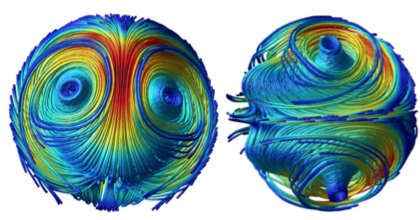
\includegraphics[height=0.3\textheight,width=0.6\hsize,angle=0,keepaspectratio]{./Image/Yamamoto_relaxation.png}
\caption{Relaxed magnetic field in Yamamoto's simulation.}\label{Mag2}
\end{figure}
 
 
%=============================================
\section{球の数値計算手法}

本研究は球体のシミュレーションを対象としているので、球ジオメトリの計算手法が必要不可欠である。この章では球の数値計算手法と本研究に用いられる座標格子「Yin--Yang--Zhong 格子」について説明する。
%=============================================
\subsection{時間積分法}
微分方程式を離散化して解く手法は数多く考案されている\cite{理工学のための数値計算法}。その中でも本研究では時間積分には4次のルンゲ・クッタ法を、空間微分には有限差分法を採用した。以下ではまず4次ルンゲ・クッタ法について説明する。

時間積分法の基本的なものに前進オイラー法がある。解きたい微分方程式が以下のように表せるとする。
\begin{equation} \label{function}
\frac{dq(t)}{dt} = f(q,t) 
\end{equation}
ここで時間を$t$、物理量を$q$とする。次にそれぞれを以下のように離散化する。
\begin{eqnarray}
t_j &=& \Delta t \times j      \\
q_j &=& q(t_j)      \\
f_j &=& f(q_j,t_j)     
\end{eqnarray}
$j$は0以上の整数とする。
前進オイラー法は(\ref{function})式を以下のように近似する方法である。
\begin{equation}
\frac{q_{j+1}-q_j}{\Delta t} = f_j 
\end{equation}
この式を変形させると
\begin{equation}
q_{j+1} = q_j + \Delta t \times  f_j 
\end{equation}
となる。前進オイラー法は微分方程式の最も簡単な近似解法である。「前進」というのは、前に進んだ$t_{j+1}$と$t_j$における$q$ の値を用いて近似を行なっているからである。一方4次ルンゲ・クッタ法は(\ref{function})式を以下のように近似する。
\begin{eqnarray}
q_{j+1} &=& q_j + \frac{\Delta t}{6}k_1 + \frac{\Delta t}{3}k_2 + \frac{\Delta t}{3}k_3 + \frac{\Delta t}{6}k_4 \\
k_1 &=& f(q_j,t_j)  \\
k_2 &=& f(q_j+\frac{\Delta t}{2}k_1,t_j+\frac{\Delta t}{2})  \\
k_3 &=& f(q_j+\frac{\Delta t}{2}k_2,t_j+\frac{\Delta t}{2})  \\
k_4 &=& f(q_j+\Delta tk_3,t_j+\Delta t)
\end{eqnarray}
前進オイラー法は単純だがその精度は1次$\mathcal{O} \left( \Delta t \right)$である。それに対し4次ルンゲ・クッタ法は4次精度$\mathcal{O} \left( \Delta t^4 \right)$なので十分に高い。上に述べた古典的4次ルンゲ・クッタ法の問題点は必要なメモリ量が多くなることだが、それらを削減する手法(ルンゲ・クッタ・ギル法など)が考案されている。本研究では古典的な4次ルンゲ・クッタ法を用いる。

\subsection{空間離散化手法}
ここでは本研究が空間微分の数値解法として用いた有限差分法を関数展開法と比べて説明する。有限差分法とは空間を有限個の格子(グリッド)で分割する方法を指し、関数展開法とは球面調和関数(4.2.2参照)などの展開用の関数を用いて離散的に式を展開する方法(スペクトル法とも呼ばれる)を指す。流体のシミュレーションは関数展開法を用いた研究が盛んである\cite{mininni2006magnetohydrodynamic}。なぜなら、関数展開法は球ジオメトリへの適応が容易であり、比較的少ない展開モード数でも高い精度の解が得られるからである。しかし、球面調和関数を用いた関数展開法には以下の2つの問題点がある:

\begin{enumerate}
  \renewcommand{\labelenumi}{(\arabic{enumi})}
  \item 展開モード数$L,M$での計算量は$\mathcal{O} \left( L^2 M^2 \right)$であるため、高い空間解像度を得るために展開モード数を増やすと計算量が非線形に増大してしまう。
  \item 数値計算の各ステップ毎に実空間とスペクトル空間の間で球面調和関数変換と逆変換を行う必要があるが、これらの処理にはプロセッサ間のグローバル通信が必要であり、並列計算に向かない。
\end{enumerate}

有限差分法は上記2つの問題点を解消することができる。
例えば、(1)に関して系の自由度を$L,M$とすると有限差分法の計算量は$\mathcal{O} \left( L M \right)$と表されるので、指数関数的に計算量が増えることはない。
また(2)に関して陽的な(未知の変数を既知の変数のみで直接求められる解法を陽解法という\cite{理工学のための数値計算法})時間積分法を採用する限り、グリッドベースの方法が並列計算に適していることはよく知られている。

よって有限差分法を用いてシミュレーションを行いたいのだが、有限差分法を球ジオメトリに適応させるには計算上の問題がある。次節では球座標格子の問題点について説明する。

\subsection{球座標格子の問題点}
従来、球ジオメトリの流体シミュレーションには球座標格子($r$,$\theta$,$\phi$)が広く使われてきた\cite{yoshimura1975model}\cite{chen2014global}。ここで$r$は原点からの距離(半径)、$\theta$は余緯度、$\phi$は経度である。球座標格子の低緯度表面付近は格子間隔がほぼ均一であり理想的なシミュレーション格子といえる。しかし、球座標格子には以下の2つの特異点がある[Fig.\ref{fig:grid}]:
\begin{description}
\item{(1)}極($\theta$ = 0,$\pi$)
\item{(2)}球の中心($r = 0$)
\end{description}
これらの特異点によって、シミュレーションにおいて2つの問題が生じる:
\begin{description}
\item{(1)}特異点でのゼロ除算の問題
\item{(2)}特異点に格子が集中していることによる計算コストの増加
\end{description}

(1)の問題については、シミュレーションにおいて座標特異点上に格子点を置く必要はなく、ずらして置くことが可能なので回避することができる\cite{kageyama1993simulation}。またロピタルの定理を利用し方程式を特異的でない形にして解くという方法もある\cite{kageyama1993simulation}。(1)の問題よりむしろ(2)の格子点が集中している問題のほうが深刻である。その理由について以下より説明する。

本研究ではMHD方程式を陽的な時間積分法である4次ルンゲ=クッタ法を用いて計算する。陽的な計算手法を用いて計算する場合、以下のCFL(Courant-Friedrichs-Lewy)条件を満たす必要がある。CFL条件とはシミュレーション内の情報が伝播する速さが物理的に計算される波の伝播速度を超えてはいけないという制約条件である(この制約を破るとシミュレーションで得られる数値に物理的な意味がなくなる)。例えば、音波モードのみが存在する1次元の系におけるCFL条件は以下の式で表される:
\begin{equation}
\Delta t < \alpha\frac{\Delta x}{C} 
\end{equation}
ここで$\Delta t$はシミュレーションの時間刻み幅、$\Delta x$はシミュレーションの格子間隔、$C$は音速、$\alpha$は定数である。
この式からシミュレーションの格子間隔が小さいほど、より短い時間刻み幅で数値解析を行う必要があることがわかる。
つまり、格子点が集中している特異点付近は時間刻み幅を小さくする必要があり、全ての格子点はその時間刻み幅に合わせなければならない。
よって、格子点の集中は計算コストの増大につながりシミュレーションの時間発展を妨げる障害となる。

この格子点の集中を避けるために考案されたのがYin--Yang--Zhong格子である\cite{hayashi2016yin}。

\begin{figure}[H]
\centering
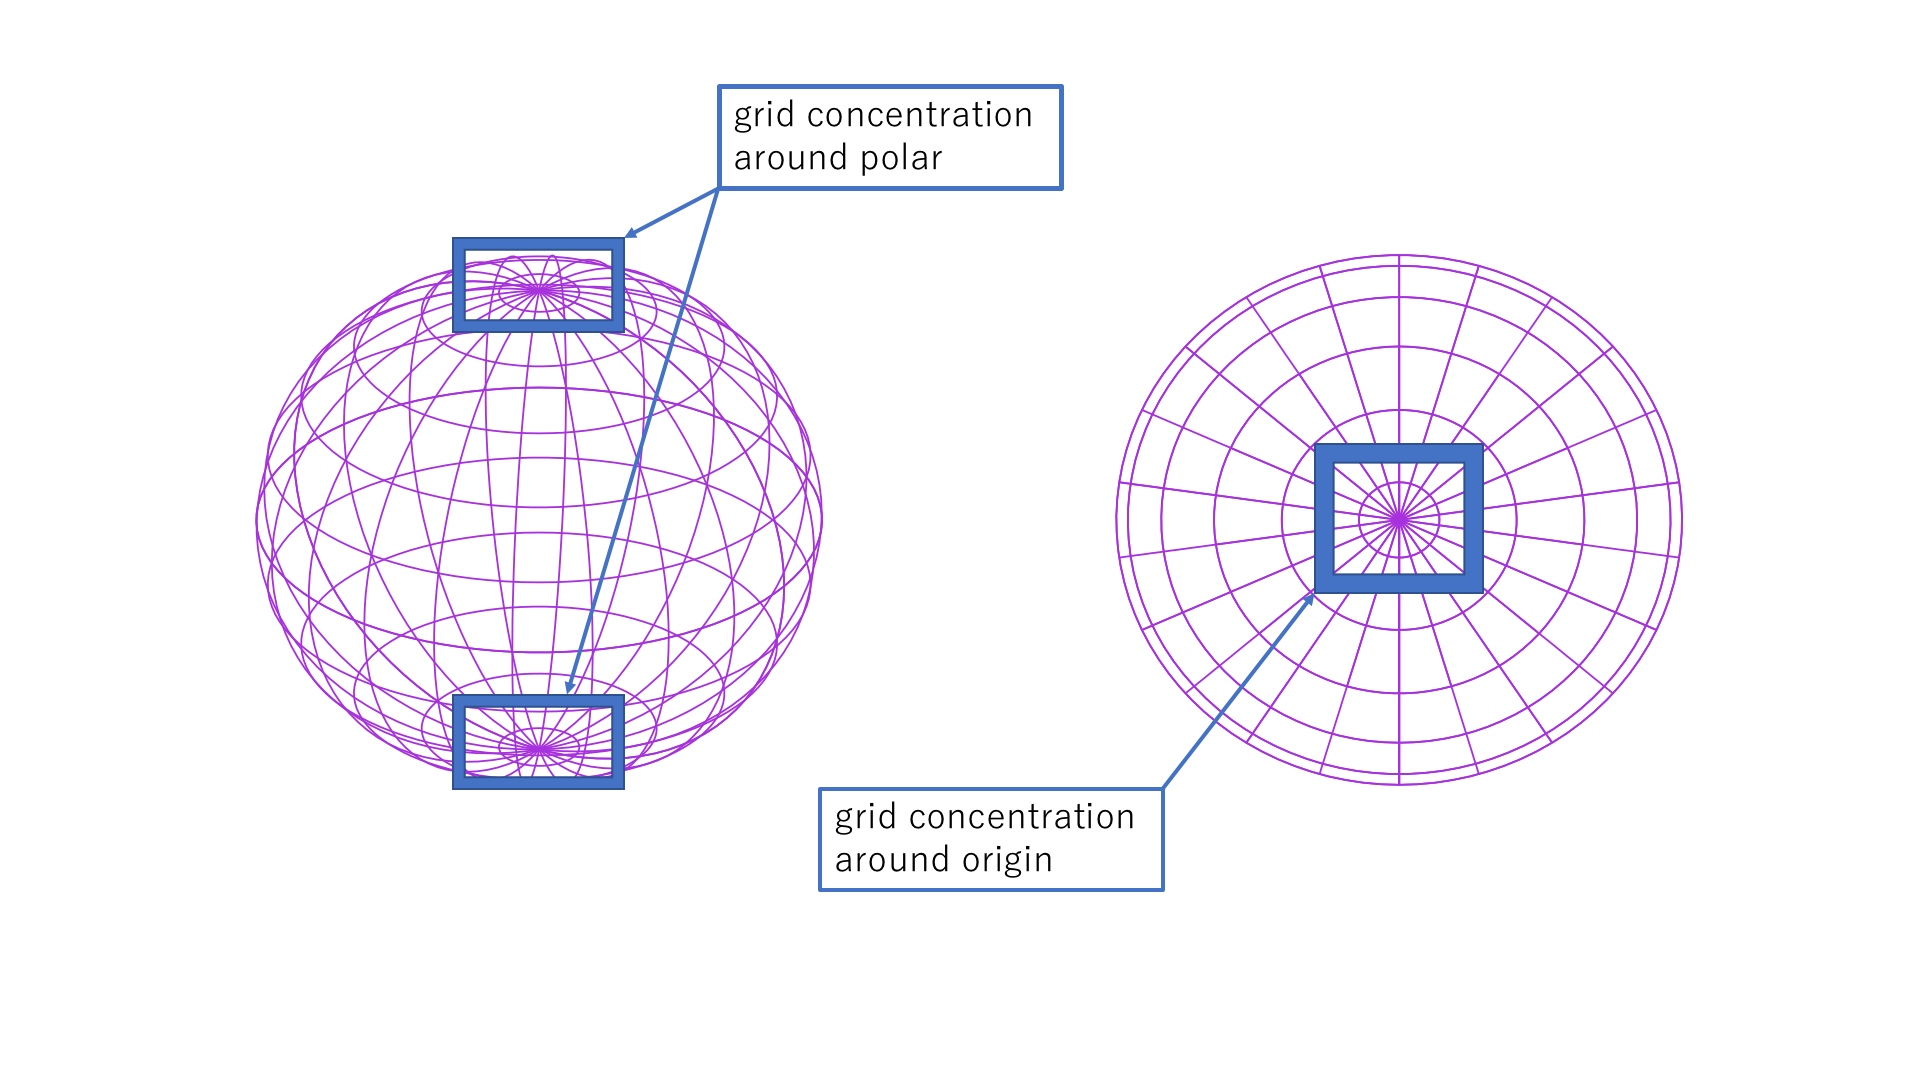
\includegraphics[height=0.5\textheight,width=1.0\hsize,angle=0,keepaspectratio]{./Image/grid.png}
\caption{Spherical polar coordinates. Grid points are concentrated around the poles and the origin.} \label{fig:grid}
\end{figure}



%=============================================
\subsection{Yin--Yang 格子の利点と Zhong 格子の導入}
ここでは、Yin--Yang--Zhong格子の前身となる「Yin--Yang 格子」 (Kageyama \& Sato \cite{kageyama2004yin})について説明する。Yin--Yang 格子とは、球座標格子の低緯度部分を切り取った格子を2つ組み合わせて球全体を覆う重合格子法の1つである。Yin--Yang 格子の構成要素は、球座標系の以下の余緯度$\theta$、経度$\phi$を切り取ったものである:
\begin{equation}
\frac{\pi}{4} \leq \theta \leq \frac{3\pi}{4}
\end{equation}
\begin{equation}
-\frac{3\pi}{4} \leq \phi \leq \frac{3\pi}{4}
\end{equation}

Yin 格子は、球座標系の式 (2),(3) の範囲の格子である。Yang 格子は Yin 格子と同形であり、軸を回転させたものである。Yin 格子とYang 格子の二つを組み合わせて球を覆うことによって外核を表現する。 Yin--Yang 格子は球座標格子の利点である低緯度部分を用いているので、極付近への格子の集中を避けることができる。シミュレーションでは、Yin 格子、Yang 格子ともに球座標格子系で計算を行い、それぞれの境界値を求める場合にはYang格子が本来、Yin格子の軸を回転させたものであることを考慮し、それぞれの格子で補間を行う。Yin-Yang 格子を用いた球殻シミュレーションは、地球科学と惑星科学\cite{peng2006conservative}、太陽物理学と宇宙物理\cite{shiota2010magnetohydrodynamic}、天体物理\cite{wongwathanarat2010axis}、画像処理\cite{hara2015gradient}など様々な研究に応用されている。
一方、Yin--Yang 格子を用いても球の原点付近での格子の集中は回避できない。そこで 新たに考案されたのが「Zhong 格子」である。Fig.\ref{fig:YYZthesis}に Yin--Yang--Zhong 格子の構造を示す。Zhong 格子は、Yin--Yang 格子で覆われた球中心の空洞部分に導入されるカーテシアン座標格子である。Yin--Yang 格子による球殻部分を Shell、Zhong 格子に よる球中心部分を Core と呼ぶ。Shell の内縁半径を$r_{c}$ とし、その内側に Core を配置する。 Yin--Yang--Zhong 格子を用いることで、ほぼ均一な格子間隔で全球シミュレーションを行うことが可能となる。
Yin--Yang--Zhong 格子を用いたシミュレーションでは、Yin 領域、Yang 領域、Zhong 領域 で別々の並列プロセスが割り当てられる。Core 領域である r = $r_{c}$ の球全体を囲む、一辺 が 2$r_{c}$ の立方体を l-cube と呼ぶ。ユーザーは、l-cube の x-y-z 方向の分割数を指定す る。分割したうちの 1 つの区画を s-cube と呼ぶ。Core 領域に少しでも重なっている部分 を持つ s-cube には並列プロセスを割り当て、Core 領域と重なった部分を持たない s-cube には並列プロセスを割り当てない。これにより、Shell 領域、Core 領域それぞれに効率よく並列プロセスを割り当てることができる。

\begin{figure}[H]
\centering
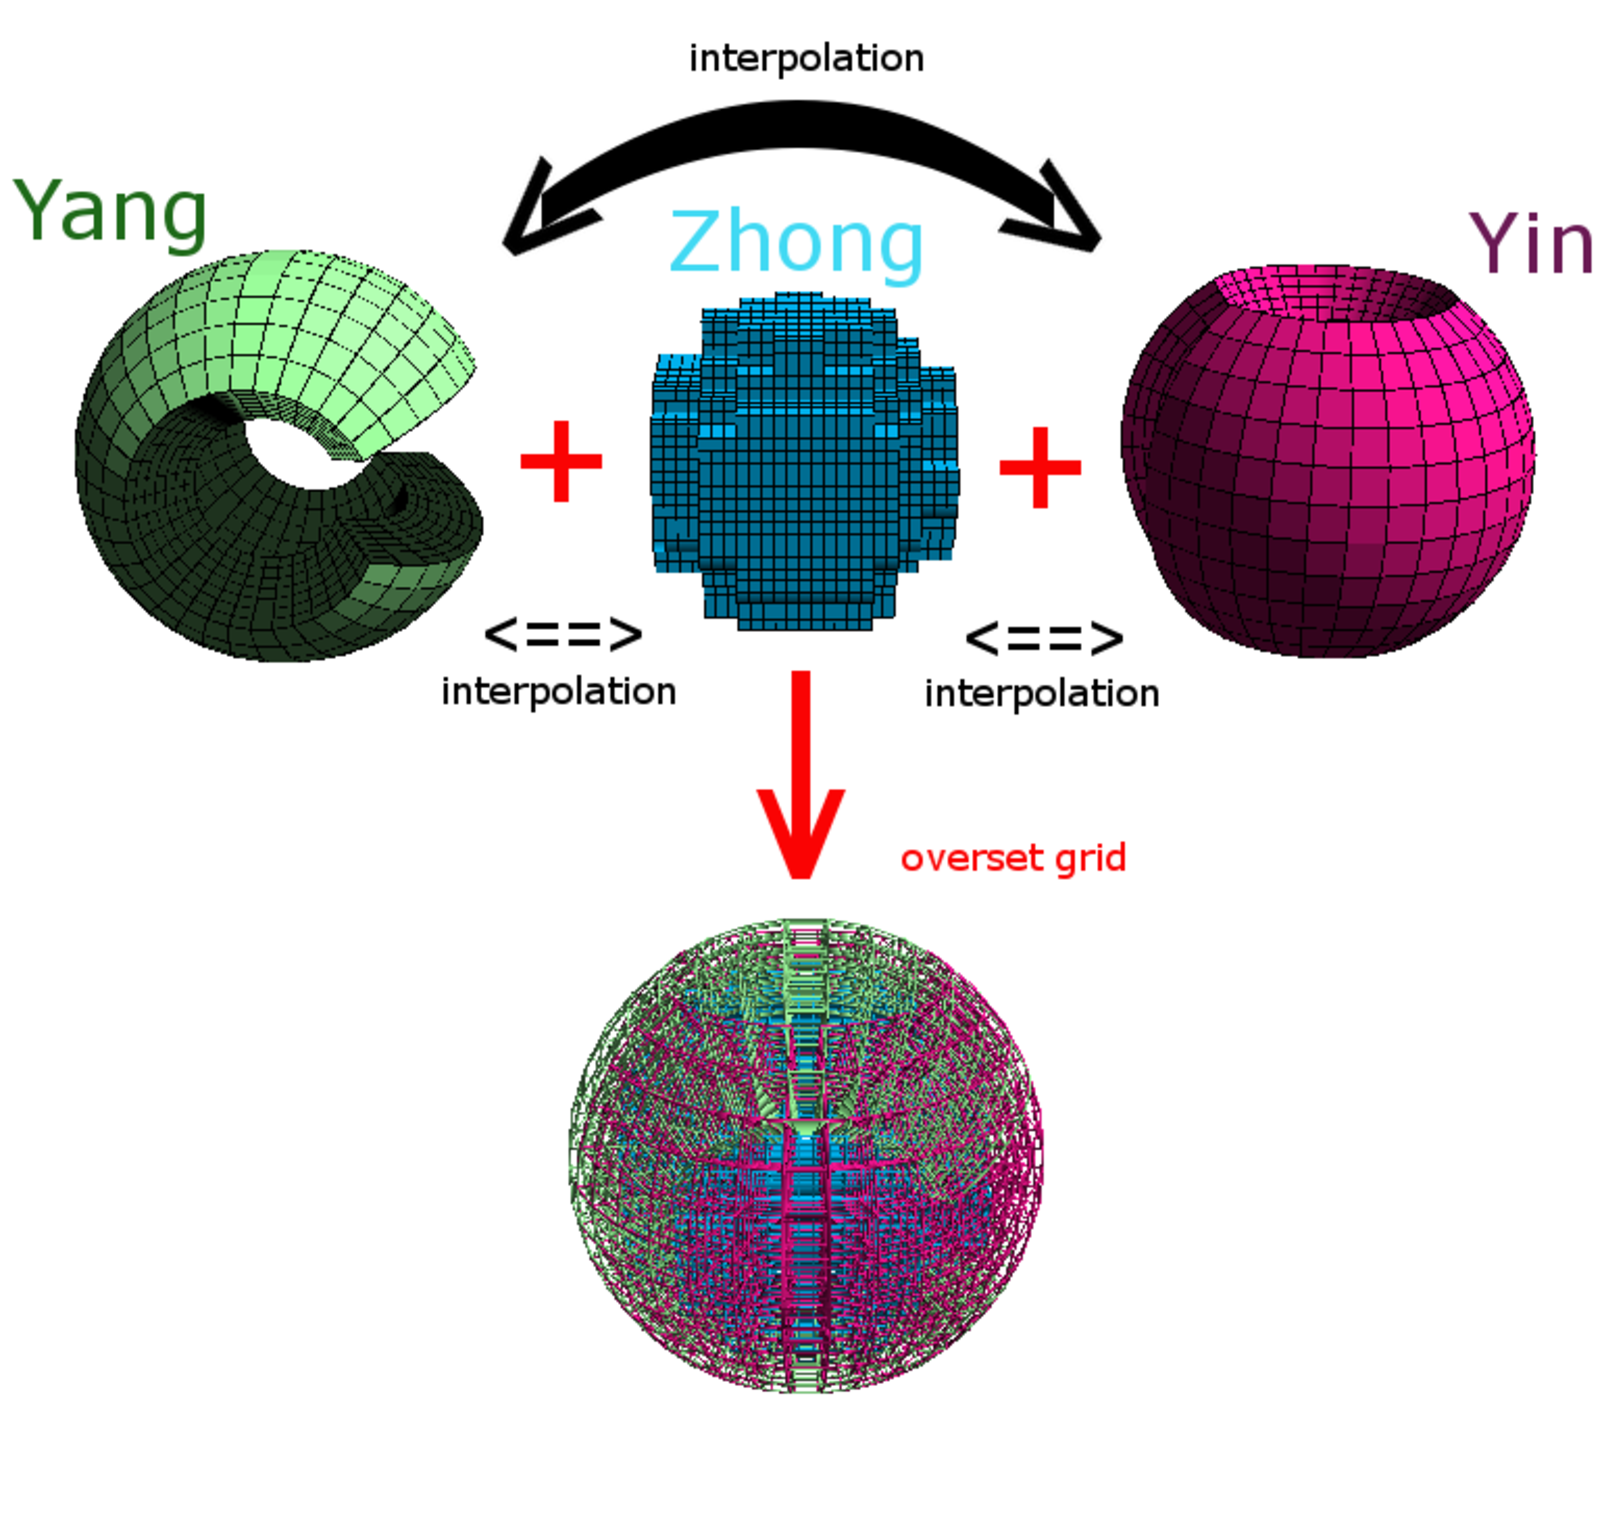
\includegraphics[height=0.75\textheight,width=1.0\hsize,angle=0,keepaspectratio]{./Image/YYZthesis.pdf}
\caption{Construction of Yin-Yang-Zhong grid.} \label{fig:YYZthesis}
\end{figure}

%=============================================
\subsection{Yin--Yang--Zhong 格子の座標変換}
 Yin格子とYang格子では、座標系が異なるが、元は同じ球座標系であるため、簡潔に座標変換を行うことができる。Yin領域における直交座標系($x^{e}$,$y^{e}$,$z^{e}$)とYang領域における直交座標系($x^{n}$,$y^{n}$,$z^{n}$)には、

\begin{equation}
\label{Yin-ortho}
(x^{e},y^{e},z^{e})=(-x^{n},z^{n},y^{n})
\end{equation}

\begin{equation}
\label{Yang-ortho}
(x^{n},y^{n},z^{n})=(-x^{e},z^{e},y^{e}) 
\end{equation}
という関係がある。これを行列で表現すると、
\begin{equation}
\label{Yin-Yang-matrix}
\begin{pmatrix}
x^{e} \\ y^{e} \\ z^{e}
\end{pmatrix} 
= 
M\begin{pmatrix}
x^{n} \\ y^{n} \\ z^{n}
\end{pmatrix}
\end{equation}
ここで、
\begin{equation}
\label{matrix}
M=
\begin{pmatrix}
-1 & 0 & 0 \\ 0 & 0 & 1 \\ 0 & 1 & 0
\end{pmatrix} 
\end{equation}
であり、この変換行列$M$は$M^{-1}=M$の関係を満たす。また式(\ref{Yin-ortho})-(\ref{matrix})より球座標形式での座標の関係は、
\begin{eqnarray}
r^{e}&=&r^{n}, \\
\sin\theta^{e}\cos\phi^{e}&=&-\sin\theta^{n}\cos\phi^{n}, \\
\sin\theta^{e}\sin\phi^{e}&=&\cos\phi^{n}, \\
\cos\phi^{e}&=&\sin\theta^{n}\sin\phi^{n}, 
\end{eqnarray}
で与えられることがわかる。ここでの添字の$n,e$はそれぞれYin座標とYang座標に対応する。

次にZhong格子について示す。Zhong格子は、一般的なカーテシアン座標系なので、Yin格子、Yang格子とZhong格子の間の座標変換はよく知られた極座標とカーテシアン座標の座標変換の式、
\begin{eqnarray}
x&=&r\sin\theta\cos\phi, \\
y&=&r\sin\theta\sin\phi, \\
z&=&r\cos\theta, \\
\end{eqnarray}
で与えられる。

 %=============================================
\subsection{Yin--Yang--Zhong格子のベクトル変換と補間}
Shellにおいて球殻がYin領域とYang領域の2つの領域に分割されているため、Yin格子とYang格子の境界部分で値の相互補完を行う必要がある。スカラー値の補間は単純だが、ベクトル値の補間はやや複雑である。これはYang格子はYin格子を回転させたものであり、ベクトルの方向がそれぞれの格子で異なるためである。

Fig.\ref{fig:sphericalNormalVectors}にYin格子とYang格子のベクトルの向きの関係を示す。図の緑色の格子がYin格子、青色の格子がYang格子を示している。図中の$\hat{\theta}^{n}$と$\hat{\phi}^{n}$は、それぞれYin格子の緯度方向、経度方向のベクトルであり、$\hat{\theta}^{e}$と$\hat{\phi}^{e}$はそれぞれYang格子の緯度方向、経度方向の単位ベクトルである。Yin格子上でのベクトル場を${(v^n_r,v^n_\theta,v^n_\phi)}^t$、Yang 格子上でのベクトル場を${(v^e_r,v^e_\theta,v^e_\phi)}^t$とする。ここで$t$は転置を意味する。Yin-Yang 格子間の回転角を$\psi(\theta,\phi)$とすると、Yin 座標から Yang 座標へのベクトル変換は、
\begin{equation}
\begin{pmatrix}
v^e_r \\ v^e_\theta \\ v^e_\phi  
\end{pmatrix} 
=
\begin{pmatrix}
1 & 0 & 0 \\ 0 & \cos\psi & -\sin\psi \\ 0 & \sin\psi & \cos\psi
\end{pmatrix} 
\begin{pmatrix}
v^n_r \\ v^n_\theta \\ v^n_\phi  
\end{pmatrix} 
\end{equation}
と表すことができる。$r$方向のベクトルは不変で、$\theta,\phi$方向のベクトルの回転変換を行っている。Fig.\ref{fig:sphericalNormalVectors}から、$\cos\psi$と$\sin\psi$は
\begin{eqnarray}
\cos\psi&=&\hat{\phi}^n \cdot \hat{\phi}^e, \\
\sin\psi&=&-\hat{\phi}^n \cdot \hat{\theta}^e ,
\end{eqnarray}
と表される。また、$\hat{\phi}^n,\hat{\phi}^e,\hat{\theta}^e$は、
\begin{eqnarray}
\hat{\phi}^n&=&-\sin\phi^n\hat{x}^n+\cos\phi^n\hat{y}^n, \\
&=&-\sin\phi^n\hat{x}^e+\cos\phi^n\hat{z}^e, \\
\hat{\phi}^e&=&-\sin\phi^e\hat{x}^e+\cos\phi^e\hat{y}^e, \\
\hat{\theta}^e&=&\cos\theta^e\cos\phi^e\hat{x}^e+\cos\theta^e\sin\phi^e\hat{y}^n-\sin\theta^e\hat{z}^e, 
\end{eqnarray}
と表すことができる。ここで、Yin格子、Yang格子でのカーテシアン座標系の各単位ベクトルをそれぞれ$\hat{x}^n,\hat{y}^n,\hat{z}^n,\hat{x}^e,\hat{y}^e,\hat{z}^e$とした。よって、$\cos\psi$と$\sin\psi$は、式(50)-(55)より、
\begin{eqnarray}
\cos\psi&=&-\sin\phi^e\sin\phi^n, \\
\sin\psi&=&\frac{\cos\phi^n}{\sin\theta^e} 
\end{eqnarray}
とかける。式 (22),(23) を用いると、Yin--Yang 格子におけるベクトル変換式は、変換行列
 を$P$とし、
\begin{equation}
\begin{pmatrix}
v^e_r \\ v^e_\theta \\ v^e_\phi  
\end{pmatrix} 
=
P
\begin{pmatrix}
v^n_r \\ v^n_\theta \\ v^n_\phi  
\end{pmatrix} ,
\end{equation}
\begin{equation}
P=
\begin{pmatrix}
1 & 0 & 0 \\ 0 & -\sin\phi^e\sin\phi^n & -\cos\phi^n/\sin\theta^e \\ 0 & \cos\phi^n/\sin\theta^e & -\sin\phi^e\sin\phi^n
\end{pmatrix} ,
\end{equation}
と書くことができる。これは、Yin座標系からYang座標系への変換行列である。また、Yang座標系からYin座標系への変換行列は$P$の逆行列$P^{-1}$で表すことができ、$P^{-1}$は$P$の添字を入れ替えることで表現できる。
\begin{equation}
P^{-1}=
\begin{pmatrix}
1 & 0 & 0 \\ 0 & -\sin\phi^n\sin\phi^e & -\cos\phi^e/\sin\theta^n \\ 0 & \cos\phi^e/\sin\theta^n & -\sin\phi^n\sin\phi^e
\end{pmatrix} ,
\end{equation}
Zhong格子上でのベクトル場を$v_x,v_y,v_z$とすると、Zhong座標系からYin座標系へのベクトル変換は
\begin{equation}
\begin{pmatrix}
v^n_r \\ v^n_\theta \\ v^n_\phi  
\end{pmatrix} 
=
\begin{pmatrix}
\sin\theta\cos\phi & \sin\theta\sin\phi & \cos\theta \\ \cos\theta\cos\phi & \cos\theta\sin\phi & -\sin\theta \\ -\sin\phi & \cos\phi & 0
\end{pmatrix} 
\begin{pmatrix}
v_x \\ v_y \\ v_z  
\end{pmatrix} ,
\end{equation}
またZhong座標系からYang座標系へのベクトル変換は
\begin{equation}
\begin{pmatrix}
v^e_r \\ v^e_\theta \\ v^e_\phi  
\end{pmatrix} 
=
\begin{pmatrix}
-\sin\theta\cos\phi & -\sin\theta\sin\phi & -\cos\theta \\ -\sin\phi & \cos\phi & 0 \\ \cos\theta\cos\phi & \cos\theta\sin\phi & -\sin\theta
\end{pmatrix} 
\begin{pmatrix}
v_x \\ v_y \\ v_z  
\end{pmatrix} ,
\end{equation}
と表すことができる。Shell と Core の間の補間にはトリリニア補間を用いる。つまり、Shell の境界値を Core から補間 する場合は、半径 $r = r_c$ での Shell の座標値を Core の座標系に変換、補間点を囲む8個の格子点を探索し8点から線形補間を行う。逆に、Core の値を Shell から補間する場合 には、Shell の格子での、
\begin{equation}
r_c \leq r \leq r_c + 2\Delta r
\end{equation}
の範囲内で Core 領域に含まれる格子を探索する。そして、その座標値を Core から Shellに変換し、線形補間に利用する8つの格子点を探索し補間する。

\begin{figure}[H]
\centering
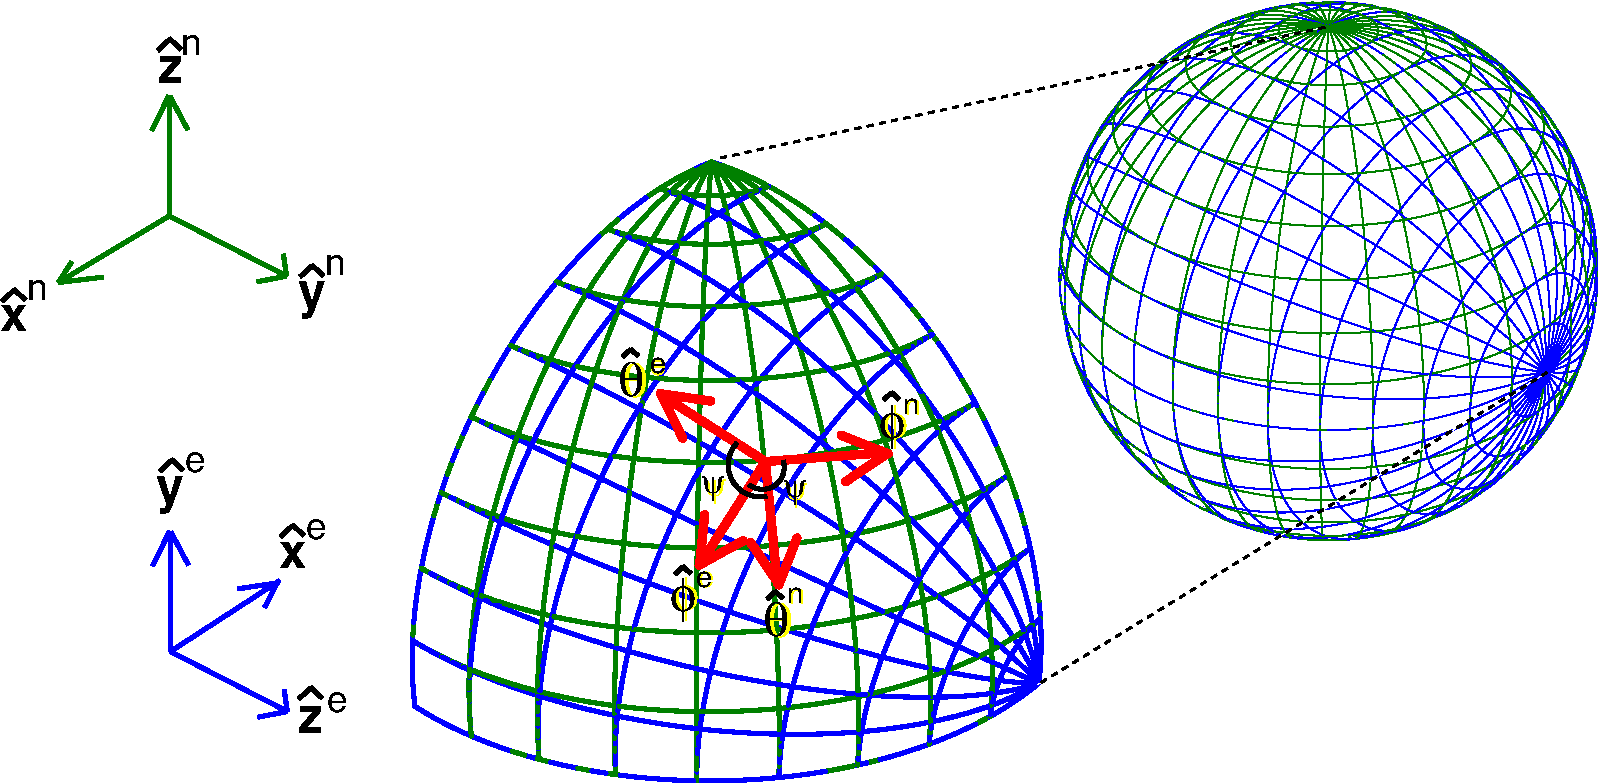
\includegraphics[height=0.75\textheight,width=1.0\hsize,angle=0,keepaspectratio]{./Image/sphericalNormalVectors.pdf}
\caption{Vector components of Yin and Yang.} \label{fig:sphericalNormalVectors}
\end{figure}

%=============================================
\section{Fortranプリプロセッサの開発}
球内部のMHD緩和現象を解明するために当研究室では数年前からYin--Yang--Zhong格子に基づくシミュレーションプログラムを開発し、改訂を続けてきた。このシミュレーションコードは現在ではかなり規模の大きなものである。シミュレーションモデルの変更に合わせて現在でもシミュレーションコードは絶え間なく改訂を続けているが、コードの複雑さが増大したためにバグの混入のない安全な改訂を継続的に進めることが困難になってきた。このシミュレーションコードはFortranで書かれている。そこで、より便利で簡潔なコーディングを目指すべくFortranのプリプロセッサを開発した。
%=============================================
\subsection{現代的Fortranの問題点}
Fortranとは1950年代に誕生した世界初の高級プログラミング言語の一つであり、その特徴はHPC (High Performance Computing:高性能計算)に特化していることである。FortranがHPCとして優れている点は以下の通りである:


\begin{itemize}
\item 多次元配列の扱いが得意であること。
\item 組み込み関数が豊富であること。
\item 数式の取り扱いが得意であること。
\item モジュールと内部副プログラムによる階層的名前空間が容易であること。
\item 数学ライブラリを含めて科学技術関係のコードが豊富であること。
\end{itemize}

Fortranは現在でもバージョンアップし続け、特にFortran 2003では大きな仕様変更がされた。Fortran 2003以降のバージョンを現代的Fortran (Modern Fortran)と呼ぶことが多い。
この現代的Fortranには様々な便利な機能を備えているものの、シミュレーションにおいては使いづらいところがある。例えば、CやJavaに標準的に用意されている複数行をまとめてコメントアウトする機能(ブロックコメントアウト)は現代的Fortranに備わっていないので、一行一行の行頭に「!」(exclamation mark)をつける必要がある(Fig.\ref{block-comment1})。これはトライ&エラーを繰り返す数値シミュレーションを行うものにとって大きな手間となり負担となる。このようなストレスがかかるコーディングを避けるために、新しいFortranの方言eFortranとそれを標準Fortranに文字列変換するプリプロセッサefppを開発した。

\begin{figure}[H]
\centering
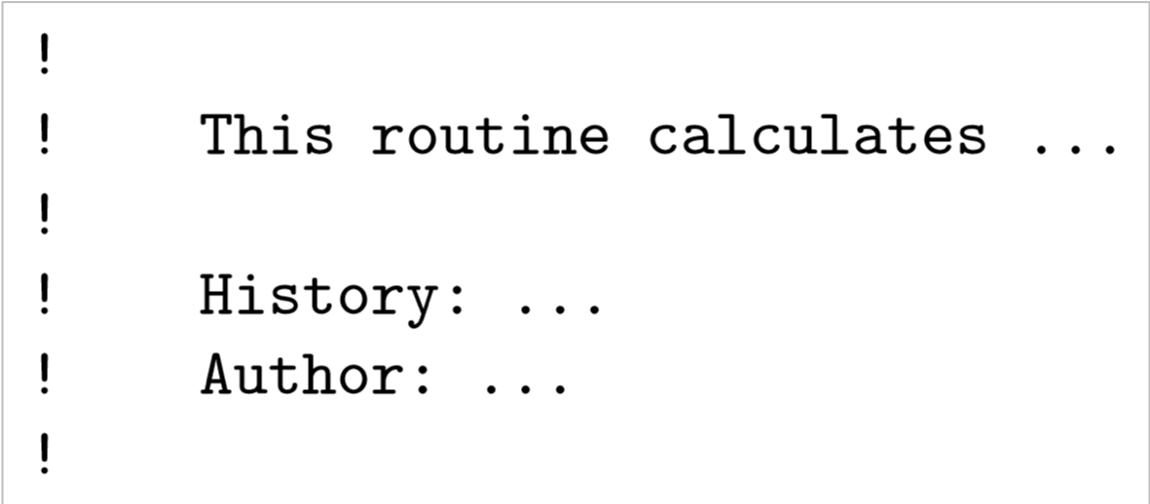
\includegraphics[height=0.5\textheight,width=1.0\hsize,angle=0,keepaspectratio]{./Image/block_comment1.png}
\caption{There is no block commets in standard Fortran.} \label{block-comment1}
\end{figure}


\subsection{eFortranとefpp}
プリプロセッサとはプログラムをコンパイルする前にそのプログラムになんらかの処理をするプログラムのことである。Fortranのプリプロセッサは以前より研究されてきた\cite{kernighan1975ratfor}\cite{tsuji1988structured}が、それらのプリプロセッサは主に構造的でなかった(goto文を使用していた)昔のFortranを構造的にするために使われていた。本研究で開発したプリプロセッサefppは通常コンパイルできない特殊な文法のプログラムを文字列置換によってコンパイル可能なプログラムに書き換える。我々はこの特殊な文法のプログラミング言語(方言)をeFortranと名付けた。つまり、eFortranで書かれたプログラムをefppによってコンパイル可能なプログラムに書き換えるという仕組みである(Fig.\ref{conversion})。efppはPythonで書いた。その理由は文字列変換に用いる正規表現が得意であることなどである。

\begin{figure}[H]
\centering
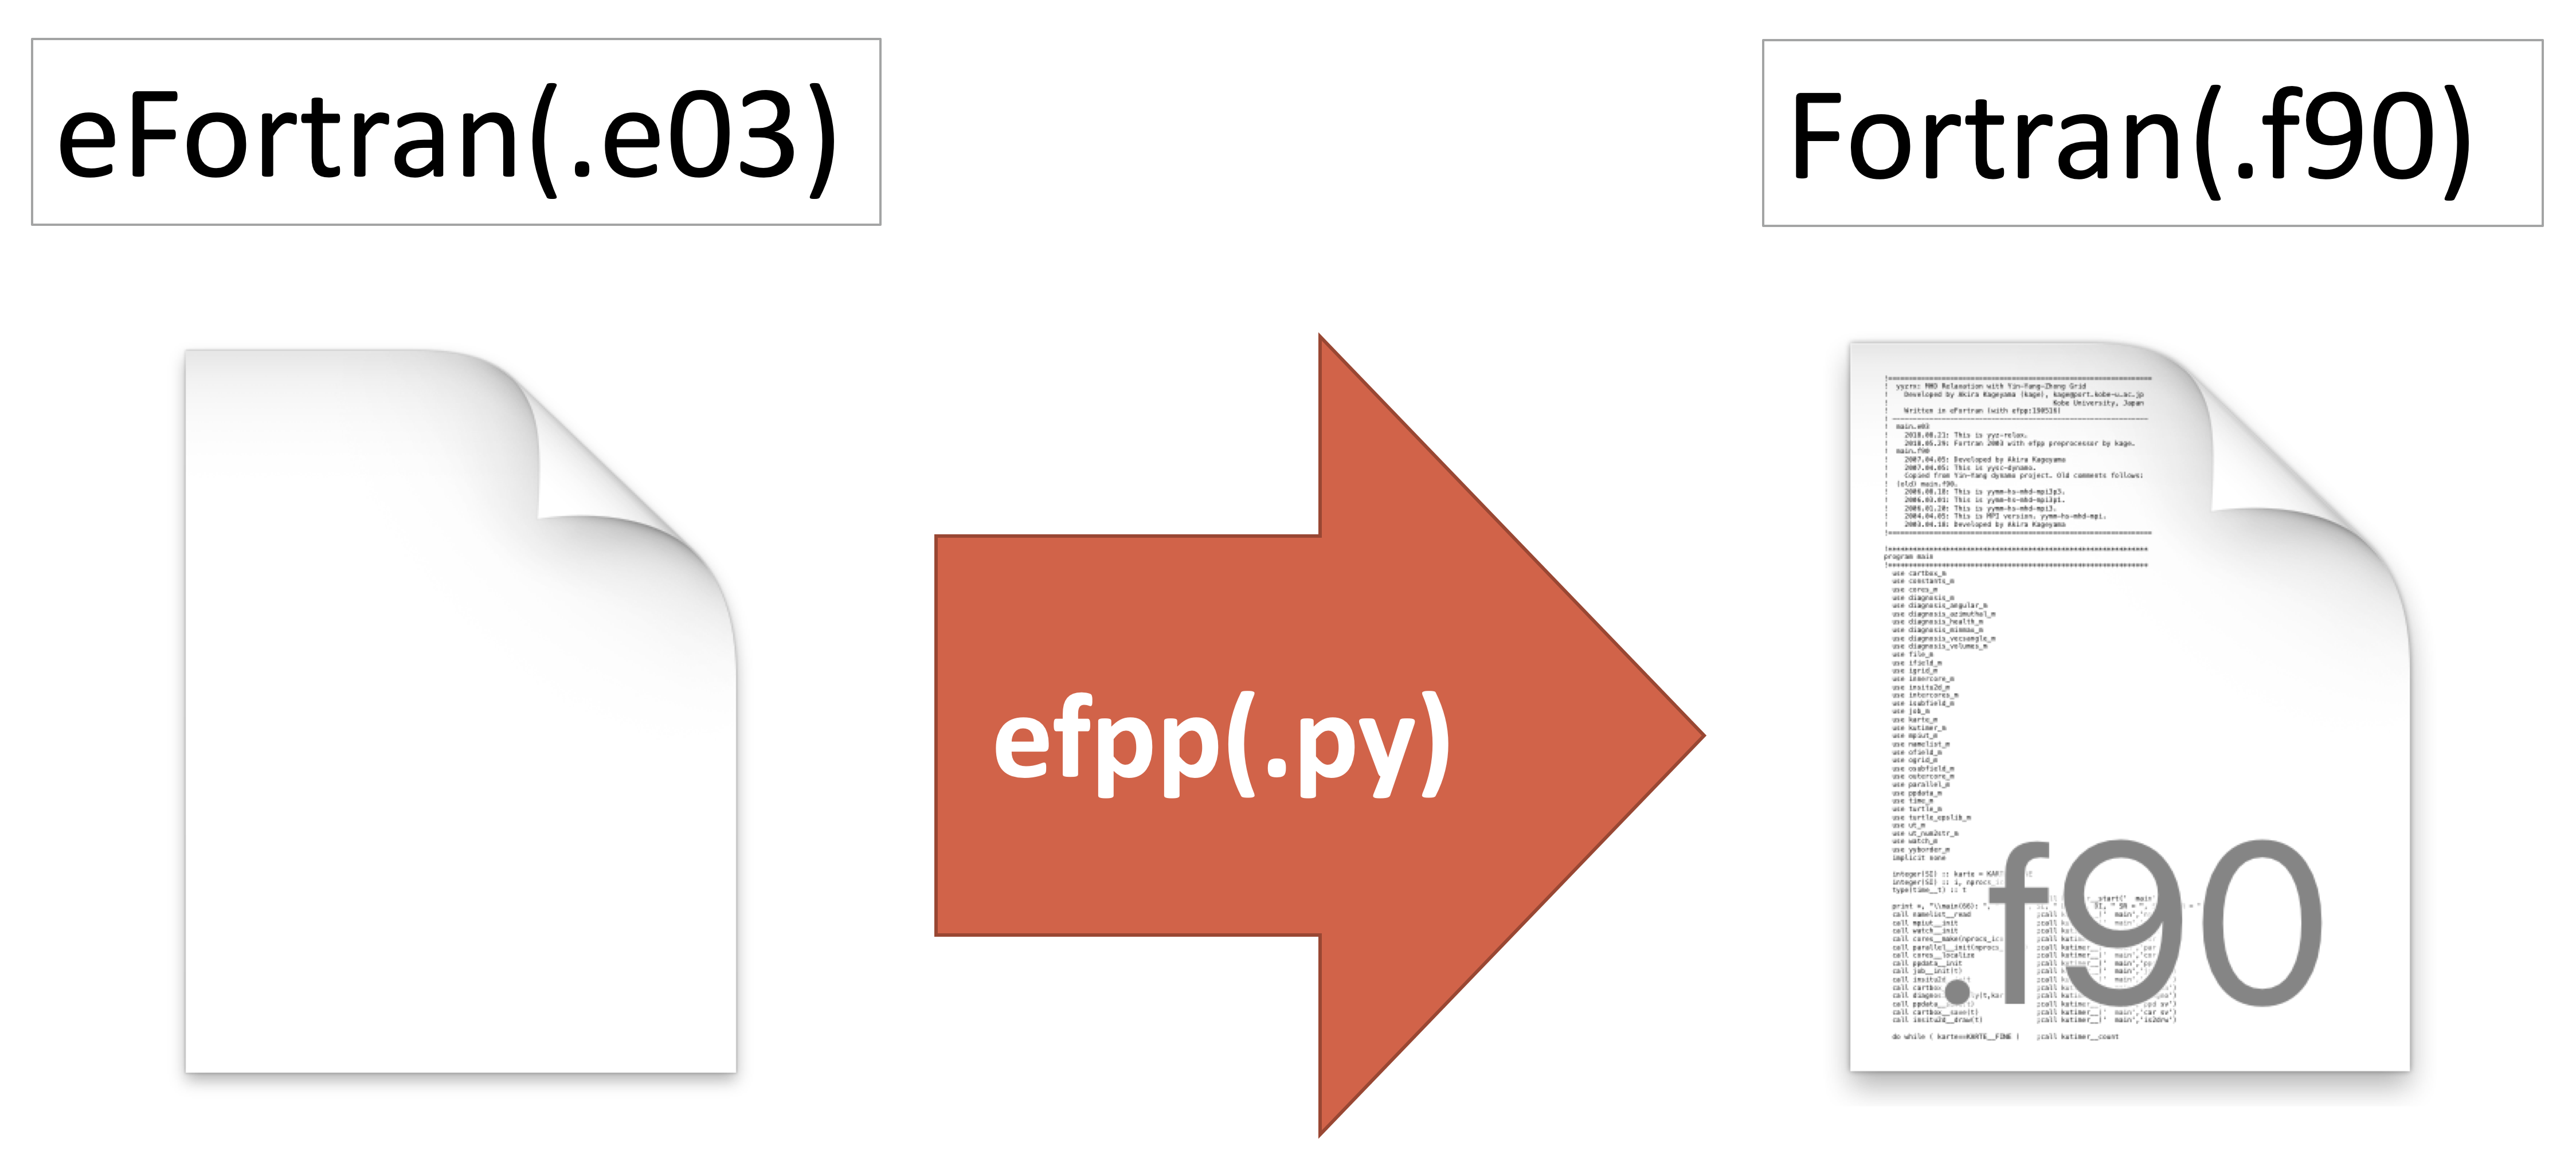
\includegraphics[height=0.5\textheight,width=1.0\hsize,angle=0,keepaspectratio]{./Image/conversion.png}
\caption{Conversion from eFortran to Fortran by preprocesser.} \label{conversion}
\end{figure}


efppの機能として
\begin{itemize}
\item シミュレーションでよく使う構文を簡潔に書くことができる。(繰り返し、初期化、変数定義など)
\item efppは実質文字列を変換しているだけなので、ユーザーが新しい文法を追加したり、必要ない文法を無視したりすることができる。
\item 文字列変換によって行番号を変えないようにしている、これはデバグの際に混乱することを避けるためである。
などが挙げられる。
\end{itemize}

\subsection{具体例}
ここでは3つの具体例を通して、eFortranの詳細を説明する。
\begin{description}
\item{(1)}ブロックコメント
\item{(2)}変数定義の簡略化
\item{(3)}マクロ定義
\end{description}

\subsubsection{ブロックコメント}
先ほど述べた通り、標準のFortranにはブロックコメント機能がないので複数行のコメントアウトには不便が生じていた。
そこでeFortranでは簡単に複数行のコメントアウトができるような新しい文法を追加した。
具体的にはコメントアウトしたい行を3つ以上の「=」(equal)の行で挟むことで実現する(Fig.\ref{block-comment2})。
この機能は入れ子にすることも可能で、eFortranコード内で同じ数の「=」の行のペアがあればそのペアに挟まれている行が自動的にコメントアウト文に変換される(Fig.\ref{block-comment3})。

\begin{figure}[H]
\centering
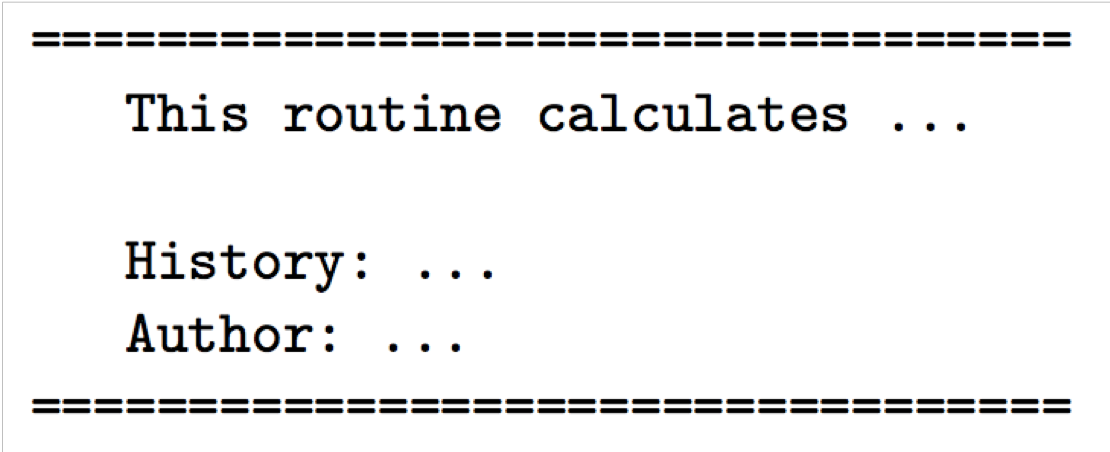
\includegraphics[height=0.5\textheight,width=1.0\hsize,angle=0,keepaspectratio]{./Image/block_comment2.png}
\caption{Syntax of block comment. Sandwiched by a pair of "=" sequence in eFortran.} \label{block-comment2}
\end{figure}
\begin{figure}[H]
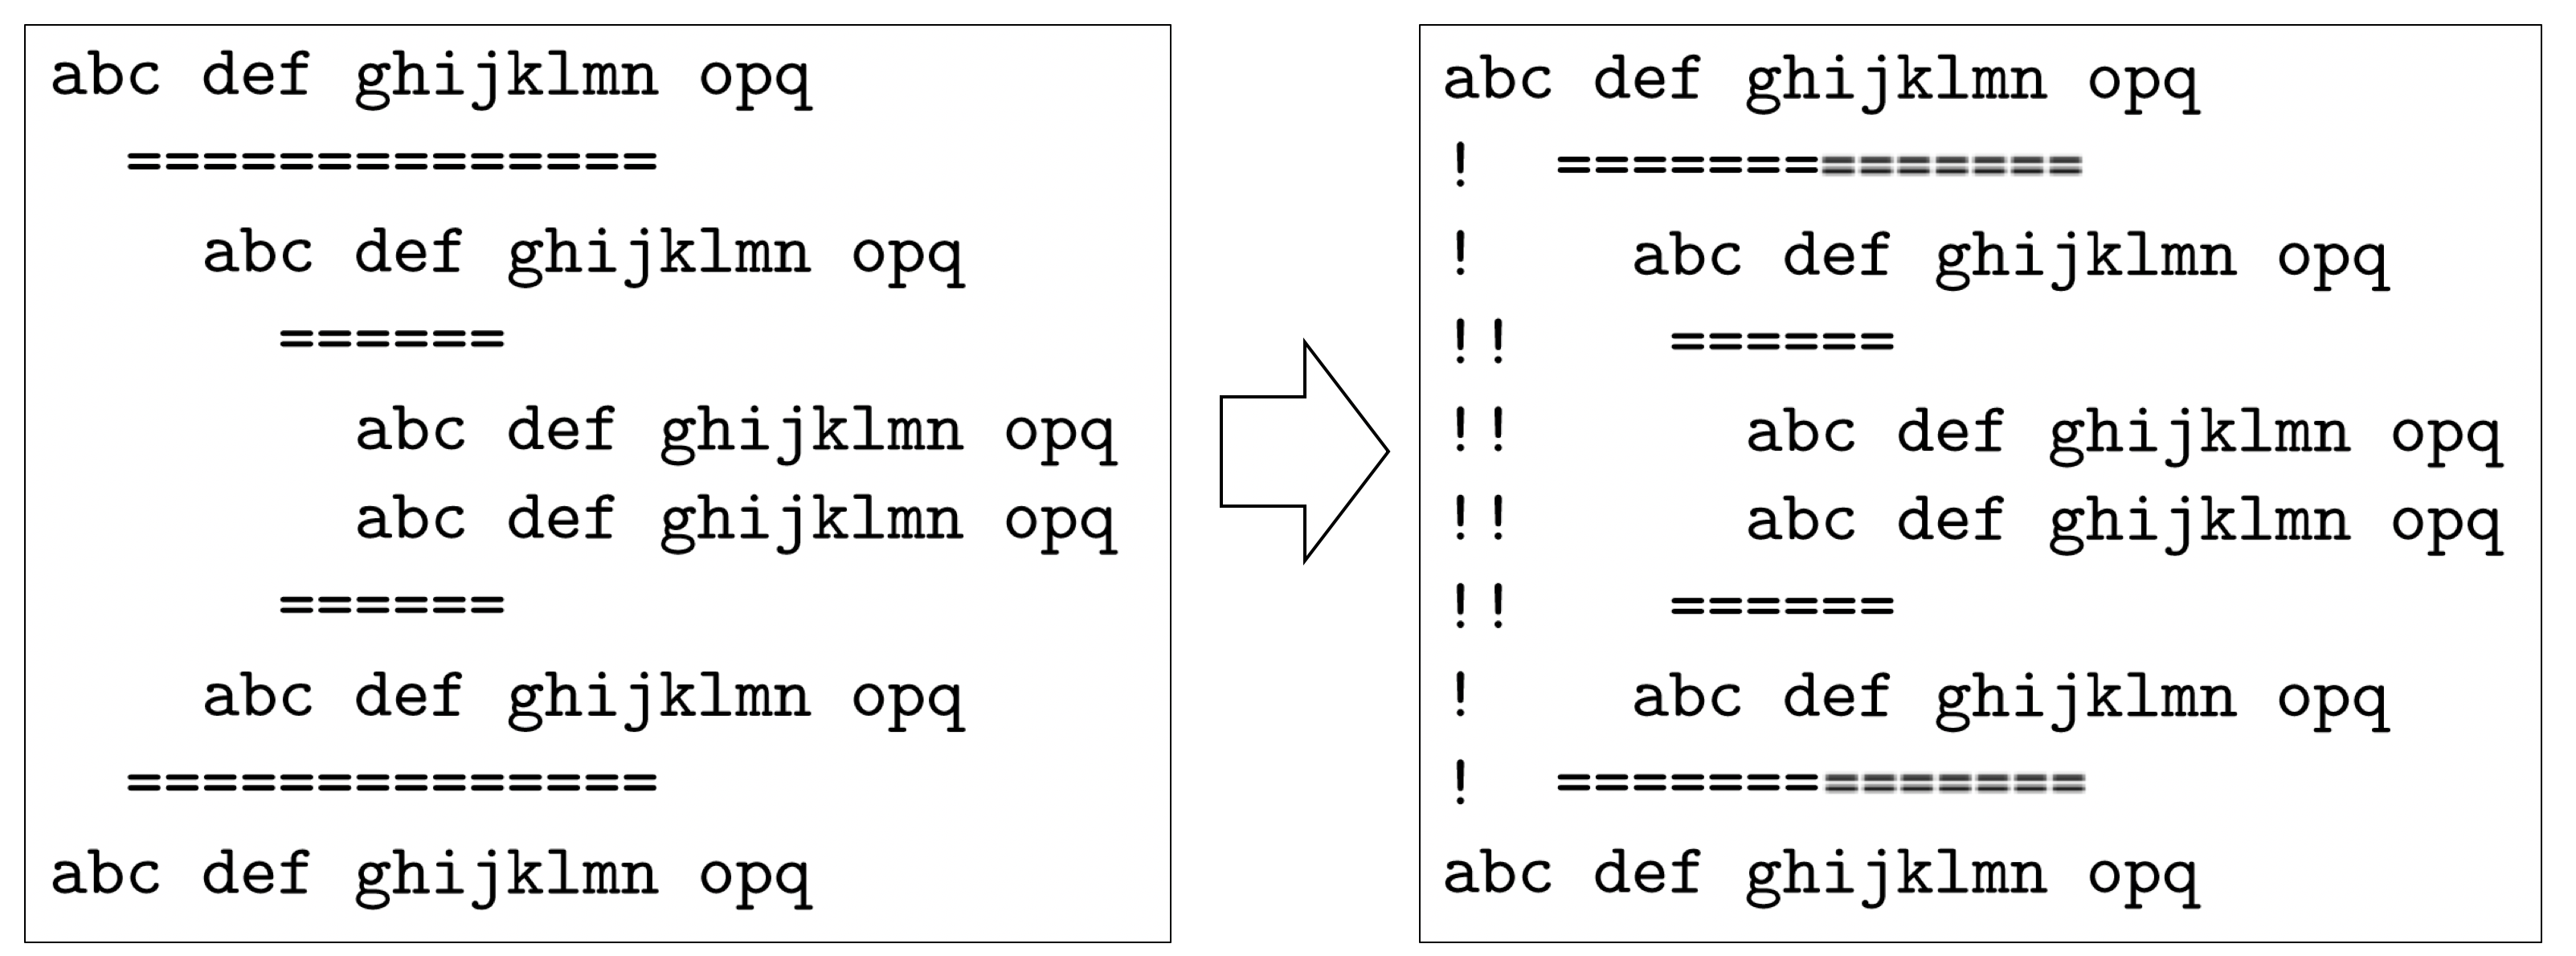
\includegraphics[height=0.5\textheight,width=1.0\hsize,angle=0,keepaspectratio]{./Image/block_comment3.png}
\caption{A block of comment can contain another block of comment inside it.} \label{block-comment3}
\end{figure}

\subsubsection{変数定義の簡略化}
Fortranの変数定義はCやJavaと違って、非常に冗長である。
例えば、整数型の変数$i$を定義するときはCでは
\begin{lstlisting}[language=c++]
int i;
\end{lstlisting}

\noindent
と書くのに対しFortranでは

\begin{lstlisting}[language=fortran]
integer :: i
\end{lstlisting}

\noindent
と書く必要がある。またFortranでは変数に様々なオプションをつける場合があり、例えば読み取り専用のオプショナル(省略可能な)引数である倍精度実数$p$は以下のように記述する。

\begin{lstlisting}[language=fortran]
real(DR), intent(in), optional :: p
\end{lstlisting}

\noindent
シミュレーションにおいて、このような変数定義は頻繁に行うためコーディングが面倒なだけでなくタイプミスによるエラーが起こりやすい。eFortranでは簡潔な変数定義を実現している。(Fig.\ref{declarations})

\begin{figure}[H]
\centering
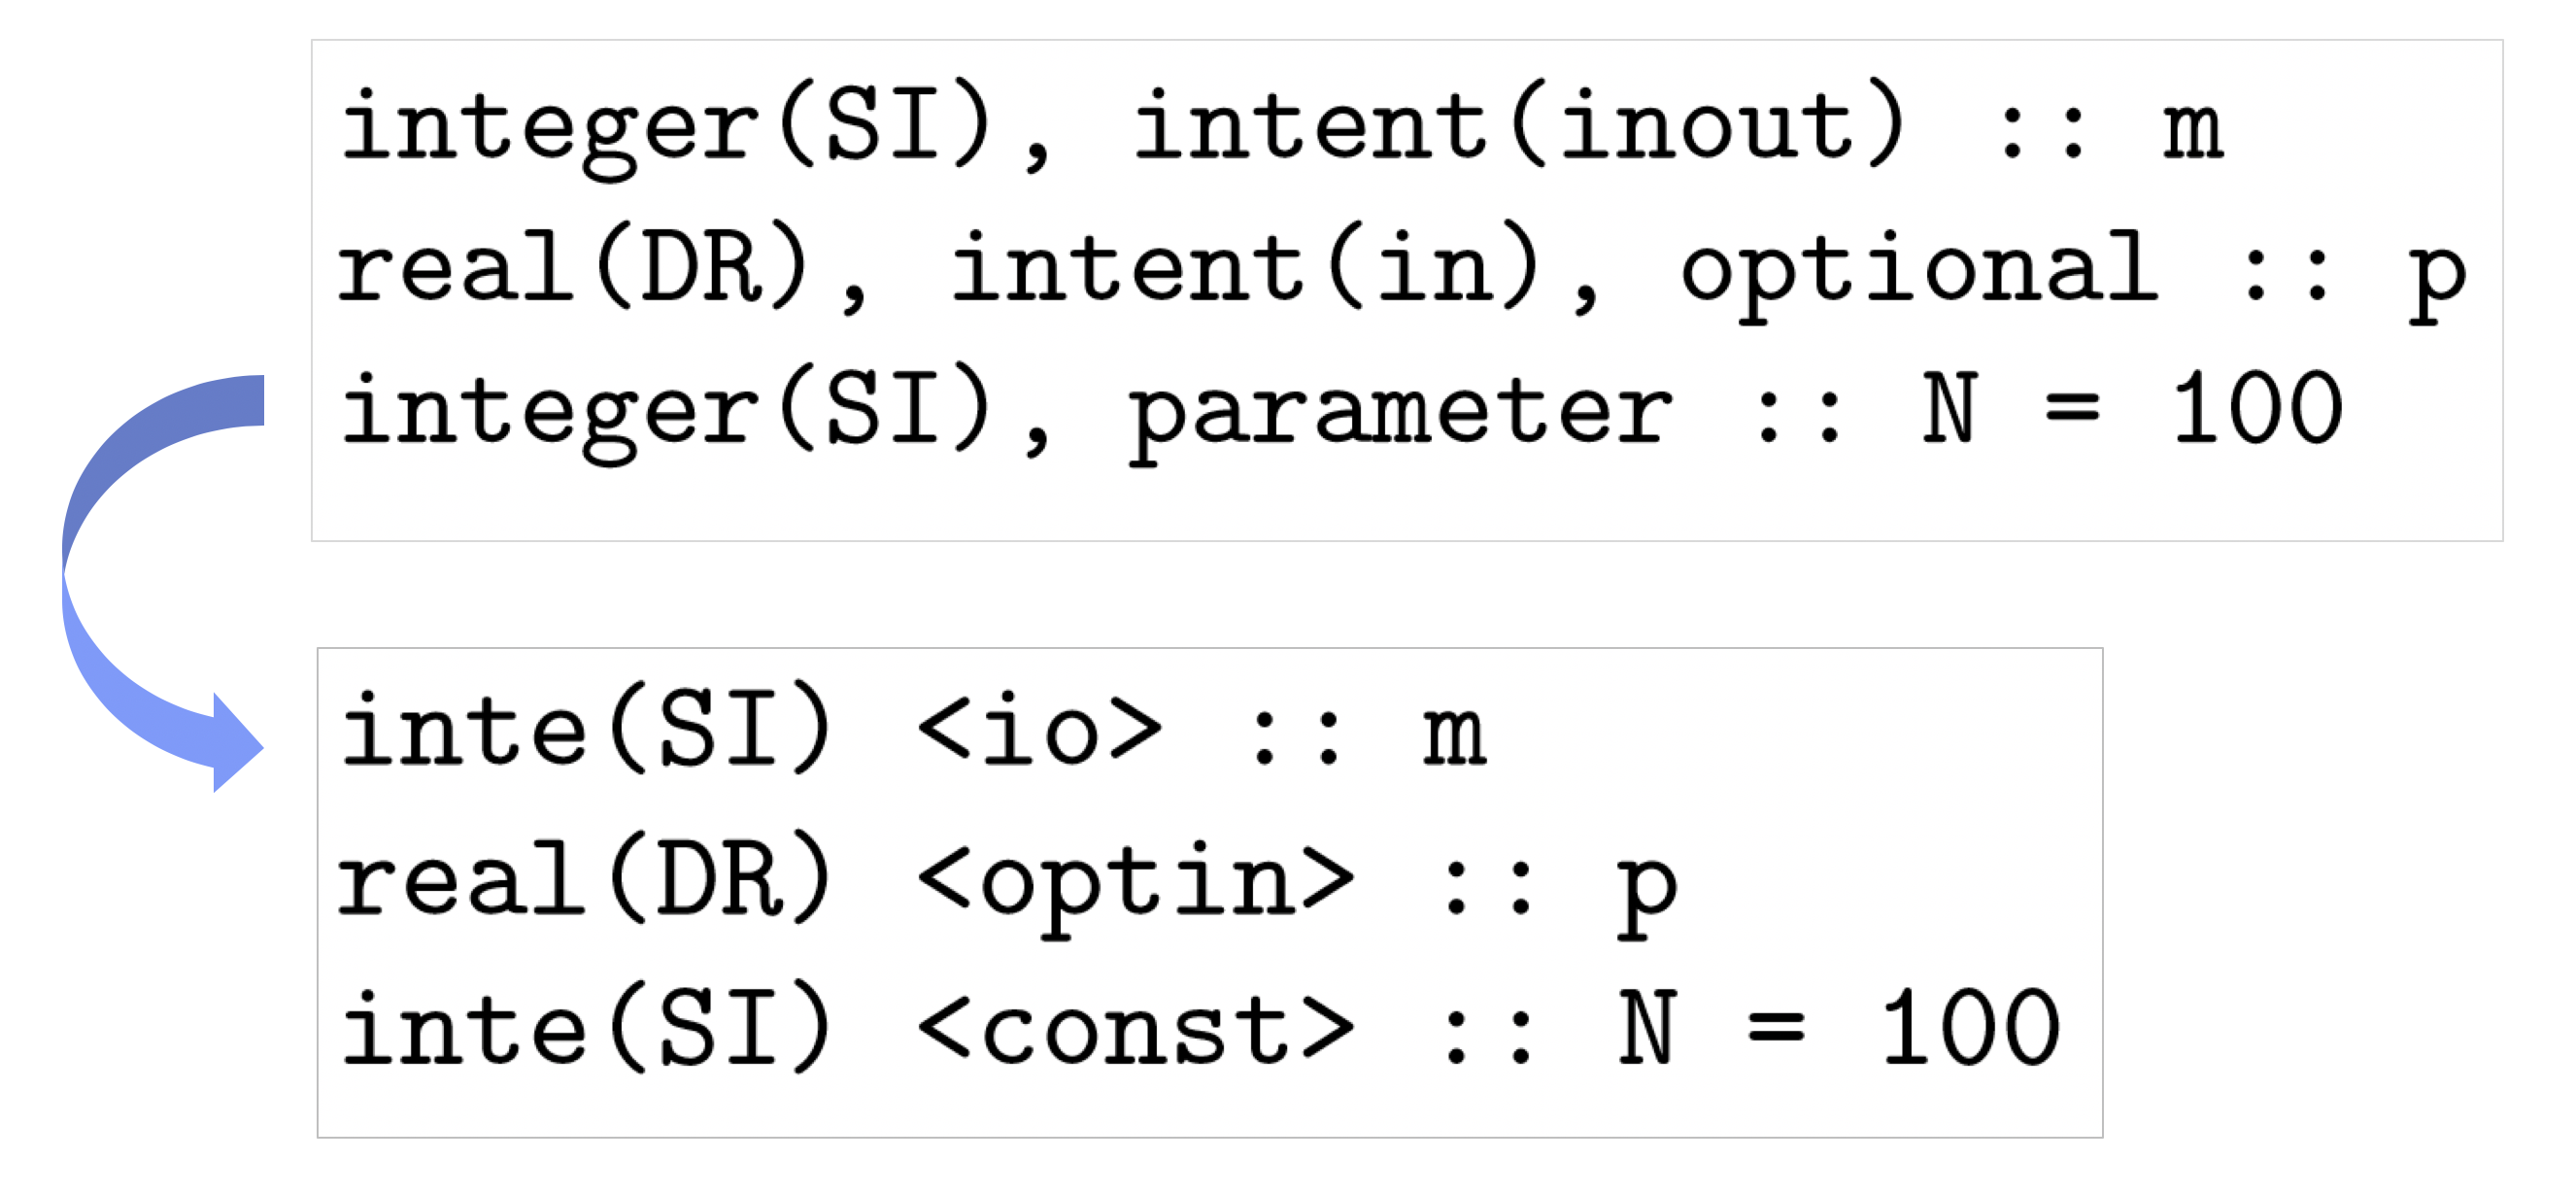
\includegraphics[height=0.5\textheight,width=1.0\hsize,angle=0,keepaspectratio]{./Image/declarations.png}
\caption{In standard Fortran, variable are some times too long declarations (top). On the other hand in eFortran, they can be short (bottom).} \label{declarations}
\end{figure}

\subsubsection{マクロ定義}
eFortranには特定の文字列をモジュール名や関数名などに自動的に変換する機能がある。
例えば、eFortranコードに「\_\_MODULE\_\_」と入力すれば、その文字列は「\_\_MODULE\_\_」と書かれたモジュールの名前に変換される。(Fig.\ref{macros})
この機能は主にデバグの際に用いられる。
さらに、このような文字列変換のルールはeFortranのユーザーが新しく作ることができる。
その方法はefpp\_alias.listというファイルに以下の文を追加すれば良い。
\begin{lstlisting}
"string_before" => "string_after"
\end{lstlisting}
これにより、eFortranコードで「string\_before」と書かれた箇所は標準Fortranコードで「string\_after」に変換される。

\begin{figure}[H]
\centering
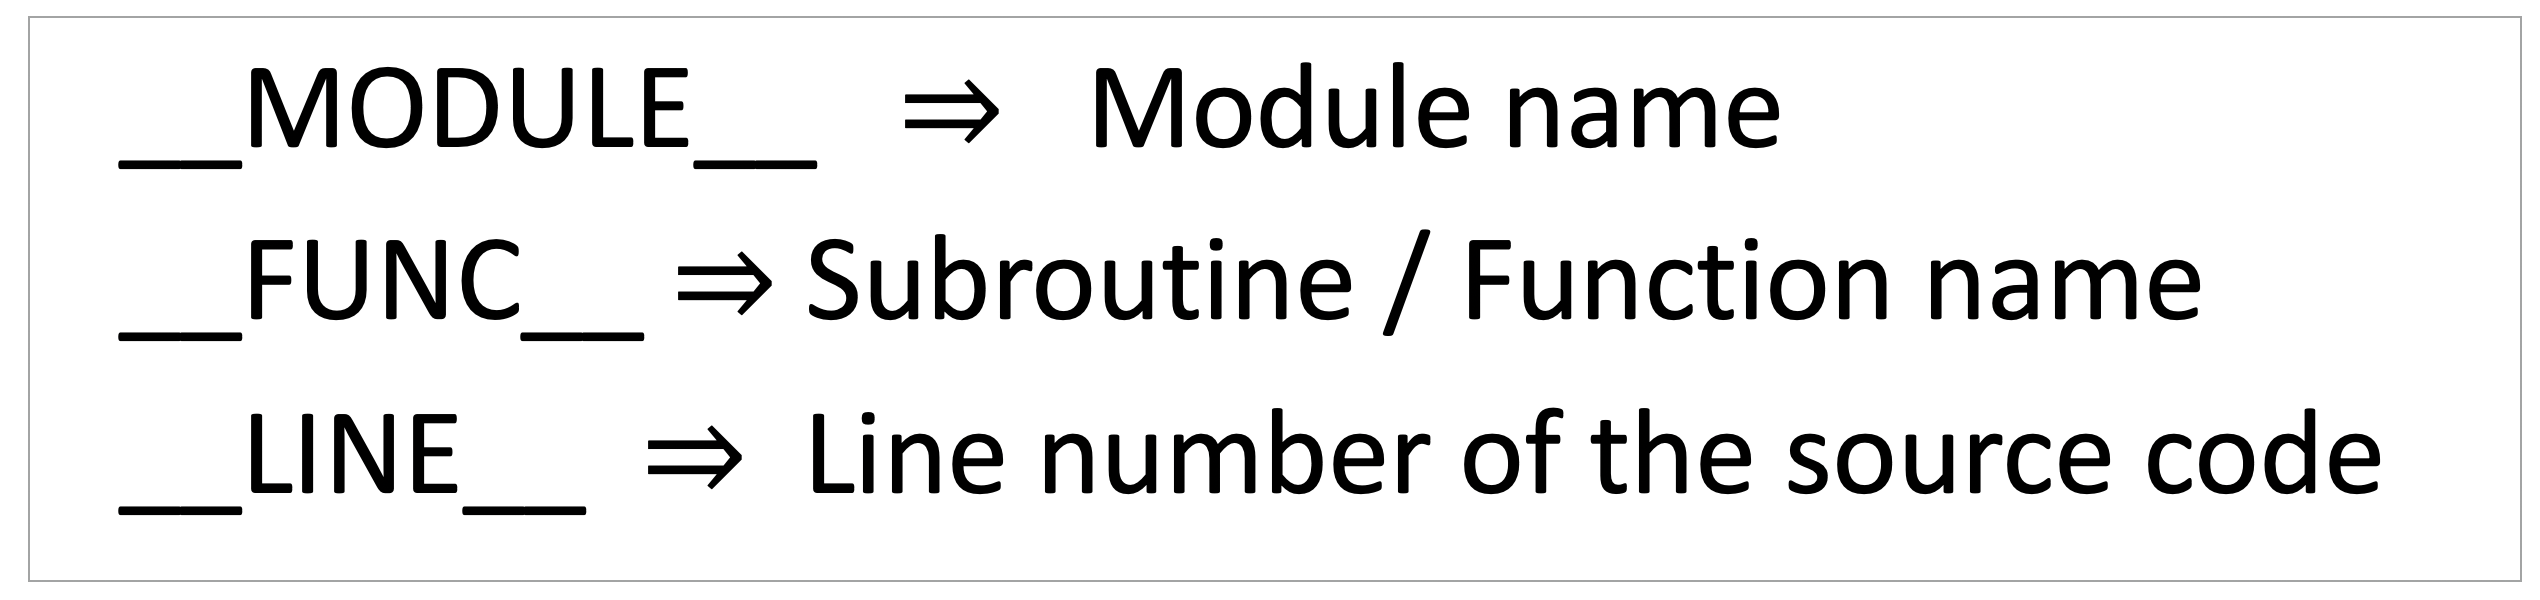
\includegraphics[height=0.5\textheight,width=1.0\hsize,angle=0,keepaspectratio]{./Image/macros4.png}
\caption{String substitution in source code} \label{macros}
\end{figure}

\newpage

\subsection{サンプルコード}
最後にeFortranのサンプルコードと変換後の標準Fortranコードを以下に示す(Fig.\ref{sample_e03},Fig.\ref{sample_f90})

\begin{figure}[H]
\centering
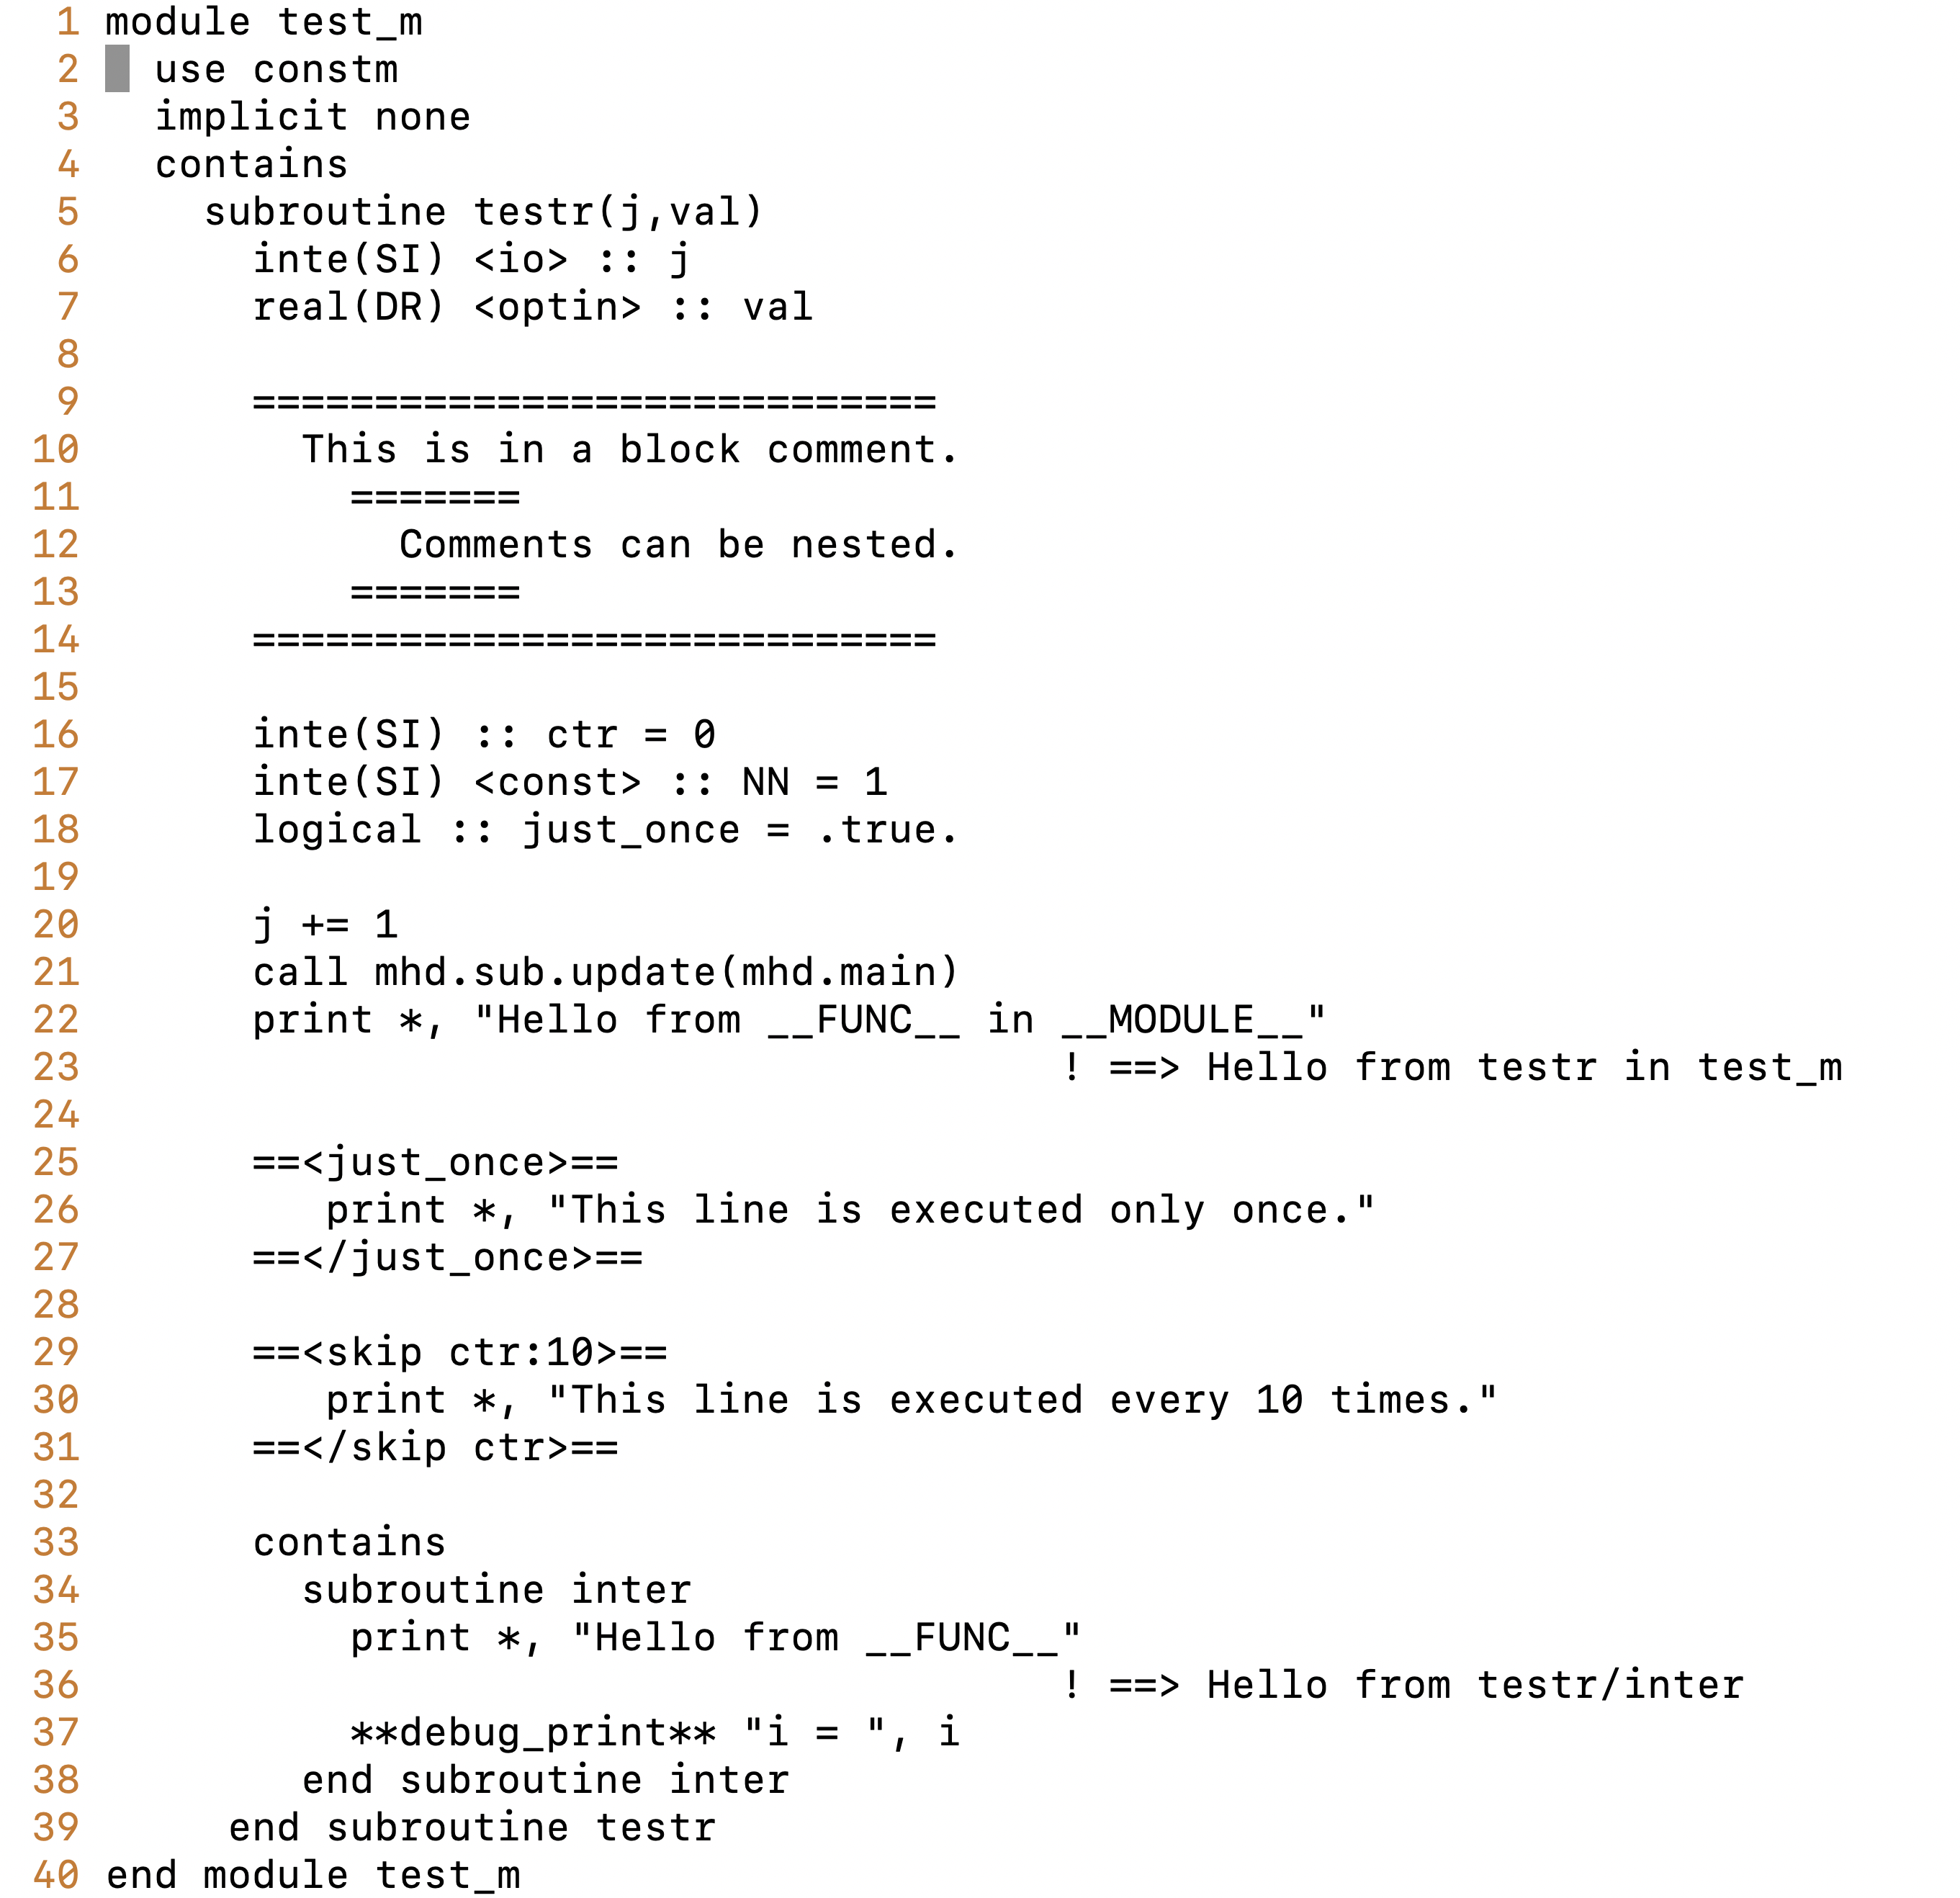
\includegraphics[height=1.0\textheight,width=1.0\hsize,angle=0,keepaspectratio]{./Image/sample2_e03.png}
\caption{Sample eFortran code.} \label{sample_e03}
\end{figure}


\begin{figure}[H]
\centering
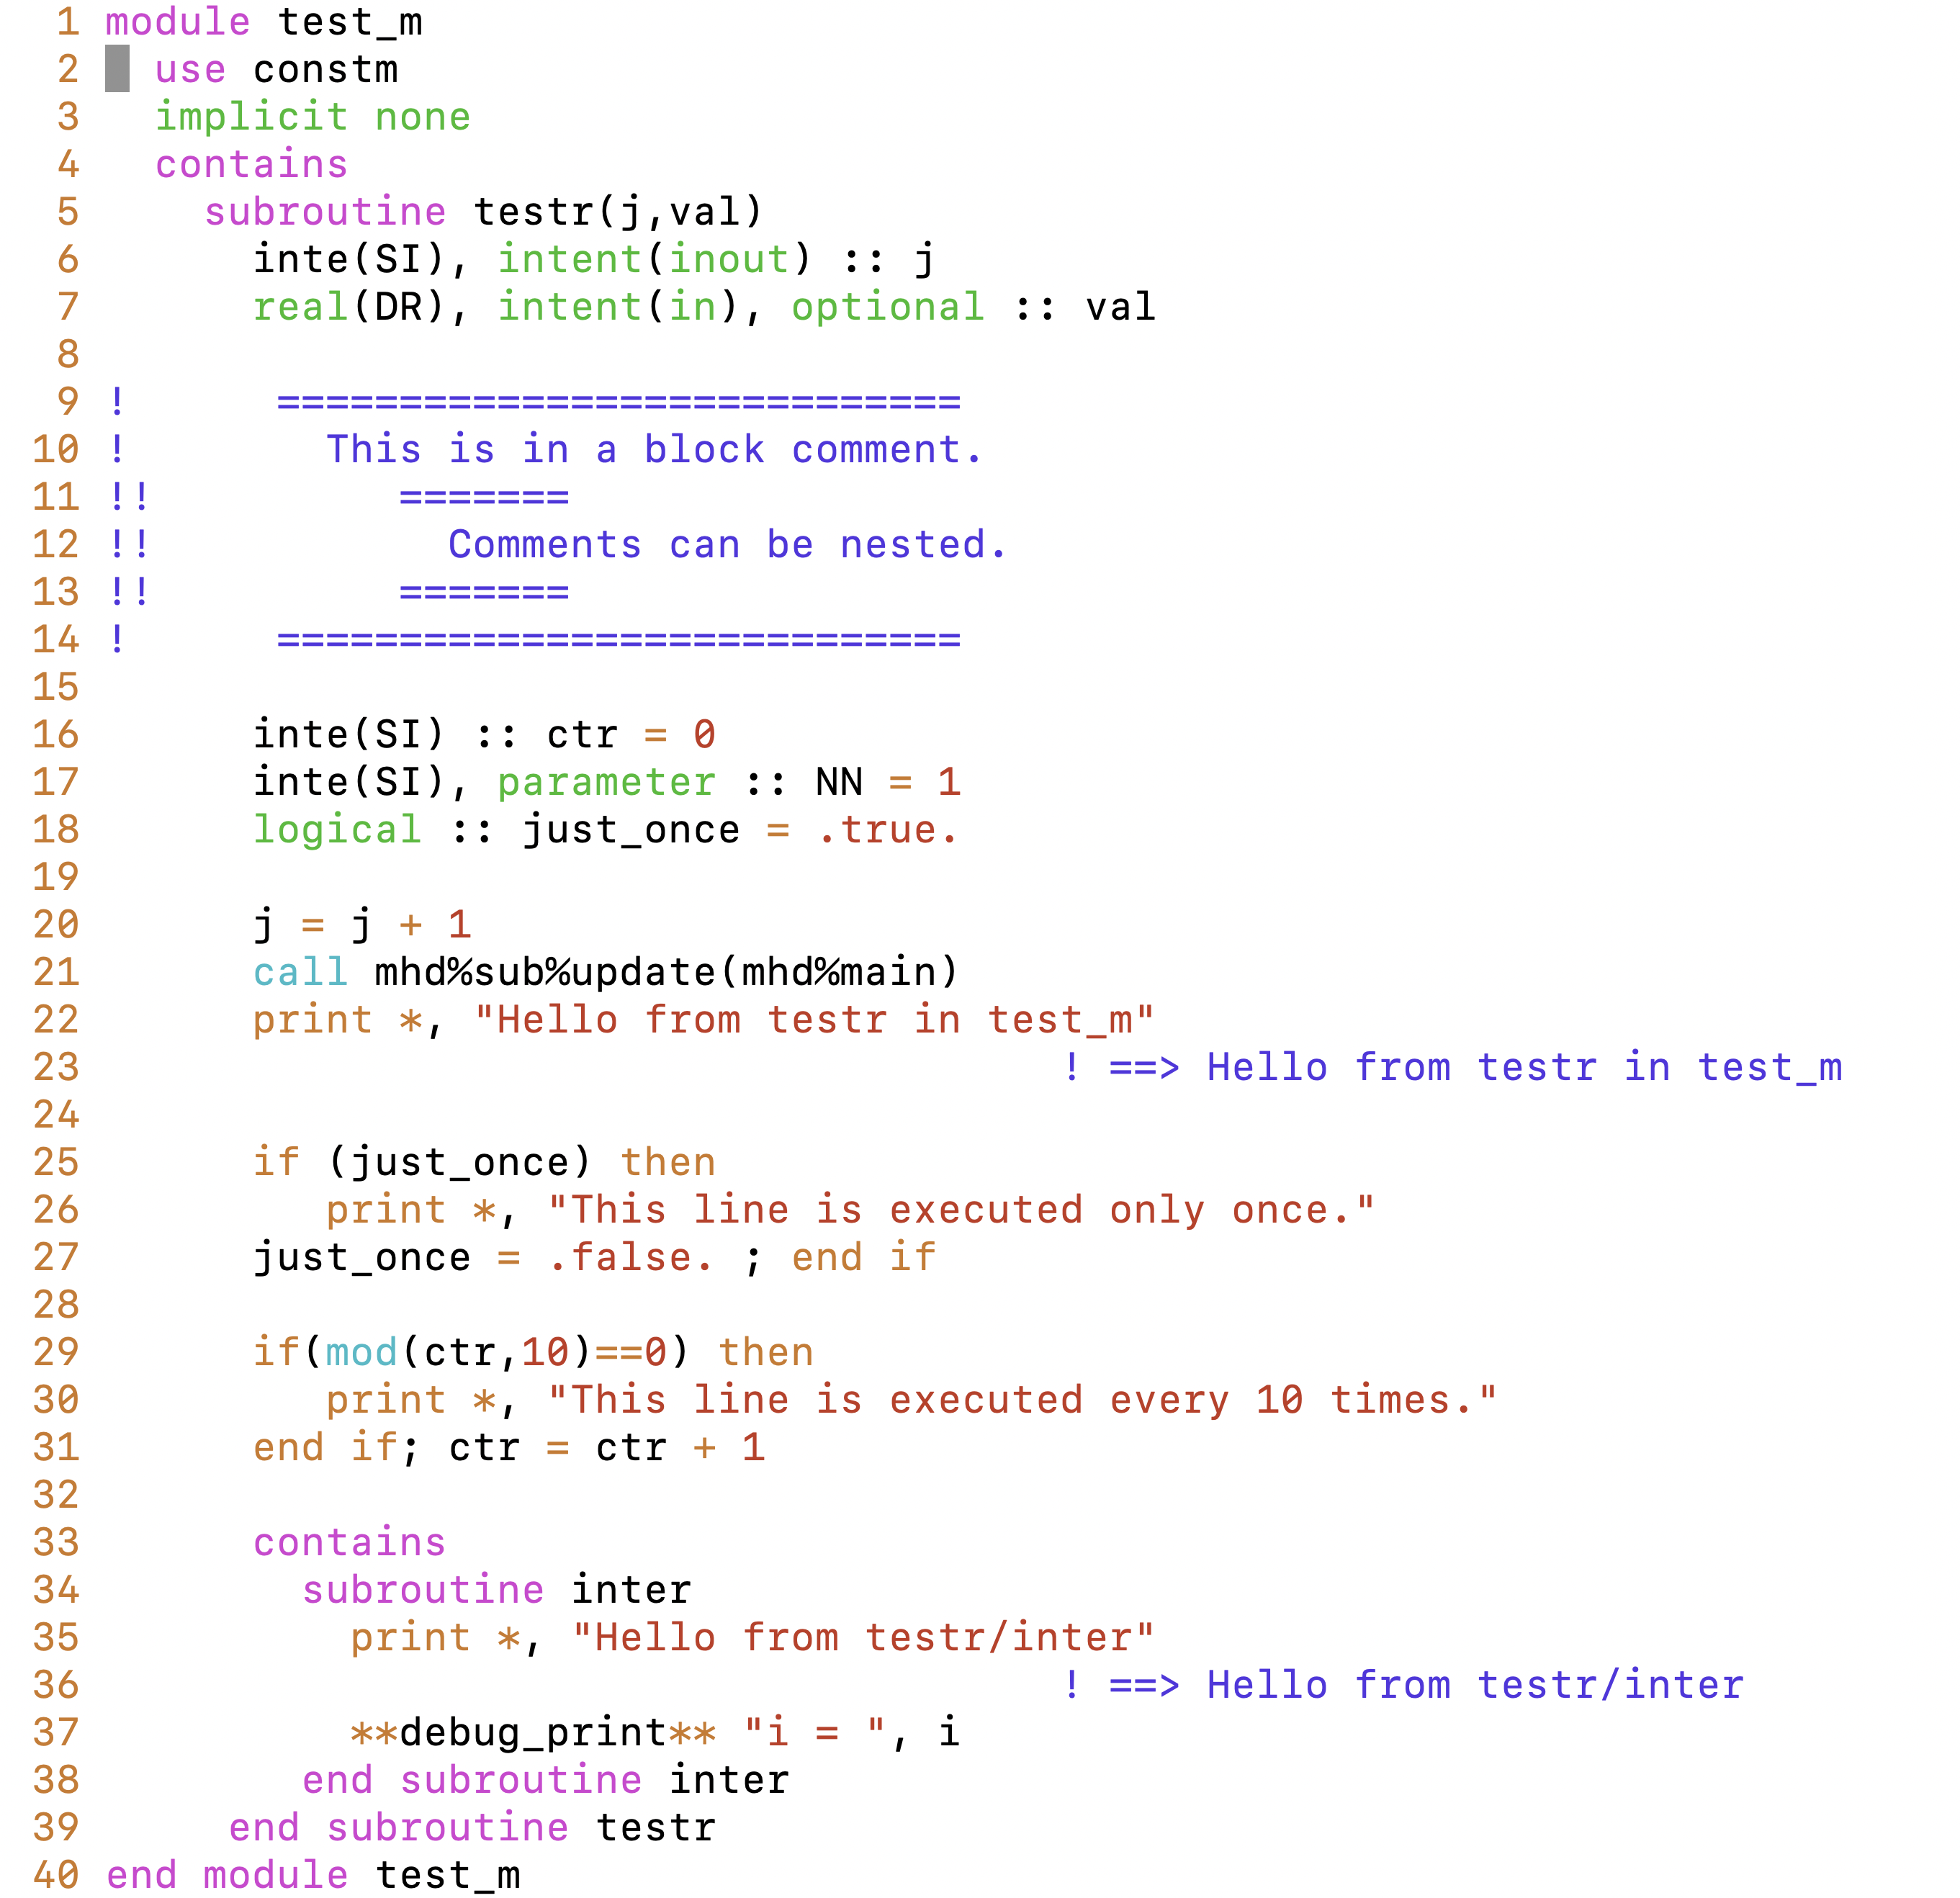
\includegraphics[height=1.0\textheight,width=1.0\hsize,angle=0,keepaspectratio]{./Image/sample2_f90.png}
\caption{Standard Fortran code converted from eFortran} \label{sample_f90}
\end{figure}


%=============================================
\section{計算モデルとコードの実装}

\subsection{計算手法}
Yin--Yang--Zhong格子を用いて単位球体内部(半径$r=1$)でのMHD方程式(式(1)-(4))の数値計算を行う。基本変数を質量流束$\bm f$、ベクトルポテンシャル$\bm{a}$、質量密度$\rho$、圧力$p$の4つとし、計算領域は全球($0 \leq r \leq 1$)とする。離散化の手法として、空間微分は有限差分法の1つである2次精度中心差分法、時間積分は4次ルンゲ=クッタ法を用いた。

\subsection{初期条件}

\subsubsection{圧力・質量密度}
本研究では圧縮性MHD方程式を解く。圧縮性の物理的な効果は可能な限り小さくするために、代表的な流速を$U$、音速を$C$とすると
\begin{equation}
\mathcal{M} = \frac{U}{C}
\end{equation}
で定義されるマッハ数$\mathcal{M}$が最大$\mathcal{O}(10^{-1})$の流れを考える。このとき流速を$\mathcal{O}(10^0)$とすると、音速
\begin{equation}
C = \sqrt{\gamma\frac{p}{\rho}}
\end{equation}
は$\mathcal{O}(10)$程度とする。初期状態において規格化した圧力$p$と質量密度$\rho$は
\begin{eqnarray}
p &=& 100.0, \\
\rho &=& 1.0, 
\end{eqnarray}
とする。

\subsubsection{球面調和関数}
本研究のシミュレーションの初期条件として球面調和関数を用いた。ここではまず、球面調和関数の概要を説明する。

球面調和関数とは球面上の関数$f(\theta,\phi)$を展開するのに便利な特殊関数である。$f(\theta,\phi)$は次式のように球面調和関数$Y_l^m$の線形和で表すことができる:

\begin{equation}
f(\theta,\phi) = \sum_{l=0}^L \sum_{m=-l}^l c_l^m Y_l^m (\theta,\phi)
\end{equation}

ここで、$l,m$はそれぞれ$0\leq |m| \leq l$を満たす整数、$c_l^m$は定数である。球面調和関数はフーリエ級数展開を球面に対応させたものともいえる。以下に$0 \leq l \leq 4$の球面調和関数のボリュームレンダリングをに示す(Fig.\ref{spherical})。緑色は正、赤色は負の領域を表す。
\begin{figure}[H]
\centering
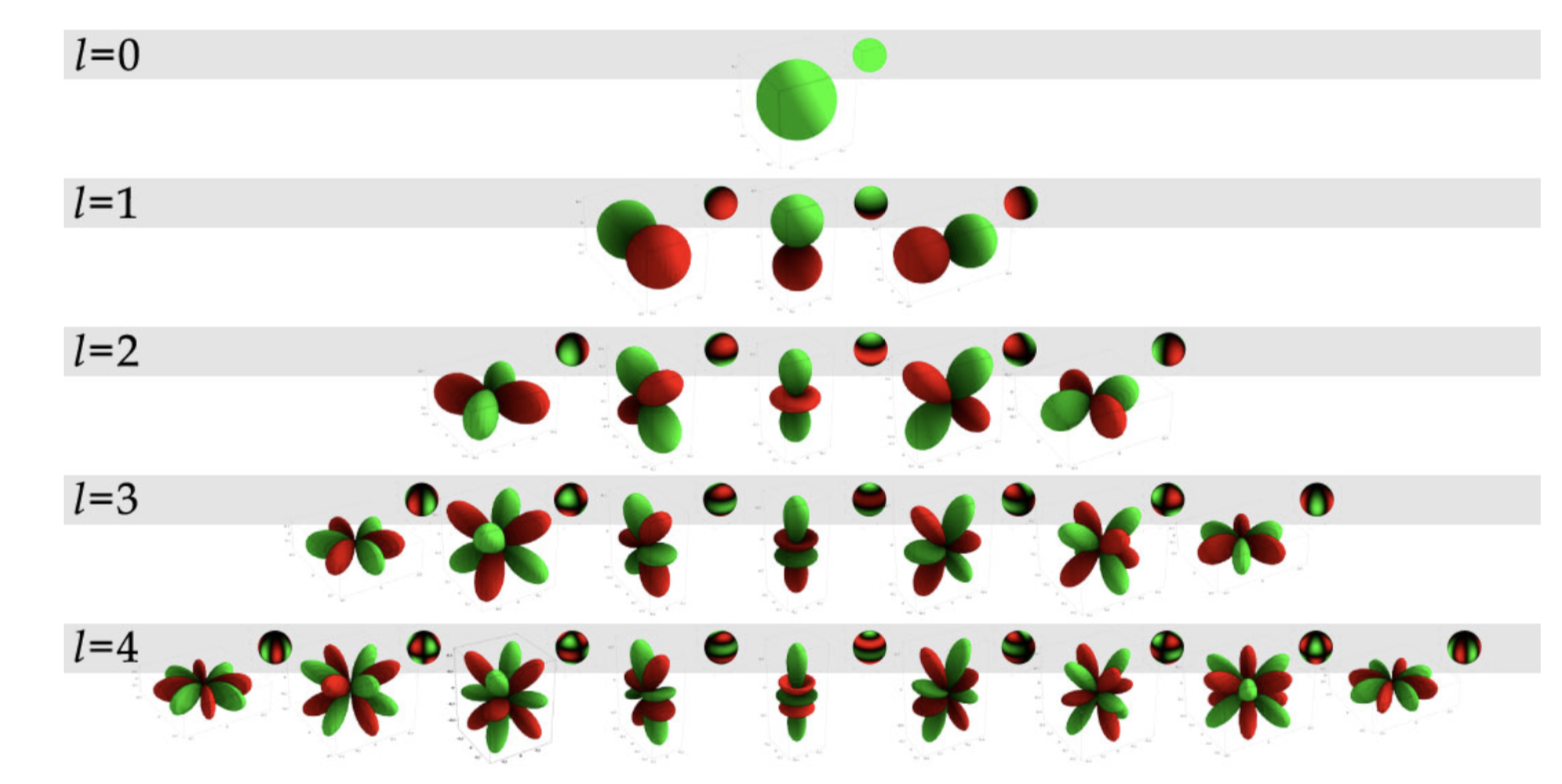
\includegraphics[height=1.0\textheight,width=1.0\hsize,angle=0,keepaspectratio]{./Image/spherical2.png}
\caption{The first 5 Spherical Harmonics plotted ad unsigned spherical functions by distance from the origin. Green are positive values and red are negative.\cite{green2003spherical} } \label{spherical}
\end{figure}


また球面調和関数自体は次式で表される:

\begin{equation}
Y_l^m(\theta,\phi) = \sqrt{\frac{4\pi}{2l+1}\frac{(l+m)!}{(l-m)!}}P_l^m (cos\theta)e^{im\phi}
\end{equation}

ここで、$P_l^m (x)$はルジャンドル陪関数であり緯度方向の展開を表している(ちなみに$e^{im\phi}$は経度方向の展開を表す)。

本研究のシミュレーションではこの球面調和関数の$(l,m)=(3,1),(3,2),(3,3)$の3パターンを初期条件として行った。
具体的には初期の磁場のベクトルポテンシャル$\bm a$と質量流速$\bm f$をそれぞれ以下のように設定した。また以下の表(Table.\ref{spherical})は$(l,m)=(3,1),(3,2),(3,3)$のルジャンドル陪関数と球面調和関数を表している。

\begin{equation}
\bm a
=
\begin{pmatrix}
a_r \\ a_\theta \\ a_\phi  
\end{pmatrix} 
=
\begin{pmatrix}
C \times r \times sin^2(\pi r) P_l^m (cos\theta)cos(m\phi) \\ 0 \\ 0 
\end{pmatrix} , 
\end{equation}

\begin{equation}
\bm f = \bm 0
\end{equation}

\begin{table}[H]
\centering
\caption{Associated Legendre polynomials (left), and spherical harmonics (right).} \label{spherical}
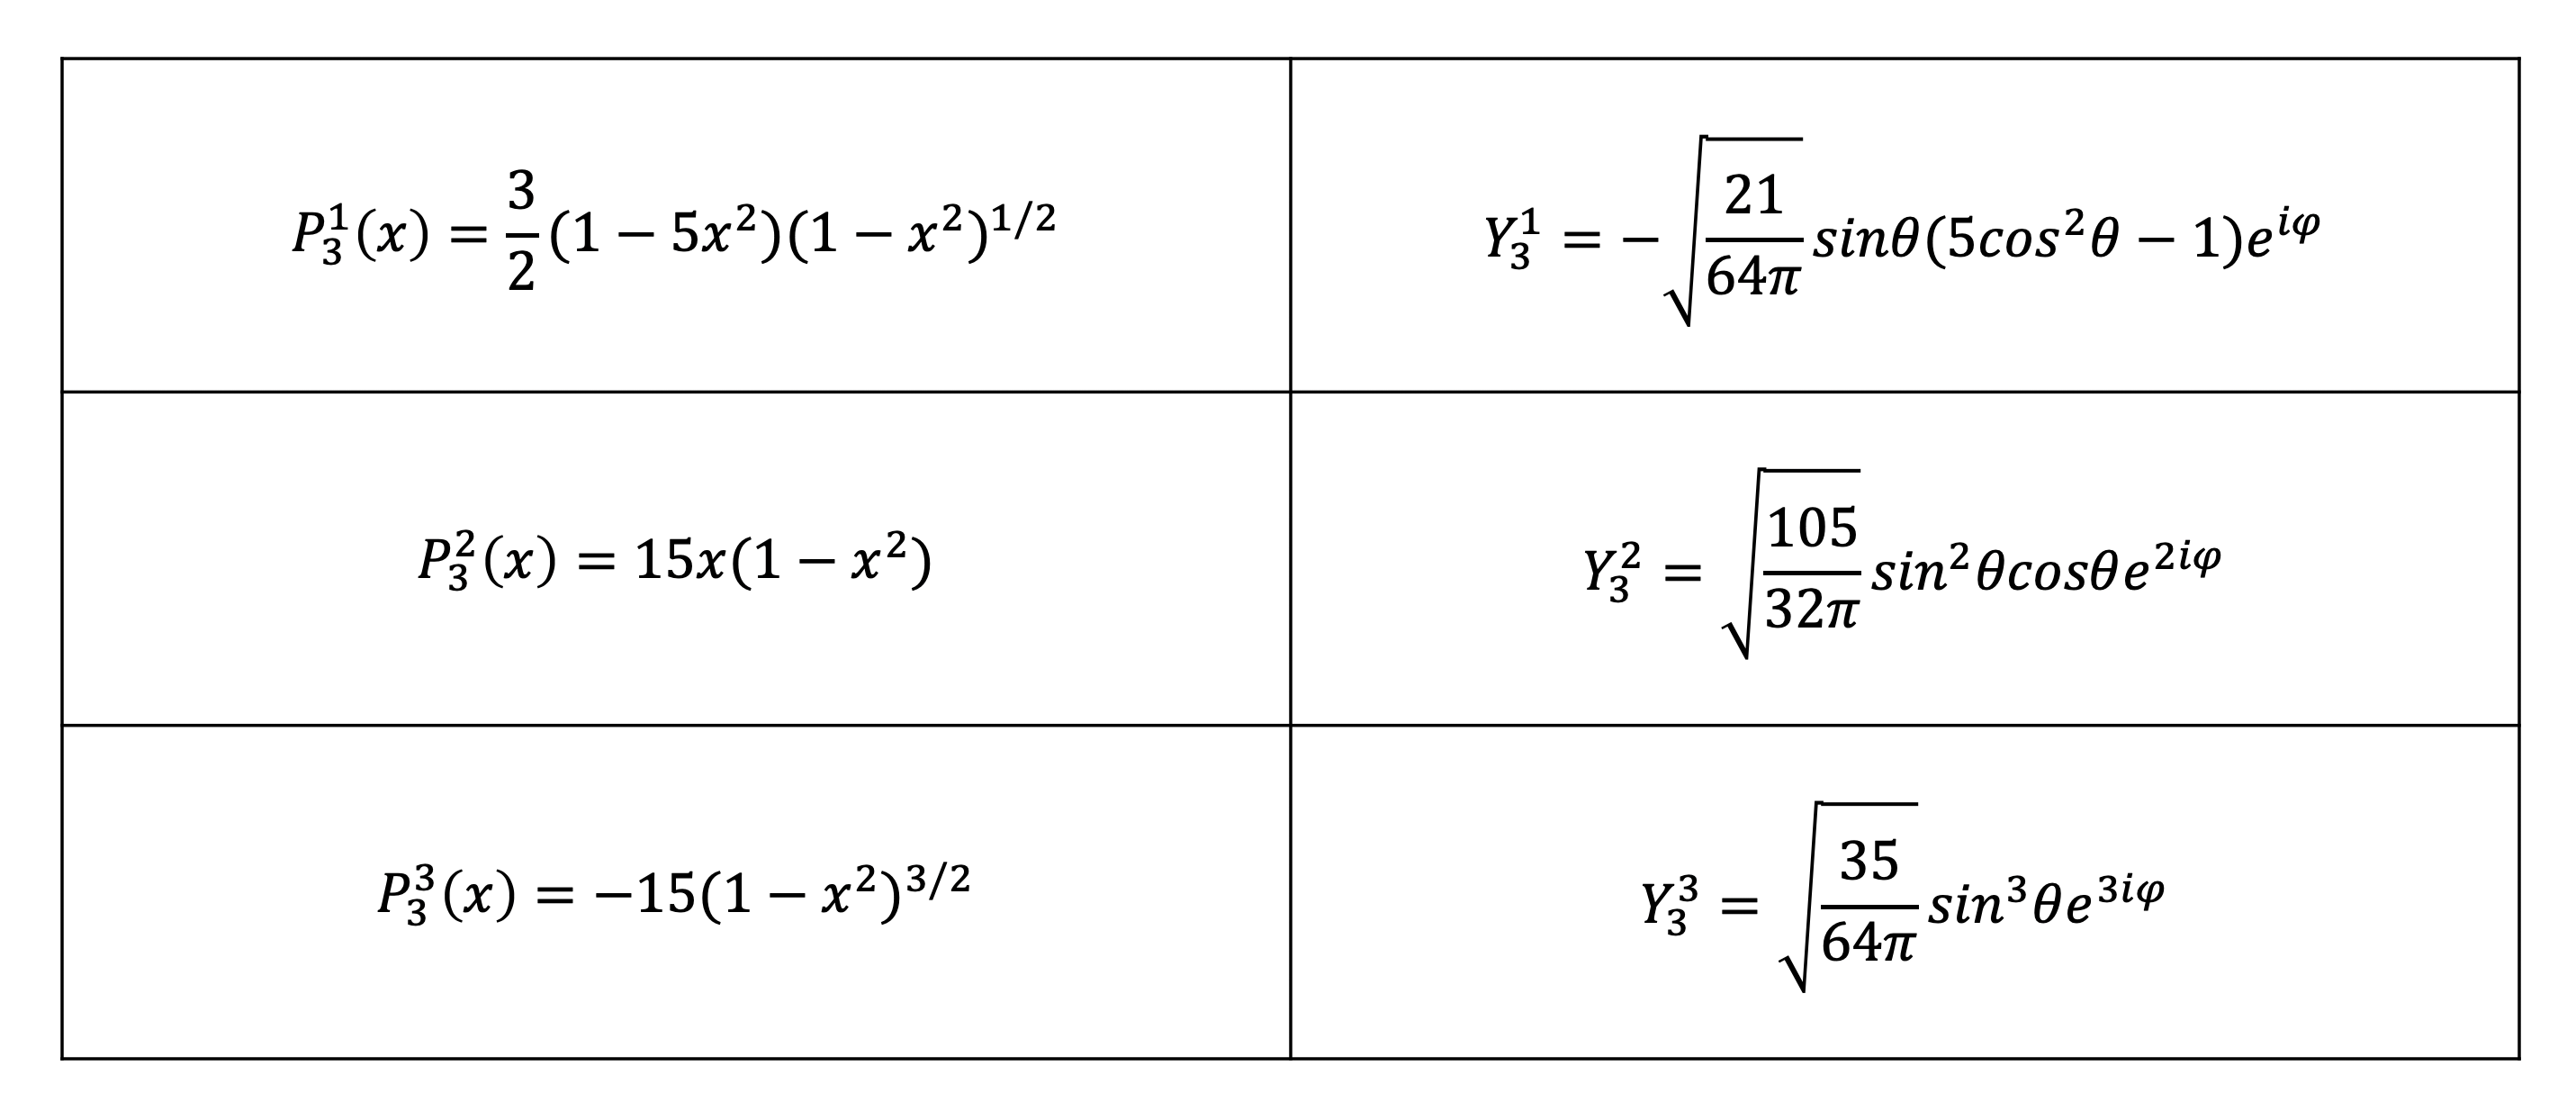
\includegraphics[height=1.0\textheight,width=1.0\hsize,angle=0,keepaspectratio]{./Image/spherical_harmonics3.png}
\end{table}

$C$は定数であり全ての$(l,m)$において$C=0.2$とした。以下に初期磁力線(Fig.\ref{initialMag1})および半径$r=0.9$の経度方向の磁場$b_\phi$の球面分布(Fig.\ref{b0p_L3M1})と球面調和関数展開した時の係数$|c|^2$のグラフ(Fig.\ref{b0p_L3M2})をそれぞれ示す。球面分布の可視化手法にはモルワイデ図法を用いた。
%それぞれ左から$(l,m)=(3,1)$、$(l,m)=(3,2)$、$(l,m)=(3,3)$の磁場を表している。
\begin{figure}[H]
\centering
%\includegraphics[height=1.0\textheight,width=1.0\hsize,angle=0,keepaspectratio]{./Image/initialMag1.png}
%\includegraphics[height=1.0\textheight,width=1.0\hsize,angle=0,keepaspectratio]{./Image/initialMag2.png}
\includegraphics[height=1.0\textheight,width=1.0\hsize,angle=0,keepaspectratio]{./Image/initialMag3.png}
\caption{Initial magnetic field in $(l,m)=(3,1)$(left), $(3,2)$(middle), $(3,3)$(right).  } \label{initialMag1}
\end{figure}

\begin{figure}[H]
\centering
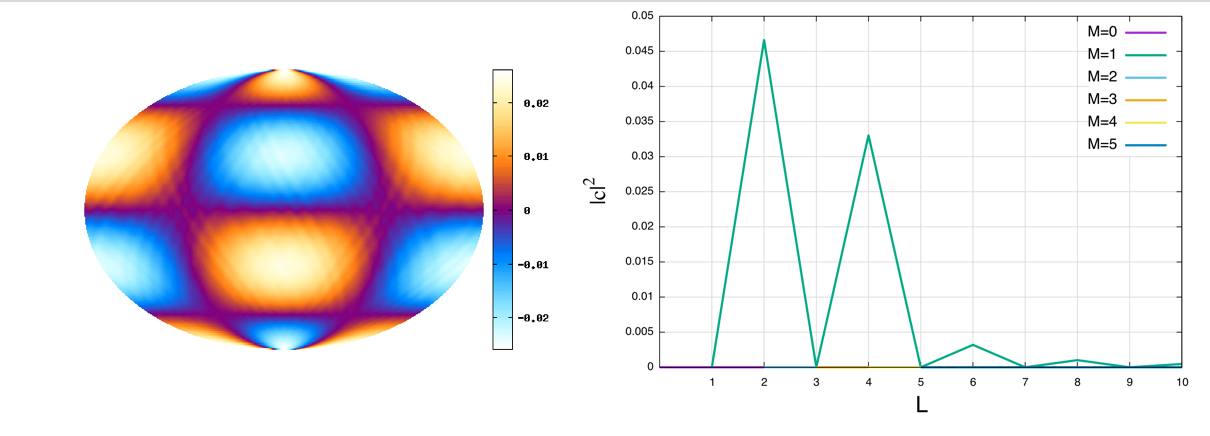
\includegraphics[height=1.0\textheight,width=1.0\hsize,angle=0,keepaspectratio]{./Image/b0p_L3M1.png}
\caption{Snapshots in logitude-latitude Mollwide Projection of initial longitude magnetic field $b_\phi$ (left) and coefficients of spherical harmonics expansion to surface of sphere $r=0.9$ (right) in $(l,m)=(3,1)$.  } \label{b0p_L3M1}
\end{figure}

\begin{figure}[H]
\centering
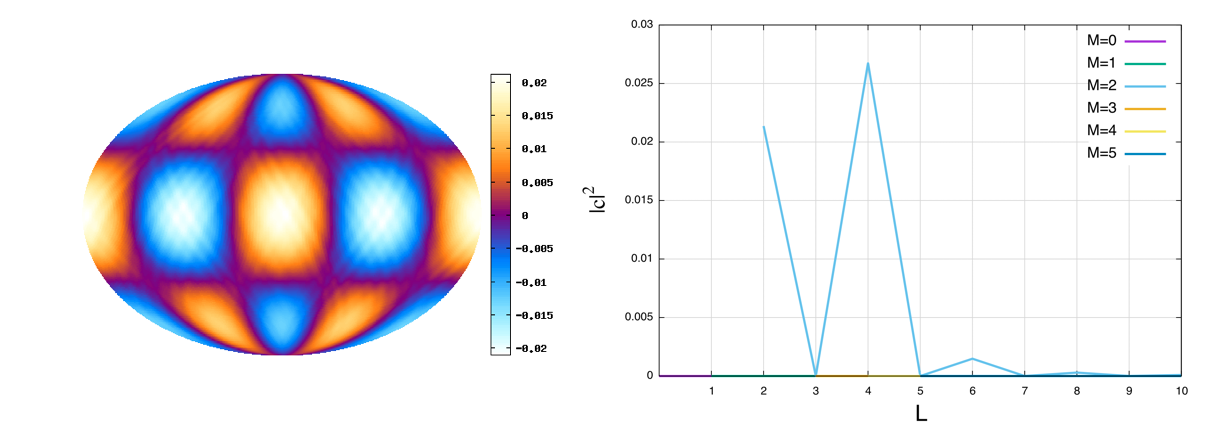
\includegraphics[height=1.0\textheight,width=1.0\hsize,angle=0,keepaspectratio]{./Image/b0p_L3M2.png}
\caption{Snapshots in logitude-latitude Mollwide Projection of initial longitude magnetic field $b_\phi$ (left) and coefficients of spherical harmonics expansion to surface of sphere $r=0.9$ (right) in $(l,m)=(3,2)$.  } \label{b0p_L3M2}
\end{figure}

\begin{figure}[H]
\centering
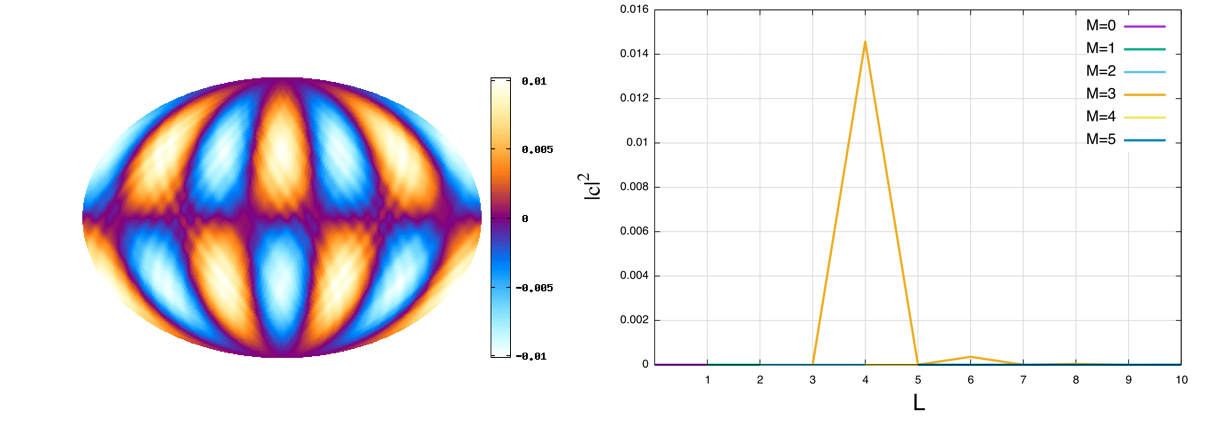
\includegraphics[height=1.0\textheight,width=1.0\hsize,angle=0,keepaspectratio]{./Image/b0p_L3M3.png}
\caption{Snapshots in logitude-latitude Mollwide Projection of initial longitude magnetic field $b_\phi$ (left) and coefficients of spherical harmonics expansion to surface of sphere $r=0.9$ (right) in $(l,m)=(3,3)$.  }\label{b0p_L3M3}
\end{figure}


%\subsubsection{リング状磁場を用いた初期条件}
%続いて、コードの正当性を確認した上で磁場の初期状態に経度方向にのみ磁場が存在するリング状磁場を用いて計算した。Fig.\ref{fig:equat.mag.0000000.+0.000E+00noomega}に初期磁場の赤道断面の様子を、Fig.\ref{fig:initial_mag_12}にそのベクトル図を示す。
%\begin{figure}[H]
%\centering
%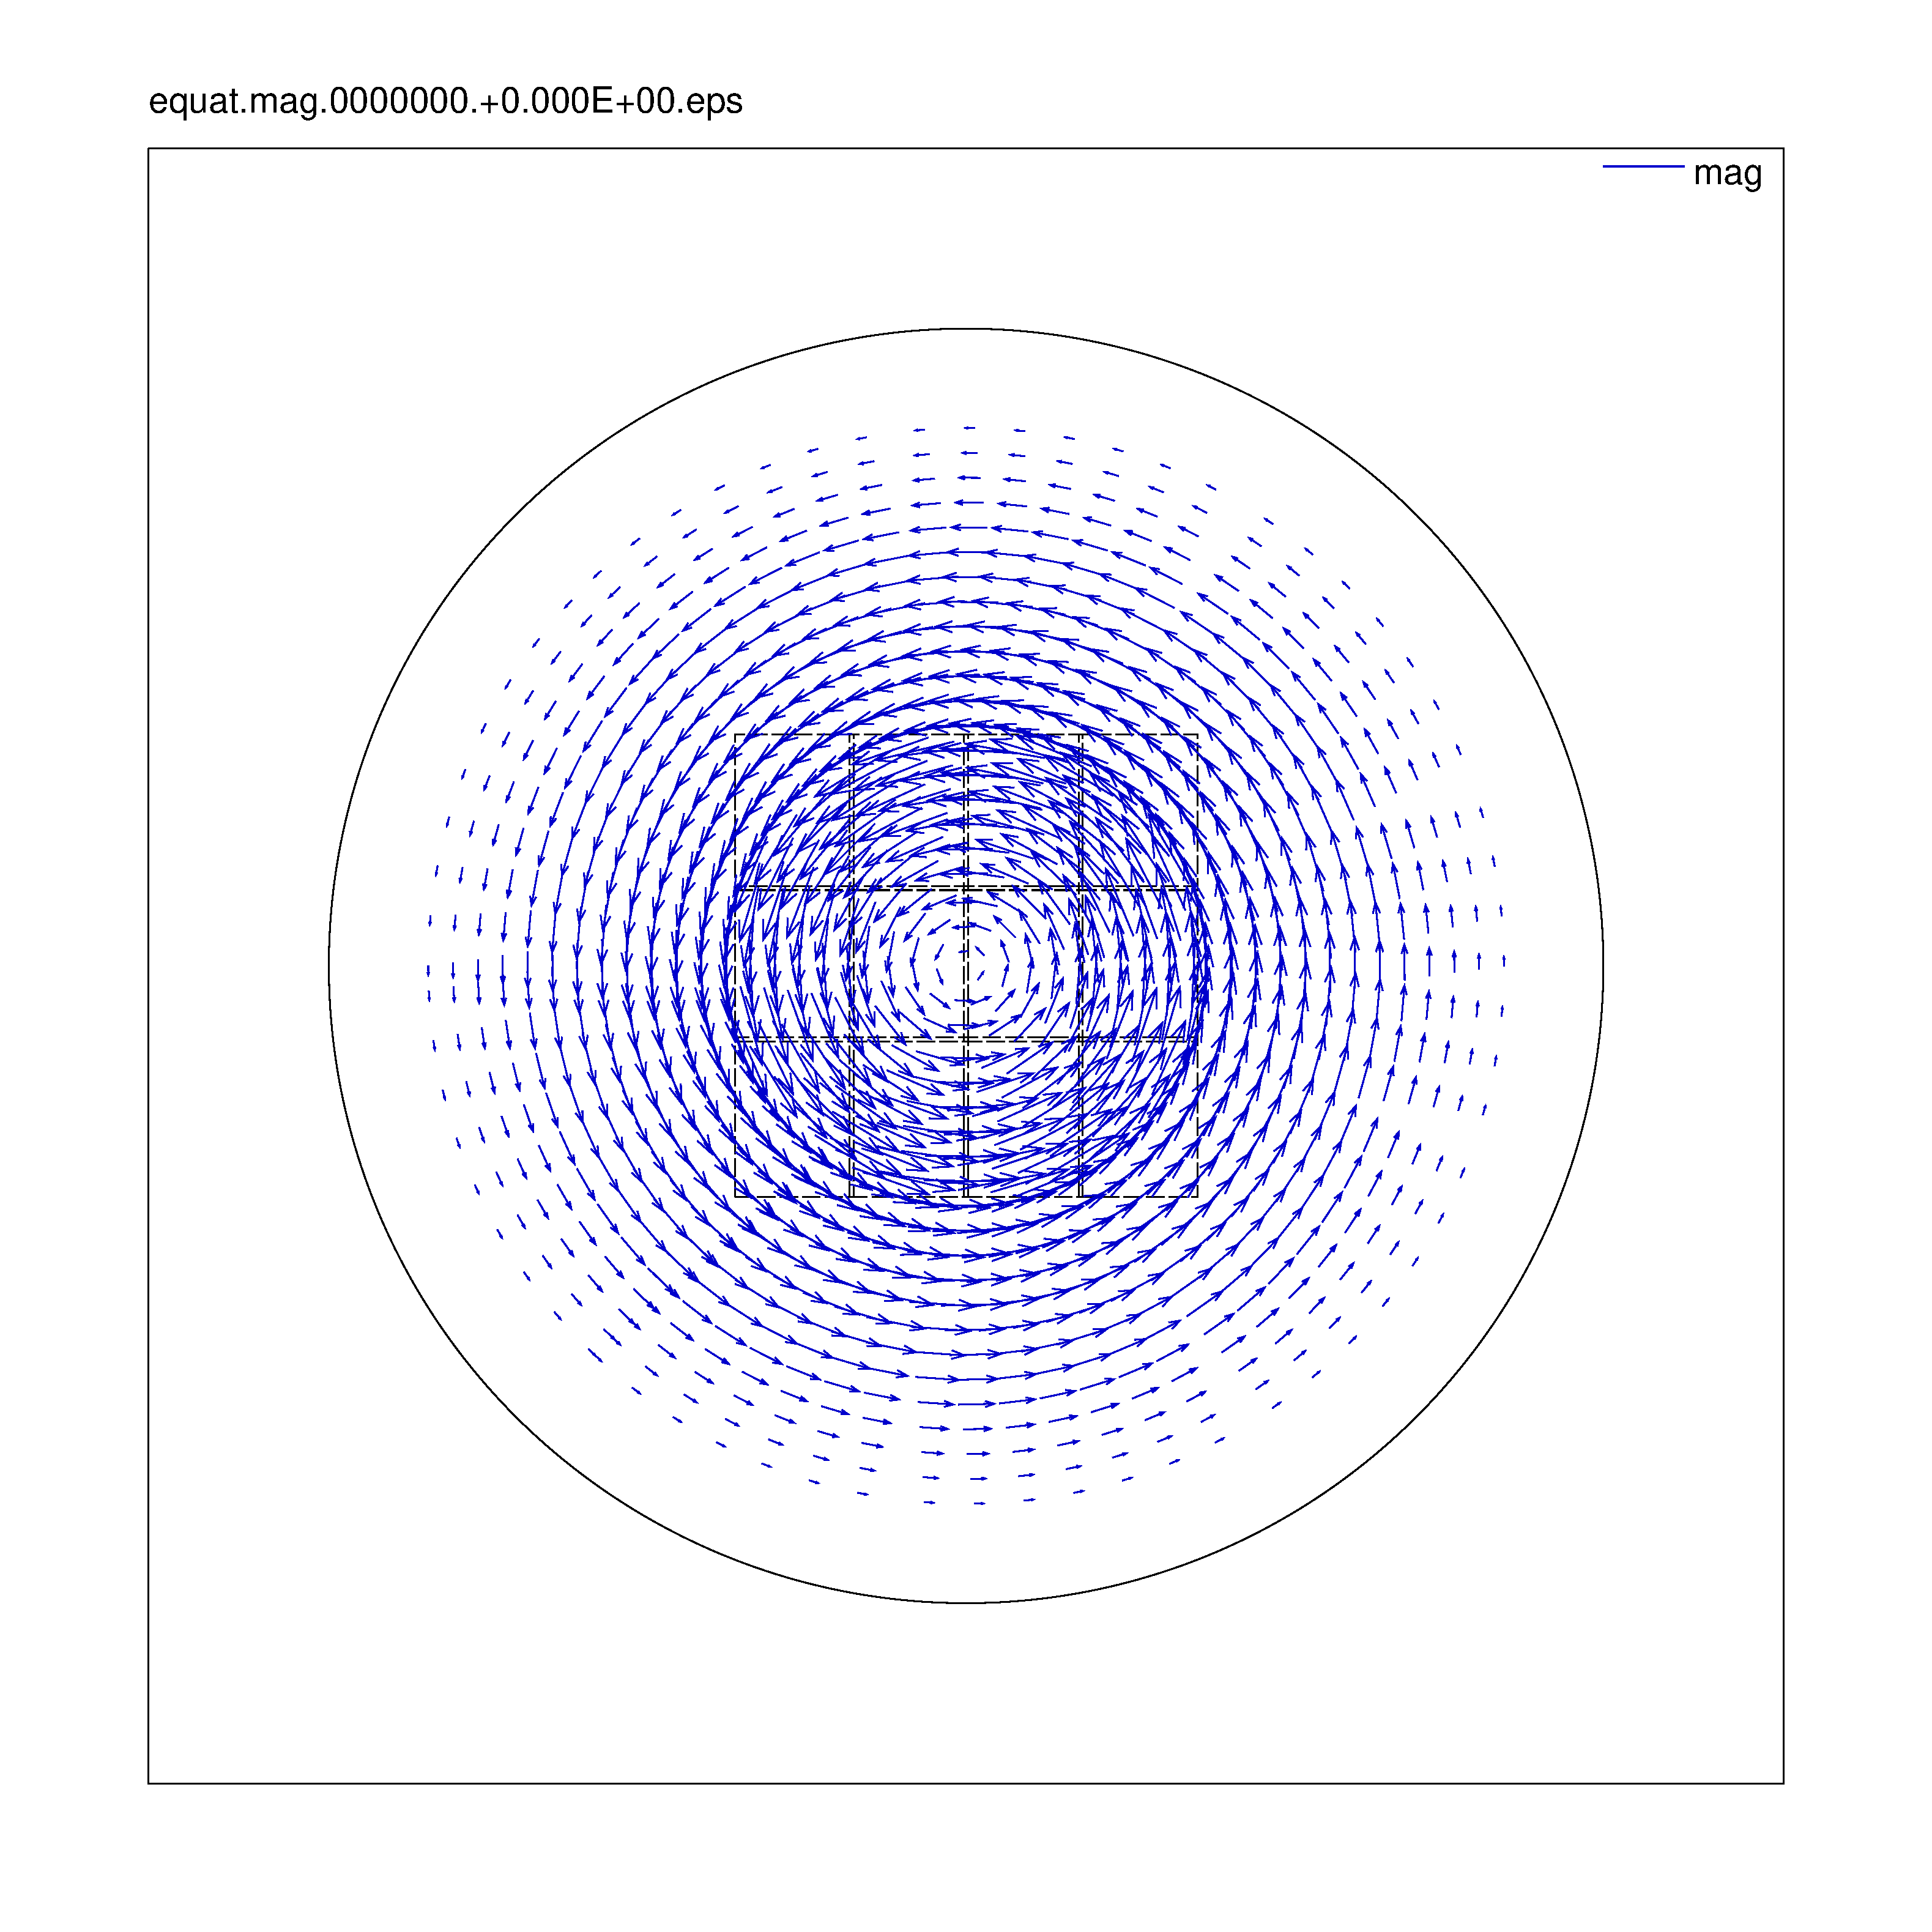
\includegraphics[height=0.5\textheight,width=1.0\hsize,angle=0,keepaspectratio]{./Image/tro_noomega/equat.mag.0000000.+0.000E+00.eps}
%\caption{Initial toroidal magnetic field on the equator.} \label{fig:equat.mag.0000000.+0.000E+00noomega}
%\end{figure}
%\begin{figure}[H]
%\centering
%\includegraphics[height=0.75\textheight,width=1.0\hsize,angle=0,keepaspectratio]{./Image/tro_noomega/init_mag_12.png}
%\caption{Streamline of initial toroidal magnetic field.} \label{fig:initial_mag_12}
%\end{figure}
%このようなリング状磁場を生成するために、磁場のベクトルポテンシャルを
%\begin{eqnarray}
%a_r&=&\alpha\sin^2(\pi r)\cos(\theta), \\
%a_\theta&=&0 , \\
%a_\phi&=&0 , 
%\end{eqnarray}
%と設定した。ここで、$\alpha$は0.1とした。この式は後述の境界条件を満足する。また、初期速度場はゼロとする。


\subsection{境界条件}
本研究では、磁場に関しては完全導体壁境界条件(磁力線が境界を貫かない)、速度場に関してはrigid境界条件(流れがない)、温度に関しては断熱境界条件(熱の出入りがない)を用いた。つまり境界面を$S$、境界面に垂直な単位ベクトルを$\bm n$とすると
\begin{align}
\bm{v} &= \bm{0} \; ({\rm on}\, S), \\
\bm{a} \times \bm{n} &= \bm{0} , \; \frac{\partial a_r}{\partial r} = 0 \; ({\rm on}\, S), \\
\frac{\partial T}{\partial r} &= 0 \; \Leftrightarrow \; \frac{\partial}{\partial r}\left(\frac{p}{\rho}\right) = 0 \; (\because p=\rho T) \; ({\rm on}\, S),  
\end{align}
を意味する。

\subsection{パラメータ設定}
粘性係数$\mu$、電気抵抗$\eta$、熱拡散率$\kappa$はそれぞれ空間的に一様であり規格化された値とする。全ての初期条件で$\mu=1.0\times10^{-4},\eta=1.0\times10^{-4},\kappa=1.0\times10^{-4}$と設定した。
計算の空間解像度は、すべての場合においてYin--Yang格子は動径方向に201、緯度方向に204、経度方向に608,、Zhong格子はx,y,z方向にそれぞれ222である。計算機は地球シミュレータ(NEC SX-ACE, JAMSTEC)を使用した。また3次元可視化ツールとしてParaviewを用いた。

\subsection{eFortran版球MHDコードの概観}
本研究のシミュレーションコードの実装にあたって、eFortranを使用した。ここではそのプログラムコードの概観について説明する。


%\begin{itemize}
 % \renewcommand{\labelitemi}{-}
 % \item main.e03:メインモジュール
  %\item constants.e03:定数モジュール。MHD方程式を解くための定数を定義している。
  %\item cores.e03:Yin--Yang--Zhong格子モジュール。Yin--Yang--Zhongそれぞれの格子内でMHD方程式を解く。
  %\item diagnosis.e03:診断モジュール。数値的なエラーが見つかればプログラムを終了させる。
  %\item ut.e03:ユーリティモジュール。標準出力や型変換などを扱う。
  %\item mpiut.e03:MPIユーティリティモジュール。本シミュレーションはMPIを用いて並列計算をしている。
  %\item namelist.e03:ユーザーがシミュレーションごとに定義する定数が書かれたファイルを読み込むモジュール。
  %\item ppdata.e03:データ出力モジュール。MHDシミュレーションで得られた生データを出力する。
  %\item turtle.e03:2次元可視化モジュール。MHDデータを等高線やベクトルを使って可視化表現する。
%\end{itemize}

\begin{description}
  \item[main.e03]\mbox{}\\
  メインモジュール
  \item[constants.e03]\mbox{}\\
  定数モジュール。MHD方程式を解くための定数を定義している。
  \item[cores.e03]\mbox{}\\
  Yin--Yang--Zhong格子モジュール。Yin--Yang--Zhongそれぞれの格子内でMHD方程式を解く。
  \item [diagnosis.e03]\mbox{}\\
  診断モジュール。数値的なエラーが見つかればプログラムを終了させる。
  \item [ut.e03]\mbox{}\\
  ユーリティモジュール。標準出力や型変換などを扱う。
  \item [mpiut.e03]\mbox{}\\
  MPIユーティリティモジュール。本シミュレーションはMPIを用いて並列計算をしている。
  \item [namelist.e03]\mbox{}\\
  ユーザーがシミュレーションごとに定義する定数が書かれたファイルを読み込むモジュール。
  \item [ppdata.e03]\mbox{}\\
  データ出力モジュール。MHDシミュレーションで得られた生データを出力する。
  \item [turtle.e03]\mbox{}\\
  2次元可視化モジュール。MHDデータを等高線やベクトルを使って可視化表現する。
\end{description}



%=============================================
\section{シミュレーション結果}
%=============================================
%=============================================

\subsection{エネルギーのグラフ}
以下に球面調和関数$Y_l^m$の
\begin{description}
\item{(a)} $(l,m)=(3,1)$
\item{(b)} $(l,m)=(3,2)$
\item{(c)} $(l,m)=(3,3)$
\end{description}
%それぞれの運動エネルギーおよび磁気エネルギーのグラフを示す(Fig.\ref{L3M1_graph}-\ref{L3M3_graph})。なおグラフ化ツールにはgnuplotを用いた。
それぞれの場合における全運動エネルギーおよび全磁気エネルギーのグラフを示す(Fig.\ref{L3M1_graph}-\ref{L3M3_graph})。ここで球領域$V$内の全運動エネルギー$E_{kin}$と全磁気エネルギー$E_{mag}$はそれぞれ次式で表される:
\begin{eqnarray}
E_{kin} &=& \int_V \frac{1}{2} \rho \bm v^2 dV, \\
E_{mag} &=& \int_V \frac{1}{2} \bm b^2 dV
\end{eqnarray}
なおグラフ化ツールにはgnuplotを用いた。
%\begin{figure}[H]
%\centering
%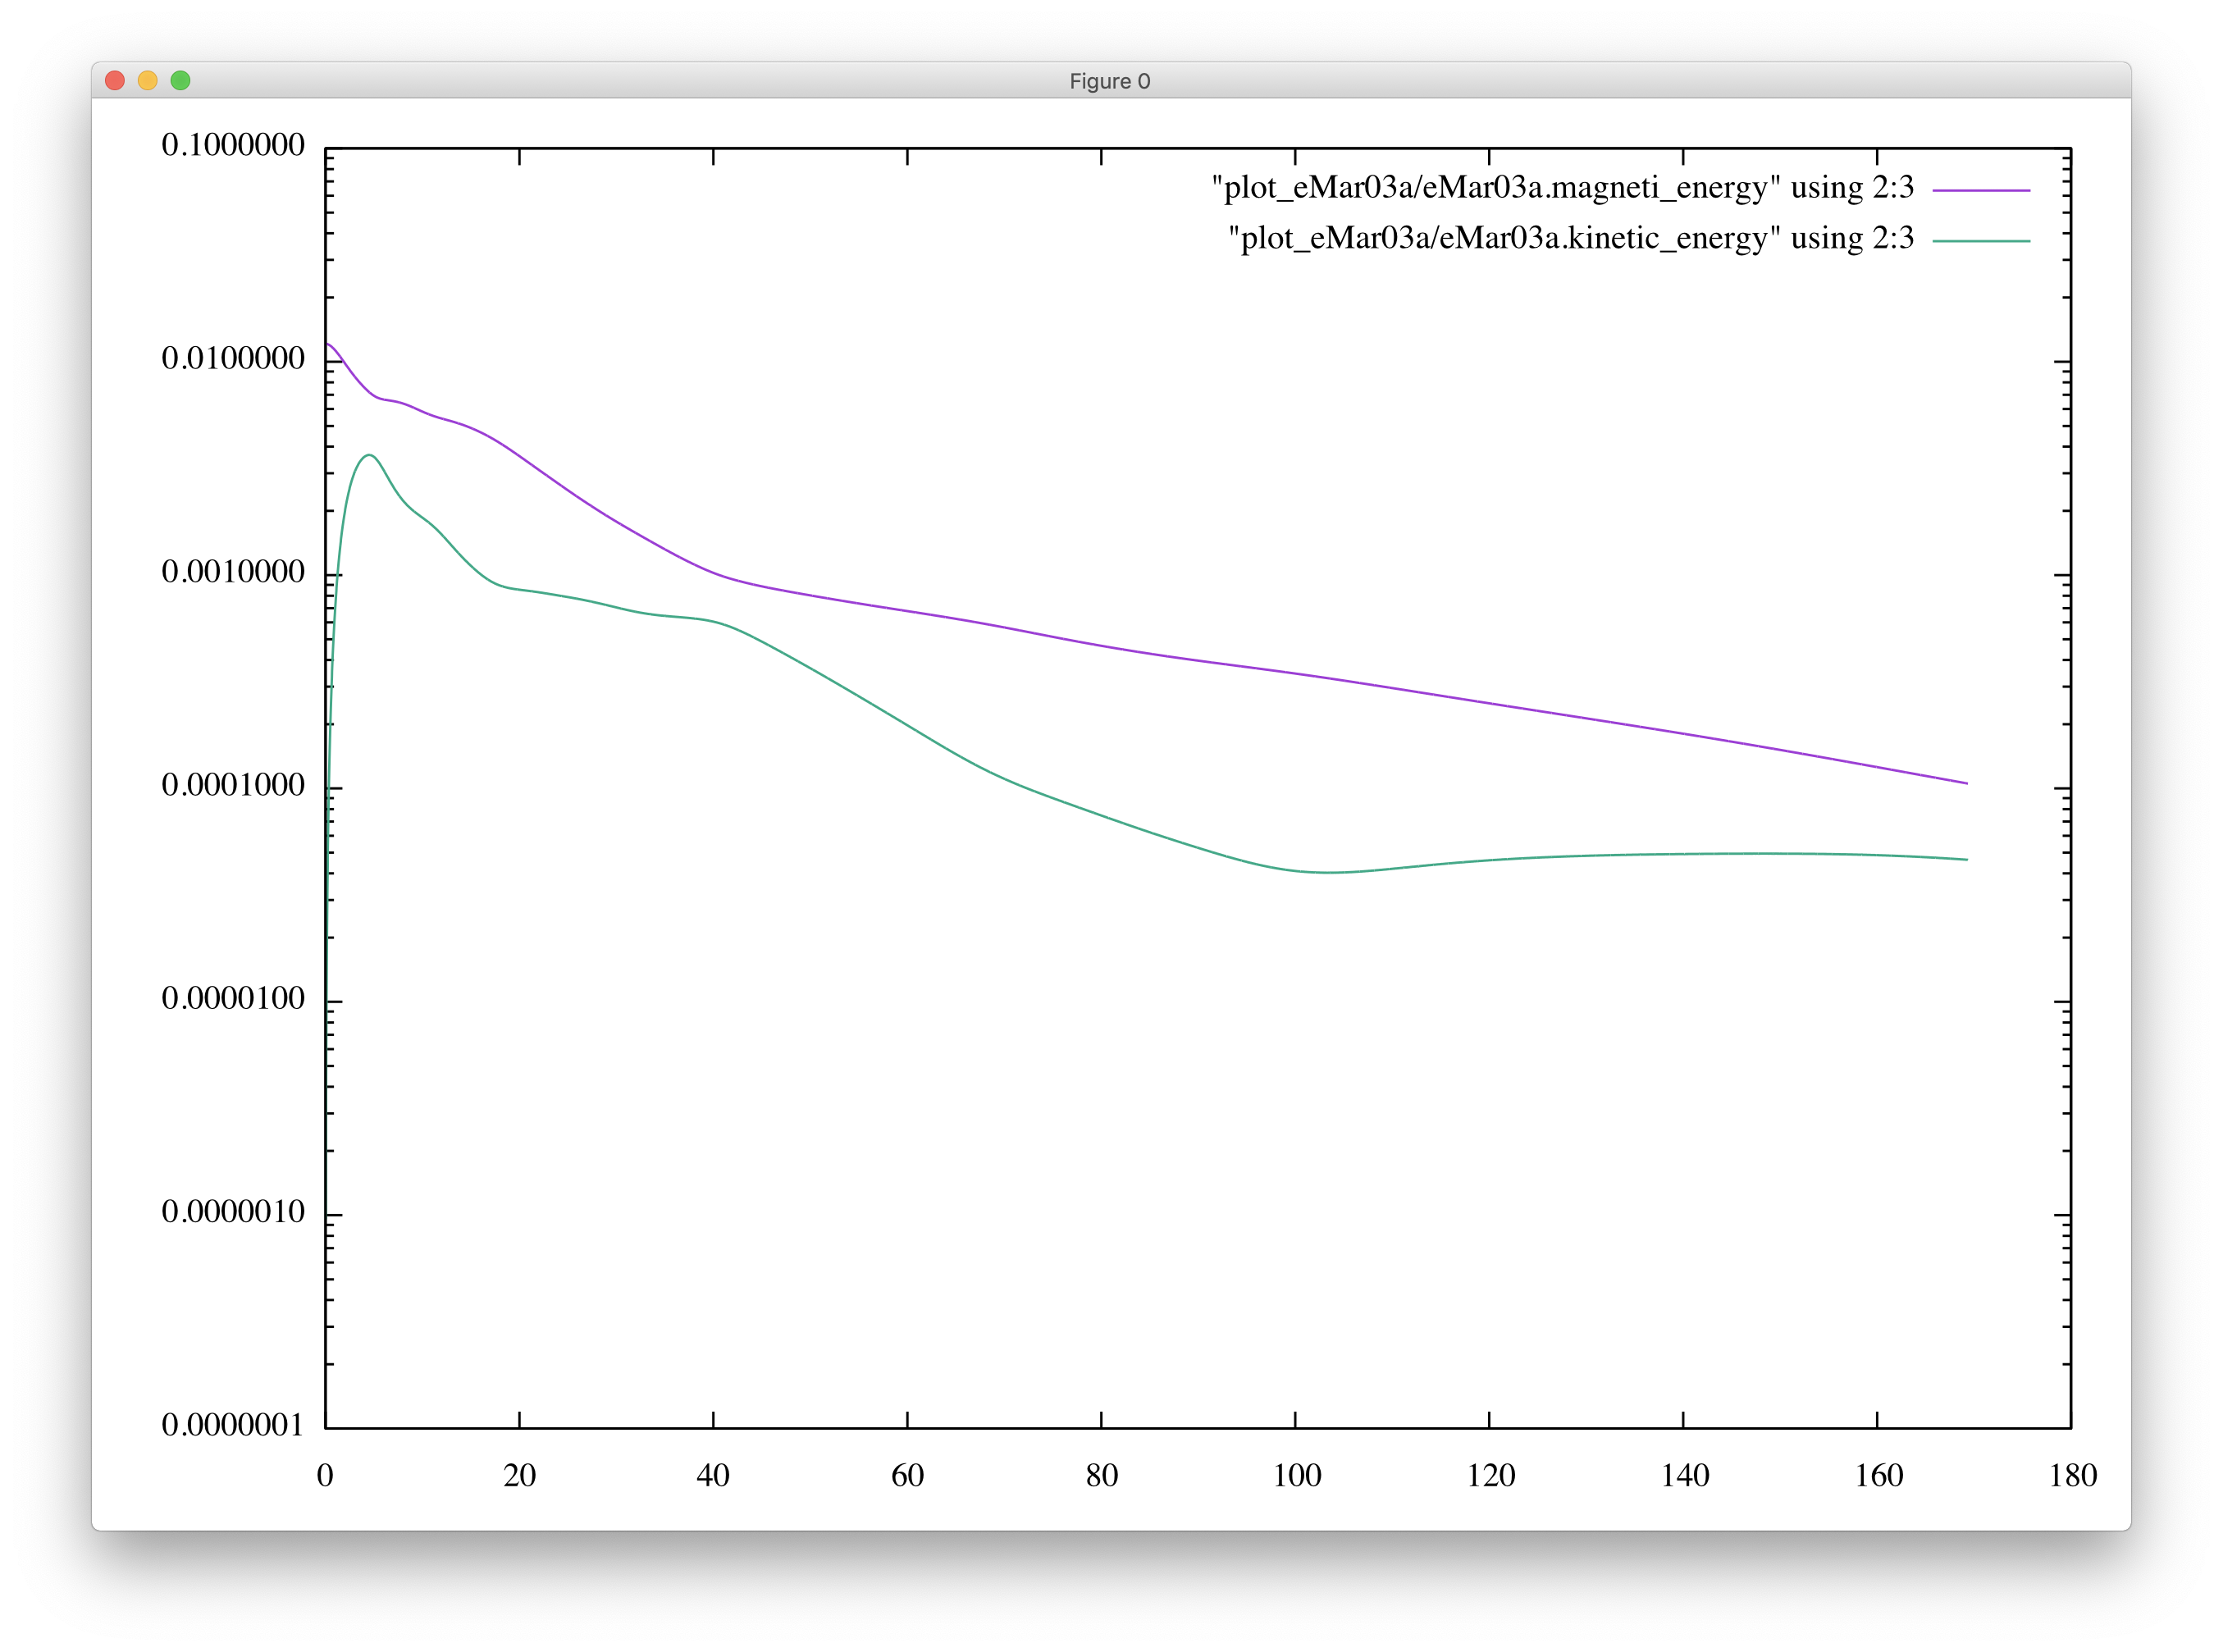
\includegraphics[height=0.5\textheight,width=0.7\hsize,angle=0,keepaspectratio]{./Image/L3M1_graph.png}
%\caption{Relaxation of total magnetic(purple line) and flow(green line) energy in $(l,m)=(3,1)$.} \label{L3M1_graph}
%\end{figure}
%\begin{figure}[H]
%\centering
%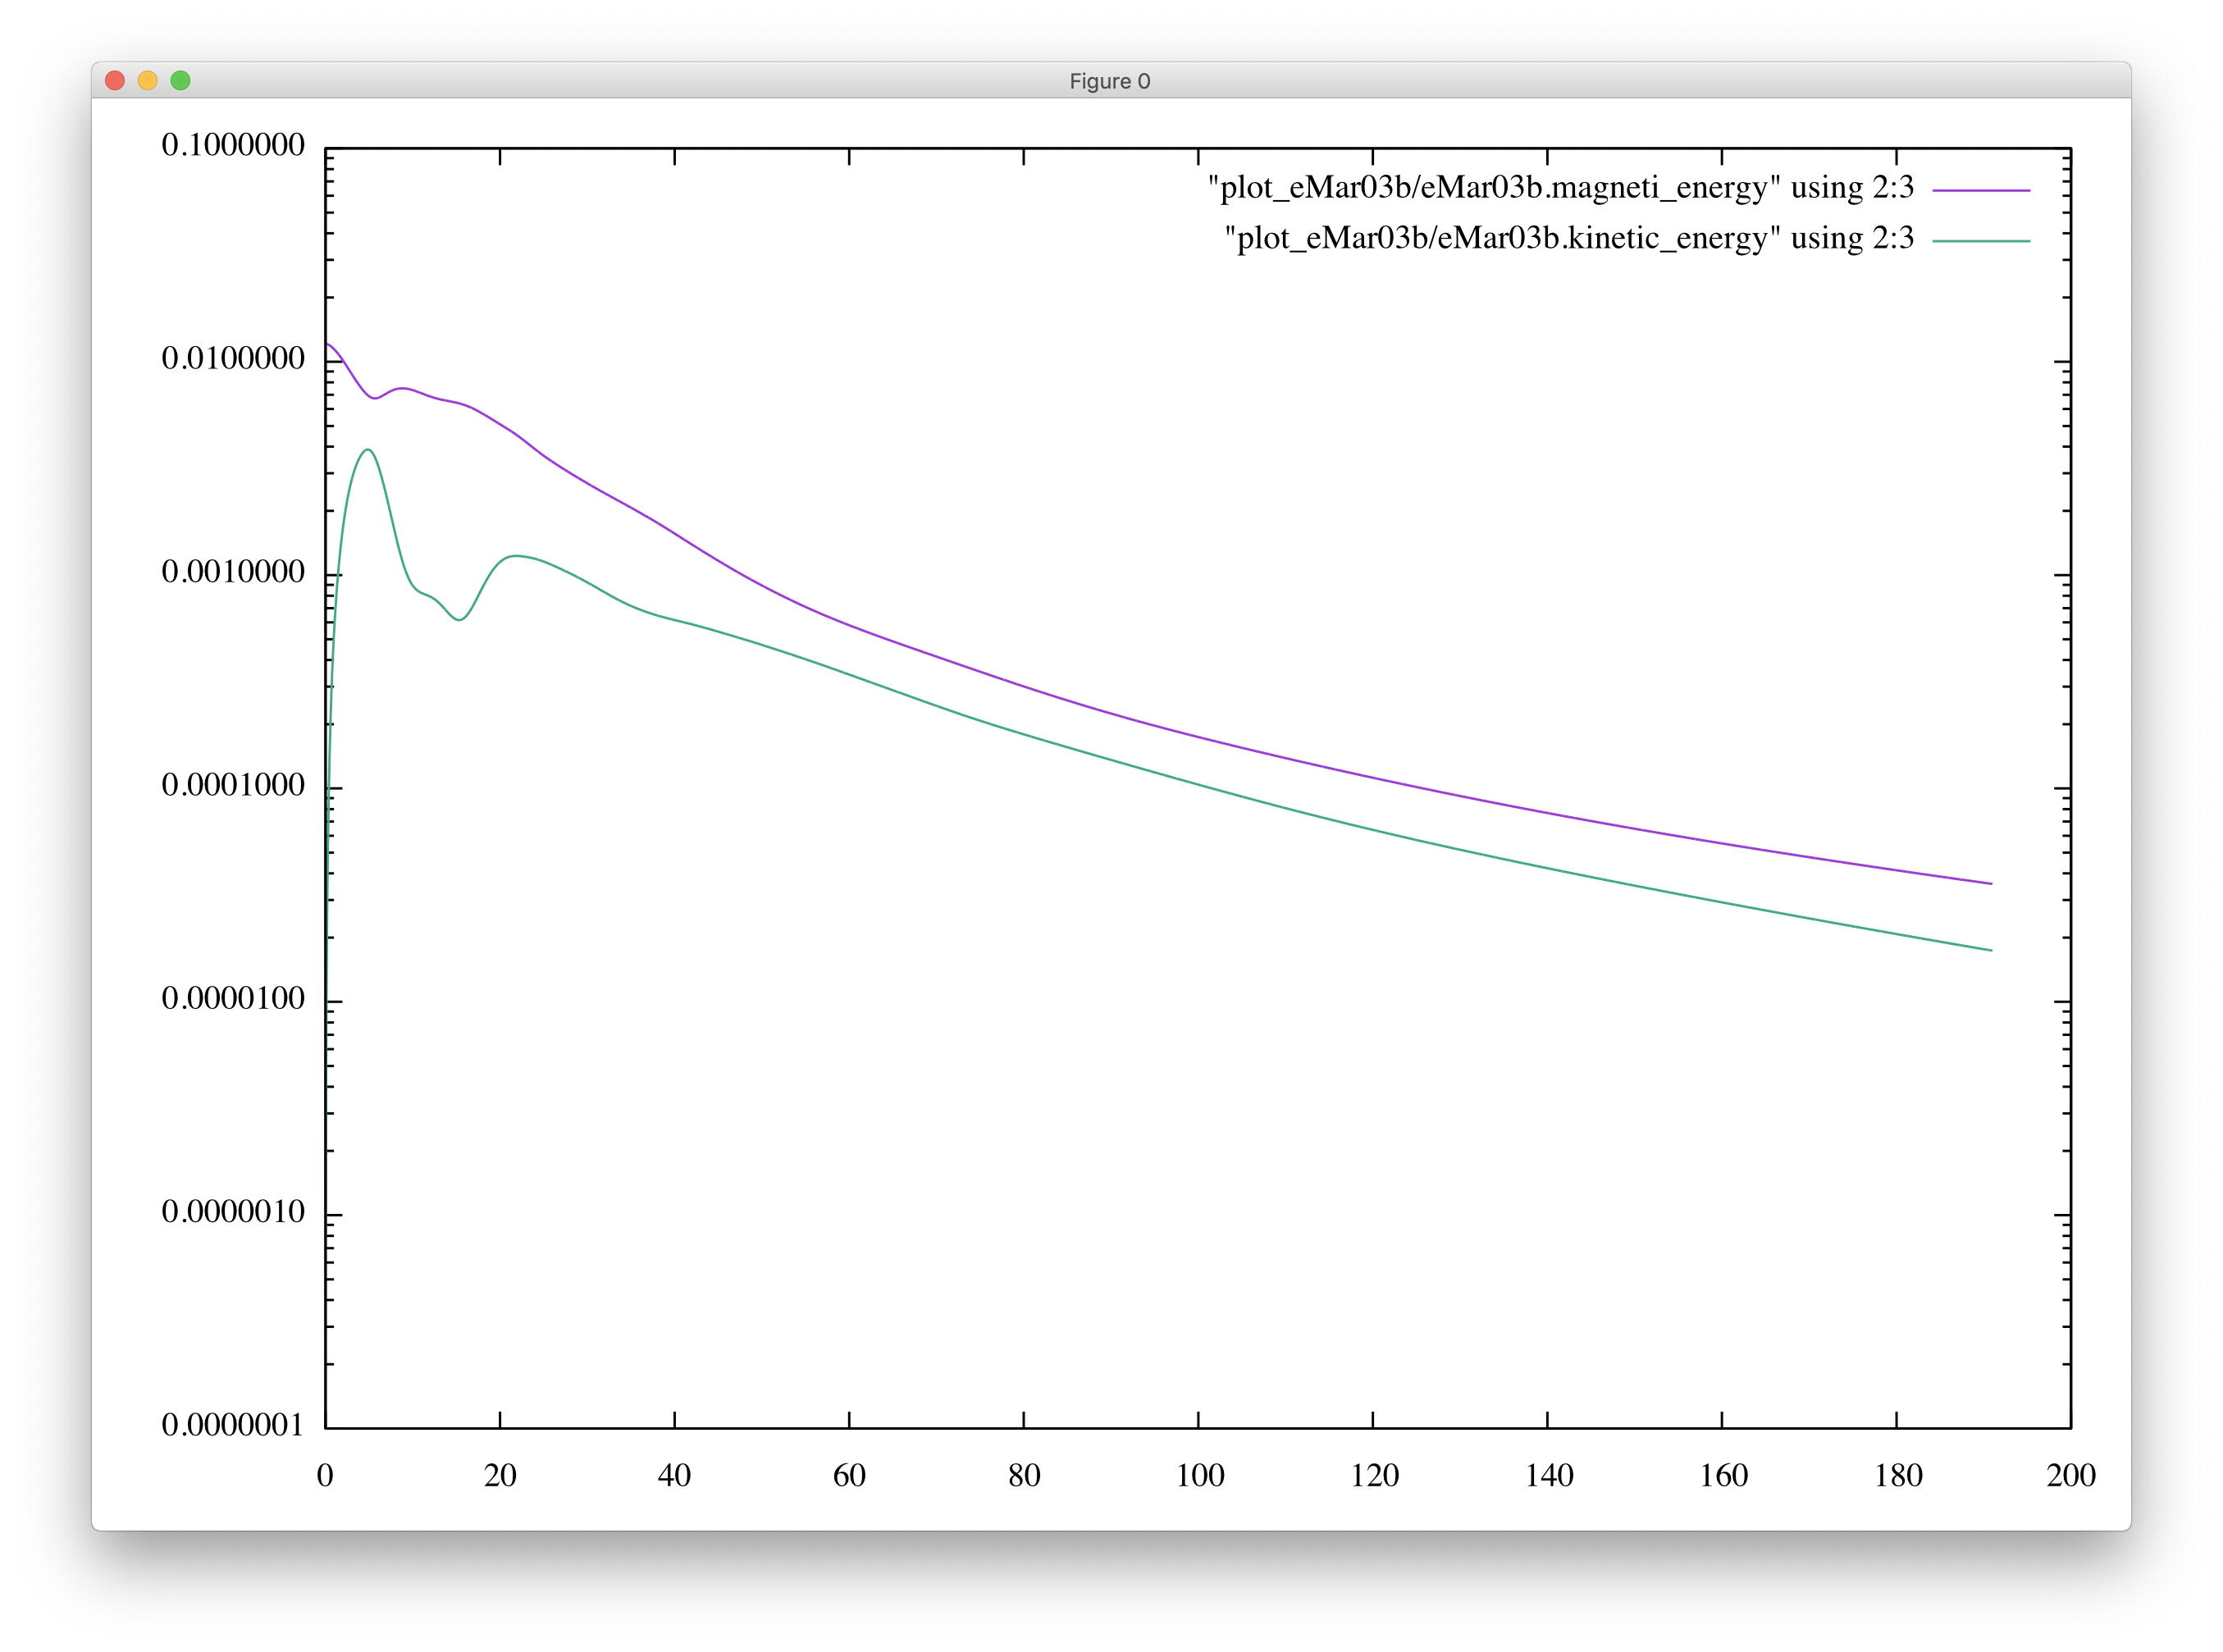
\includegraphics[height=0.5\textheight,width=0.7\hsize,angle=0,keepaspectratio]{./Image/L3M2_graph.png}
%\caption{Relaxation of total magnetic(purple line) and flow(green line) energy in $(l,m)=(3,2)$.} \label{L3M2_graph}
%\end{figure}
%\begin{figure}[H]
%\centering
%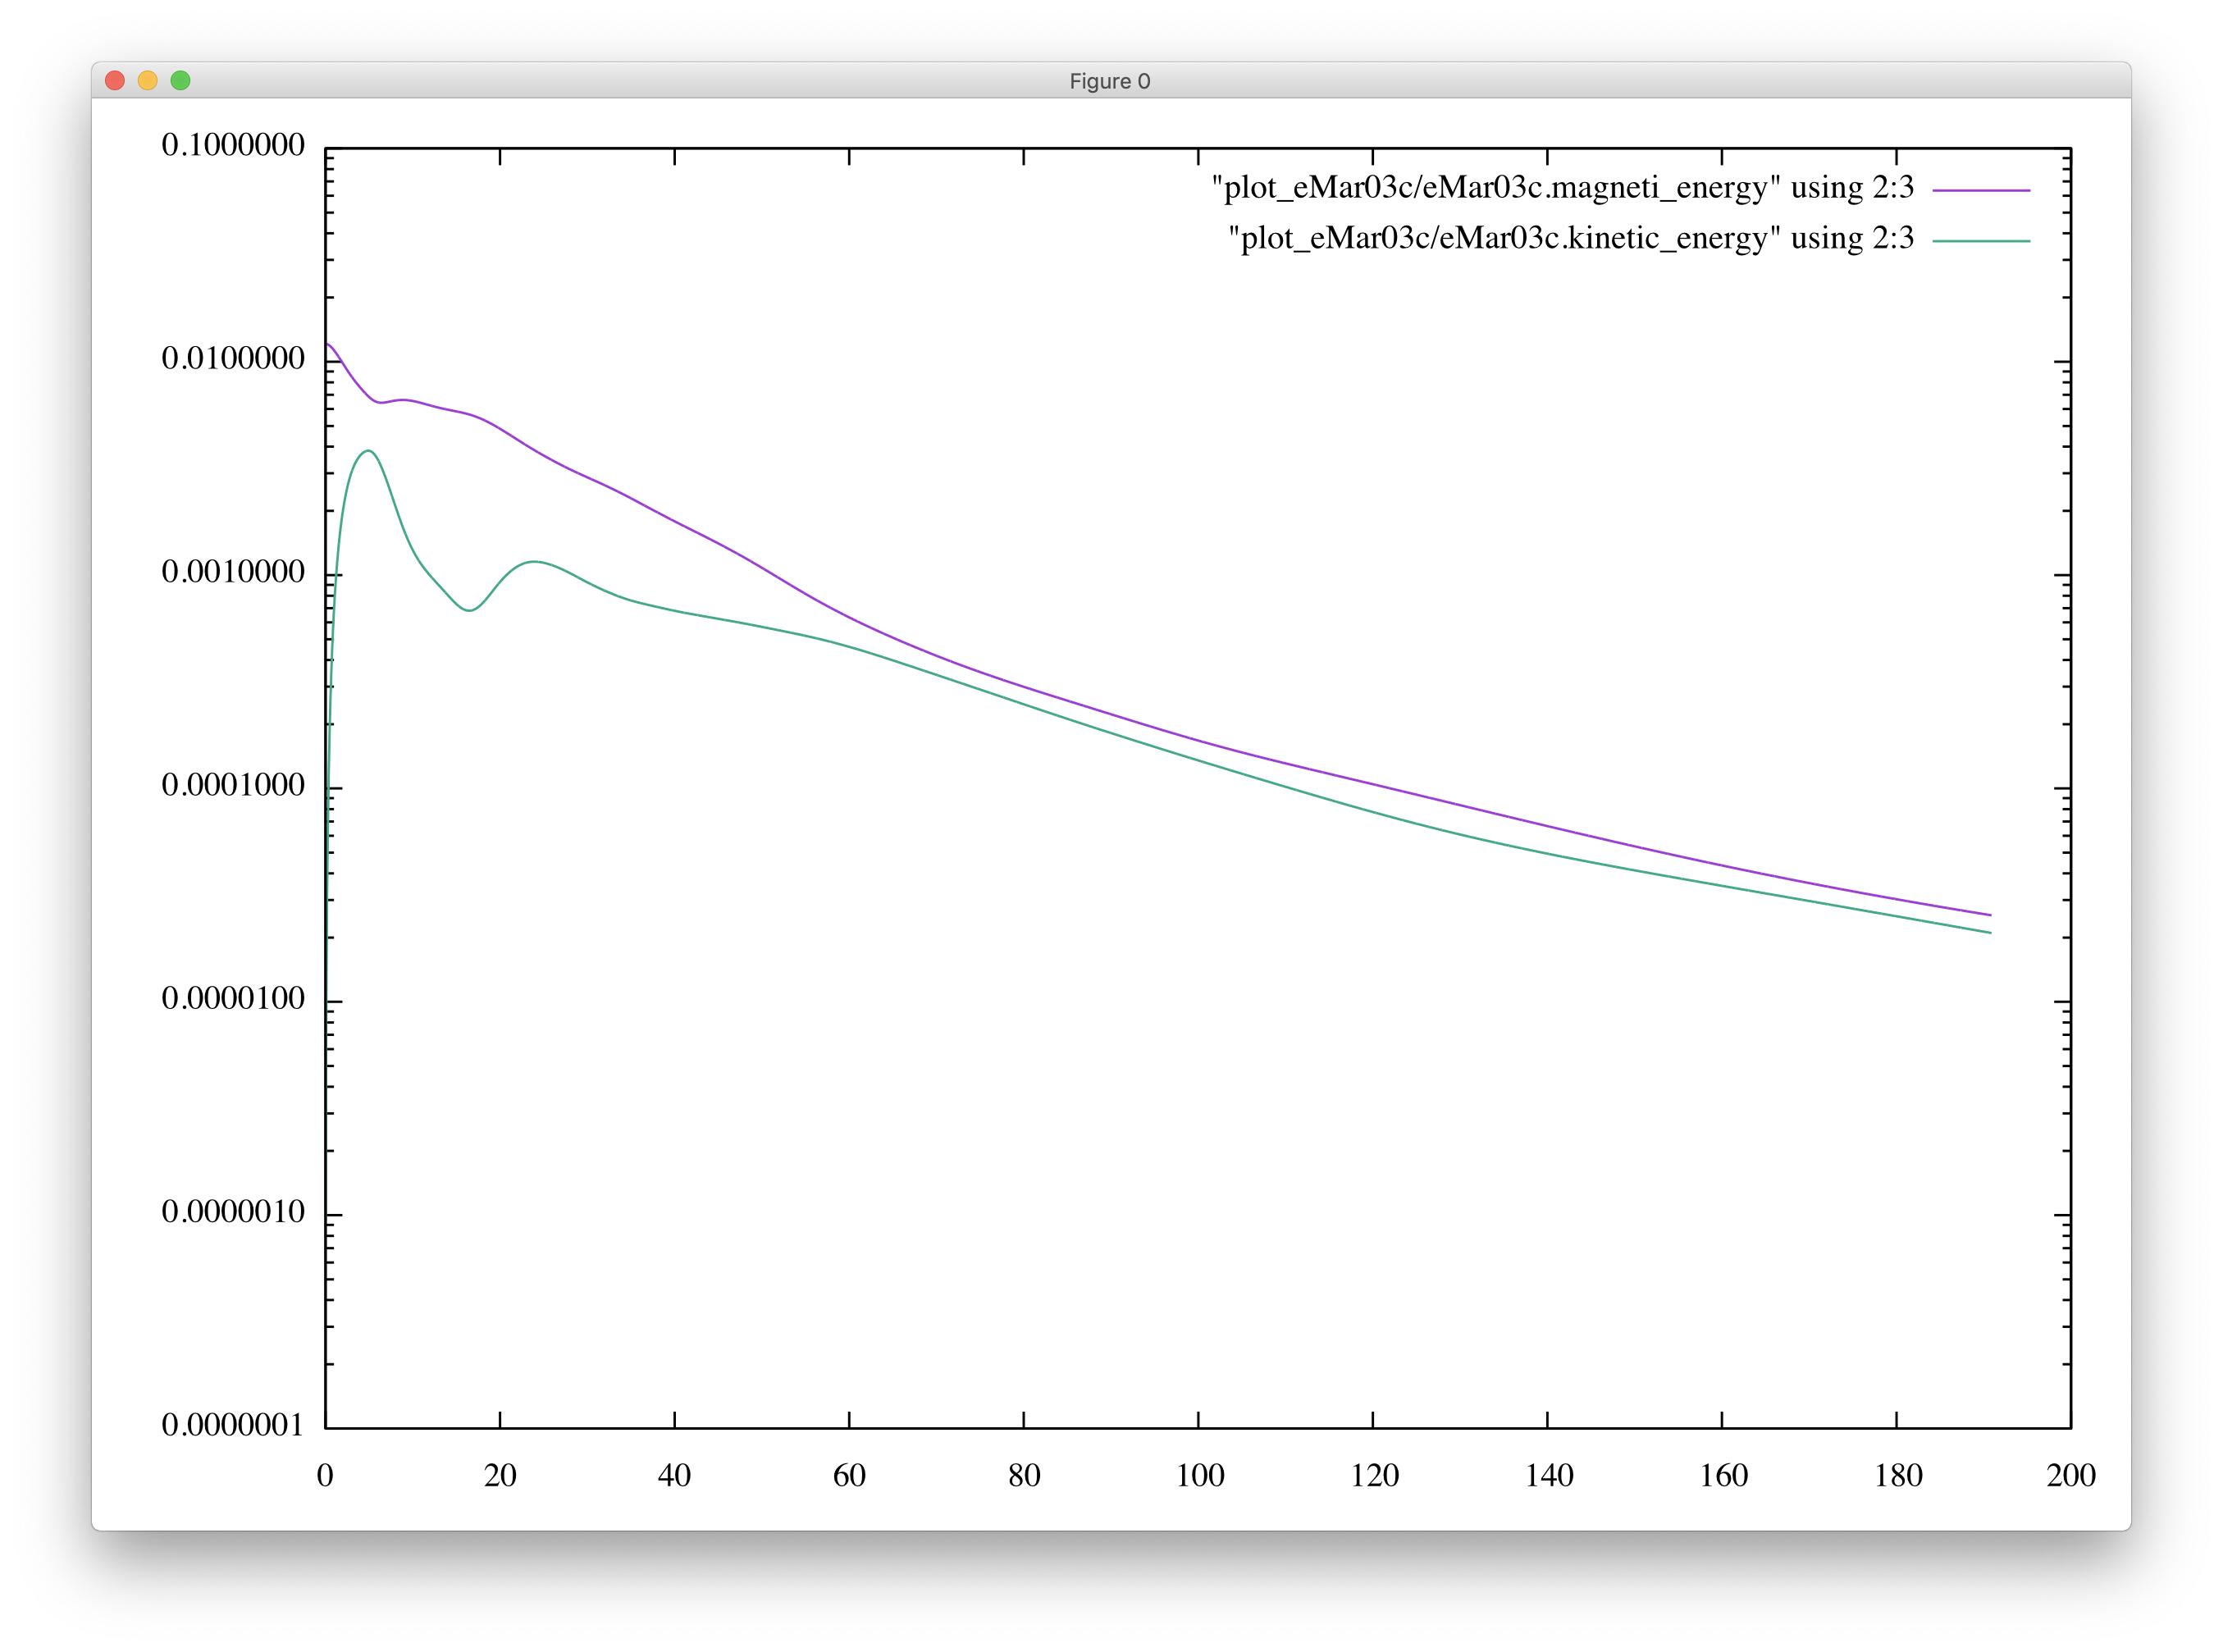
\includegraphics[height=0.5\textheight,width=0.7\hsize,angle=0,keepaspectratio]{./Image/L3M3_graph.png}
%\caption{Relaxation of total magnetic(perple line) and flow(green line) energy in $(l,m)=(3,3)$.} \label{L3M3_graph}
%\end{figure}

\begin{figure}[H]
\centering
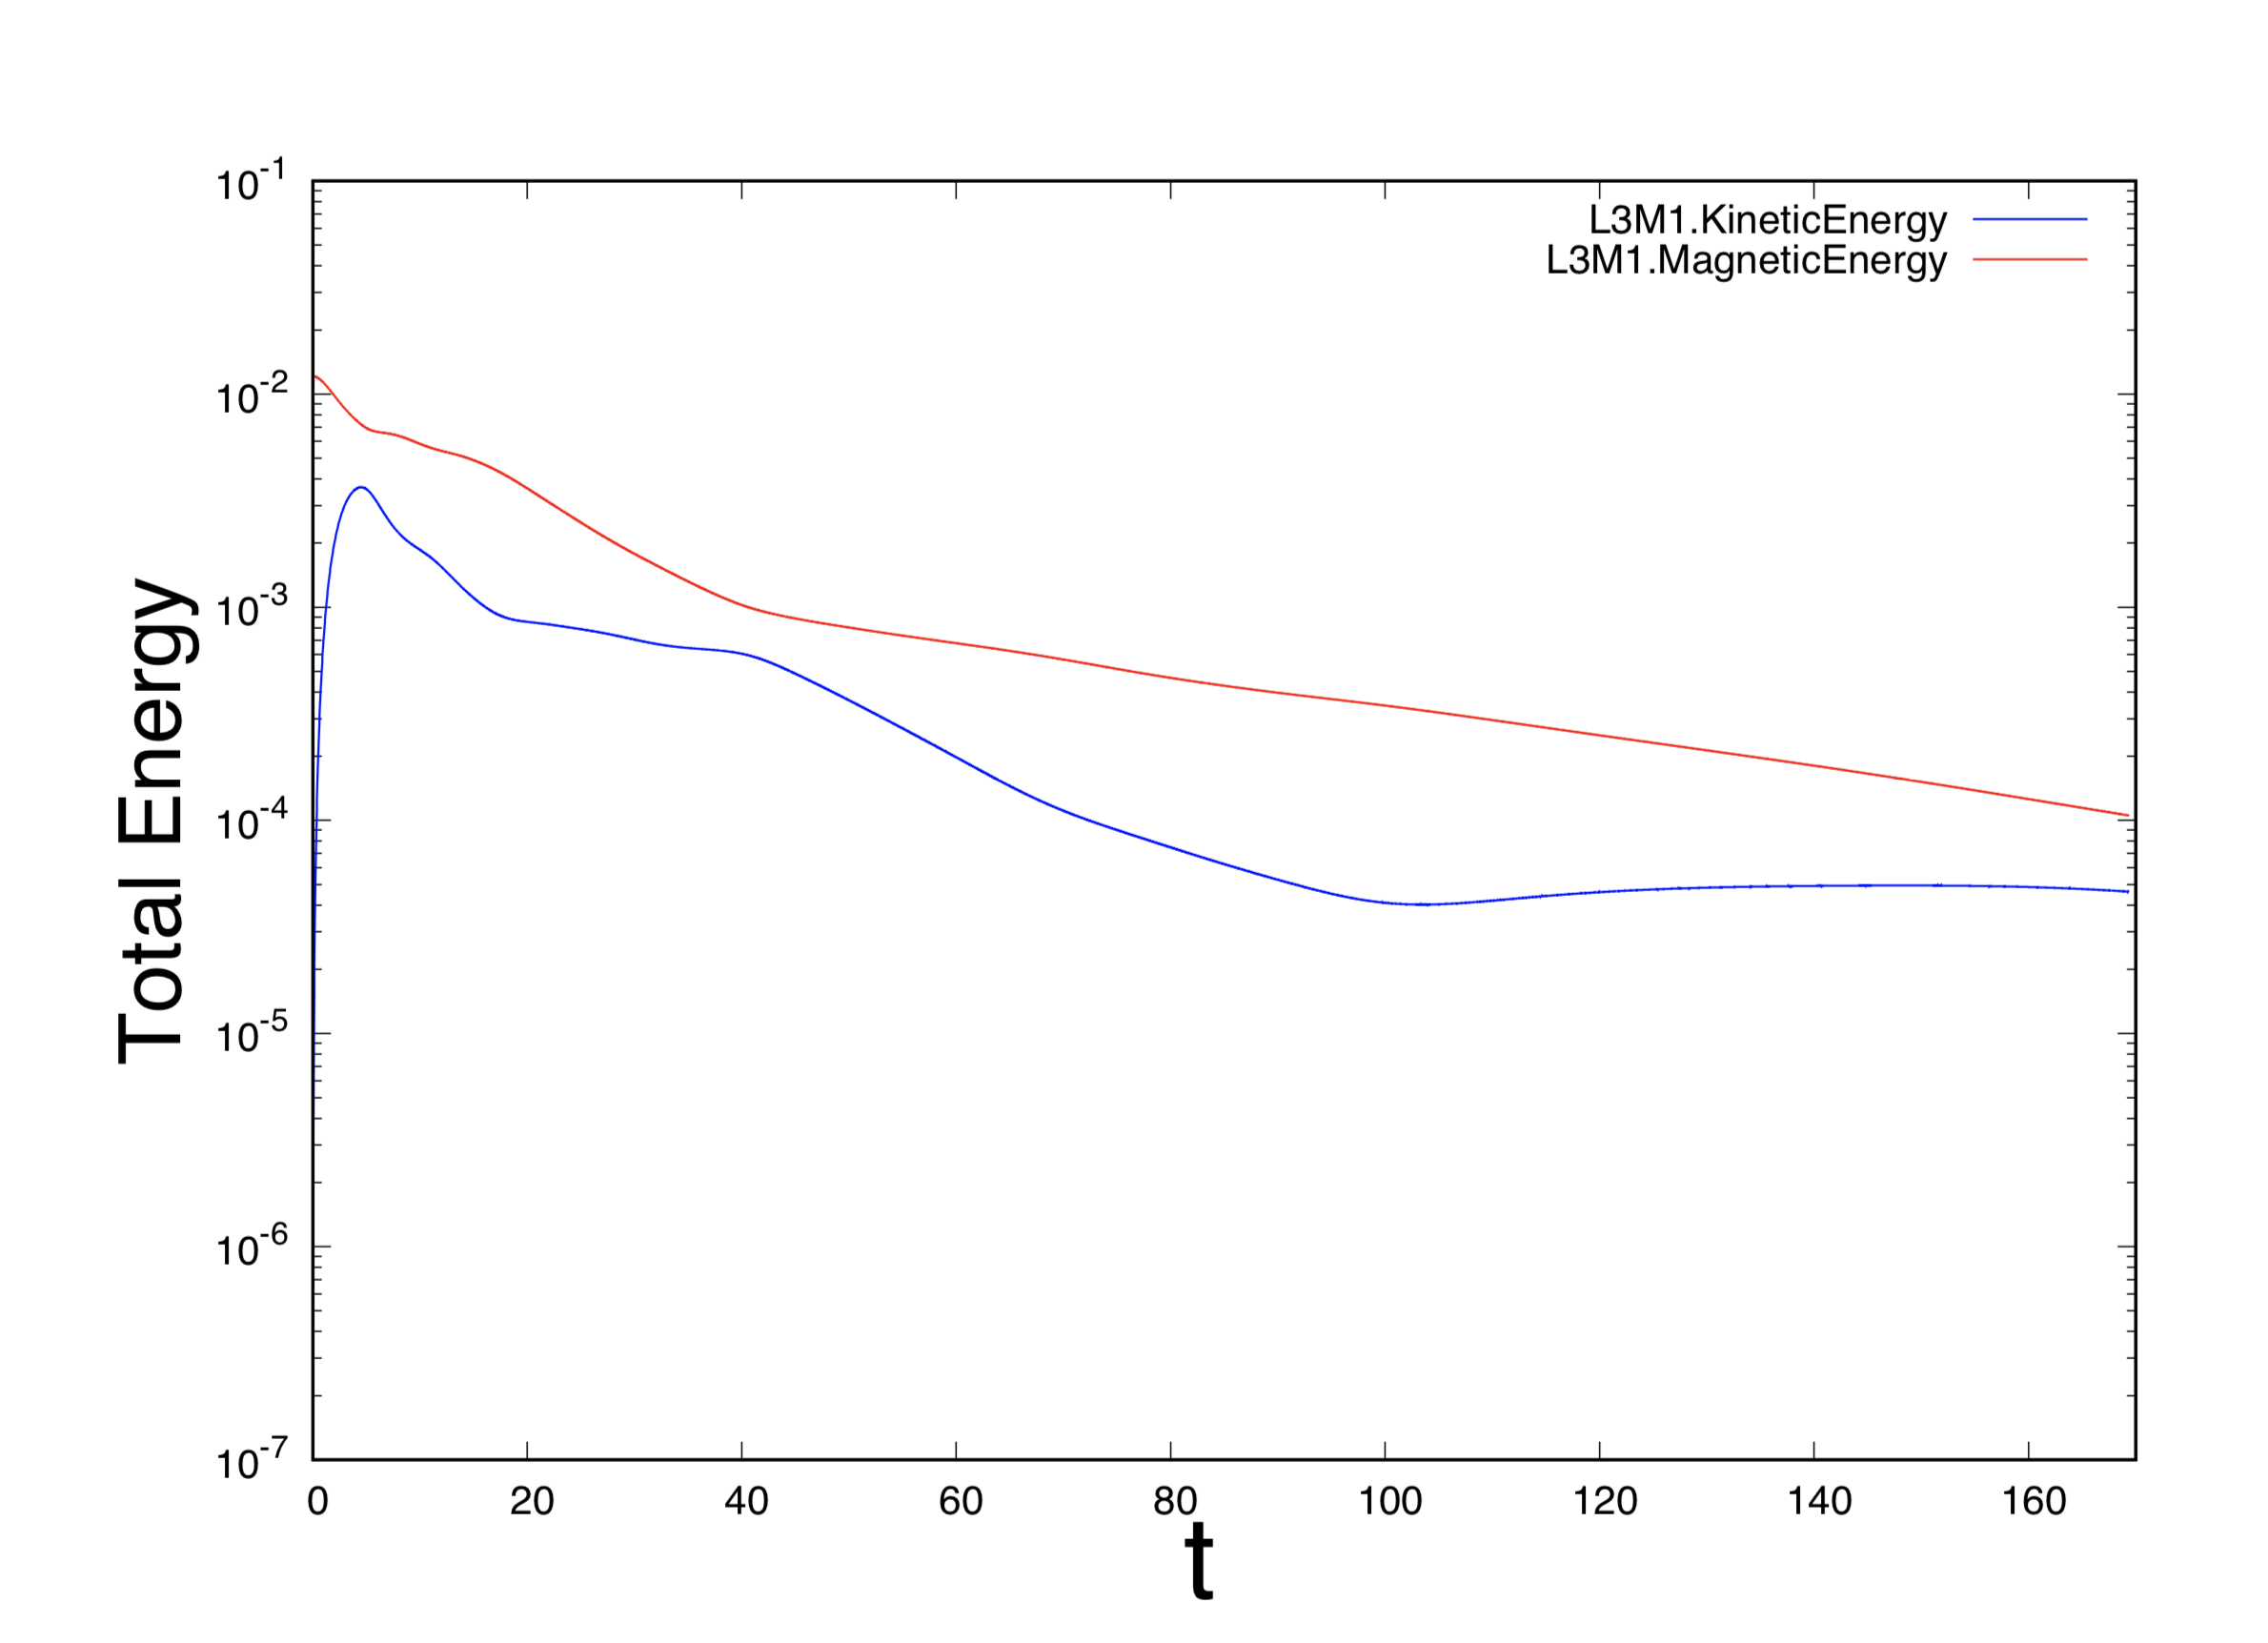
\includegraphics[height=0.5\textheight,width=0.7\hsize,angle=0,keepaspectratio]{./Image/L3M1_graph2.png}
\caption{Relaxation of total magnetic(red line) and flow(blue line) energy in $(l,m)=(3,1)$.} \label{L3M1_graph}
\end{figure}
\begin{figure}[H]
\centering
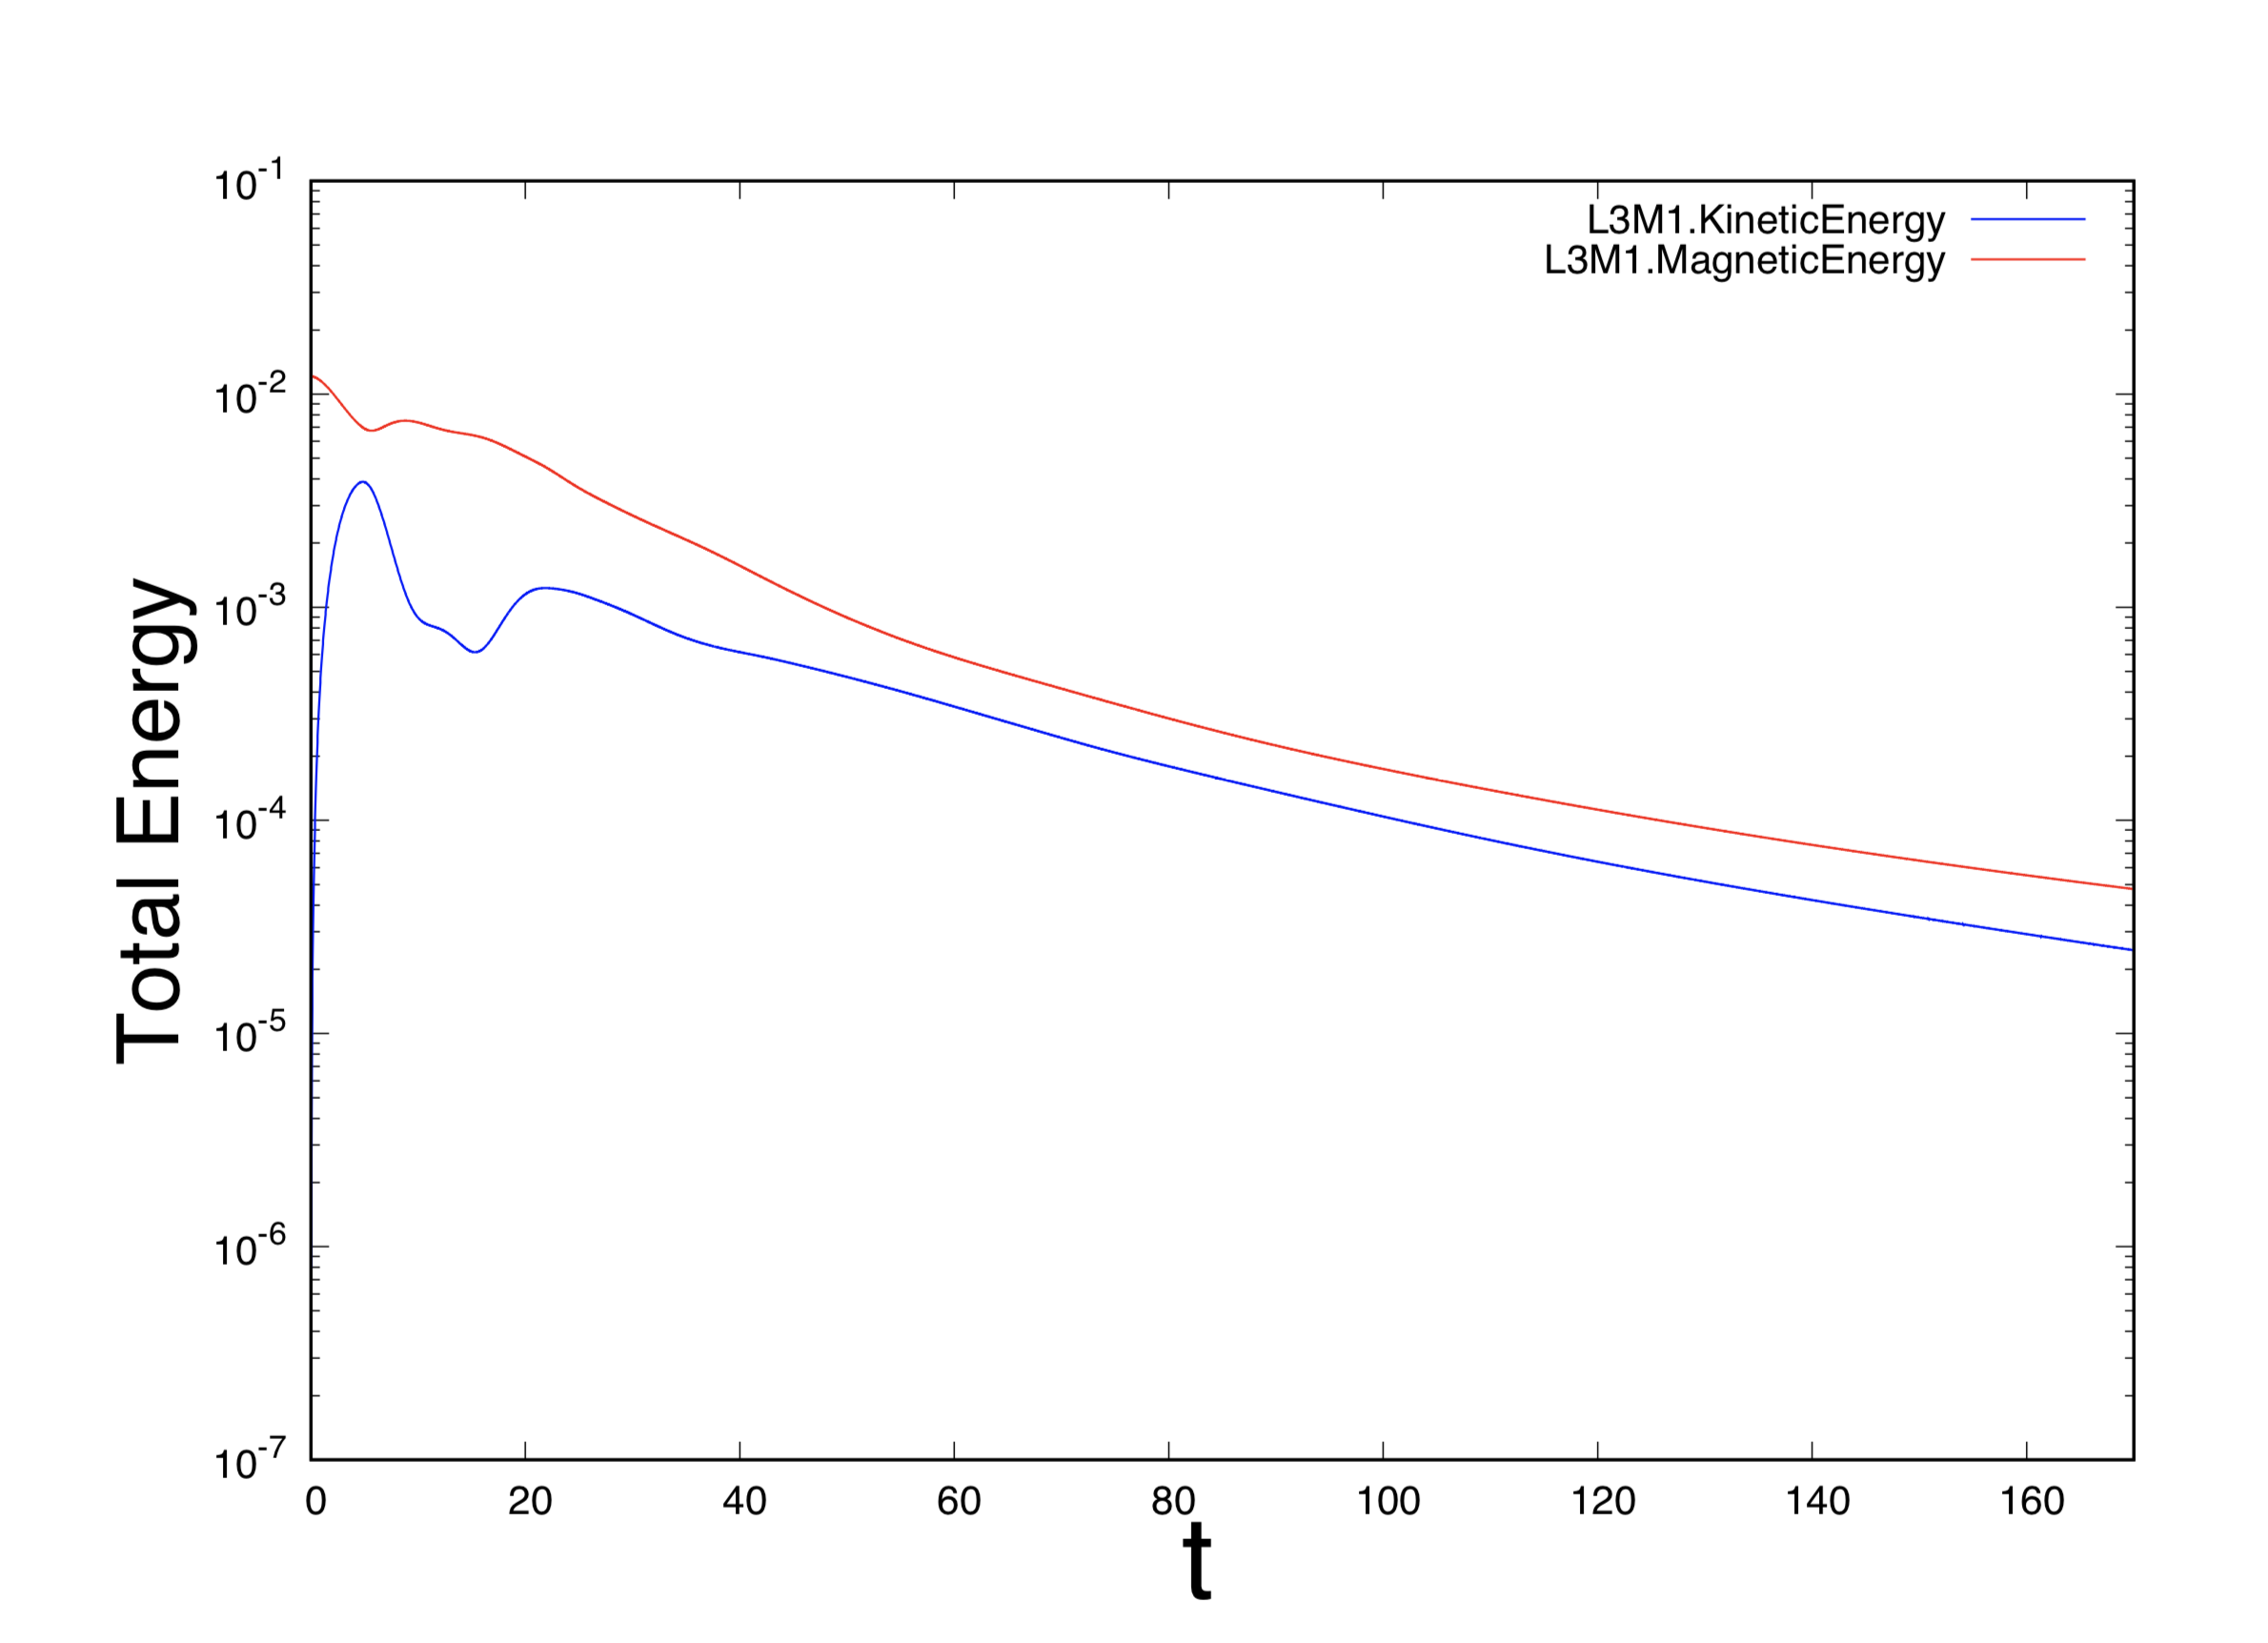
\includegraphics[height=0.5\textheight,width=0.7\hsize,angle=0,keepaspectratio]{./Image/L3M2_graph2.png}
\caption{Relaxation of total magnetic(red line) and flow(blue line) energy in $(l,m)=(3,2)$.} \label{L3M2_graph}
\end{figure}
\begin{figure}[H]
\centering
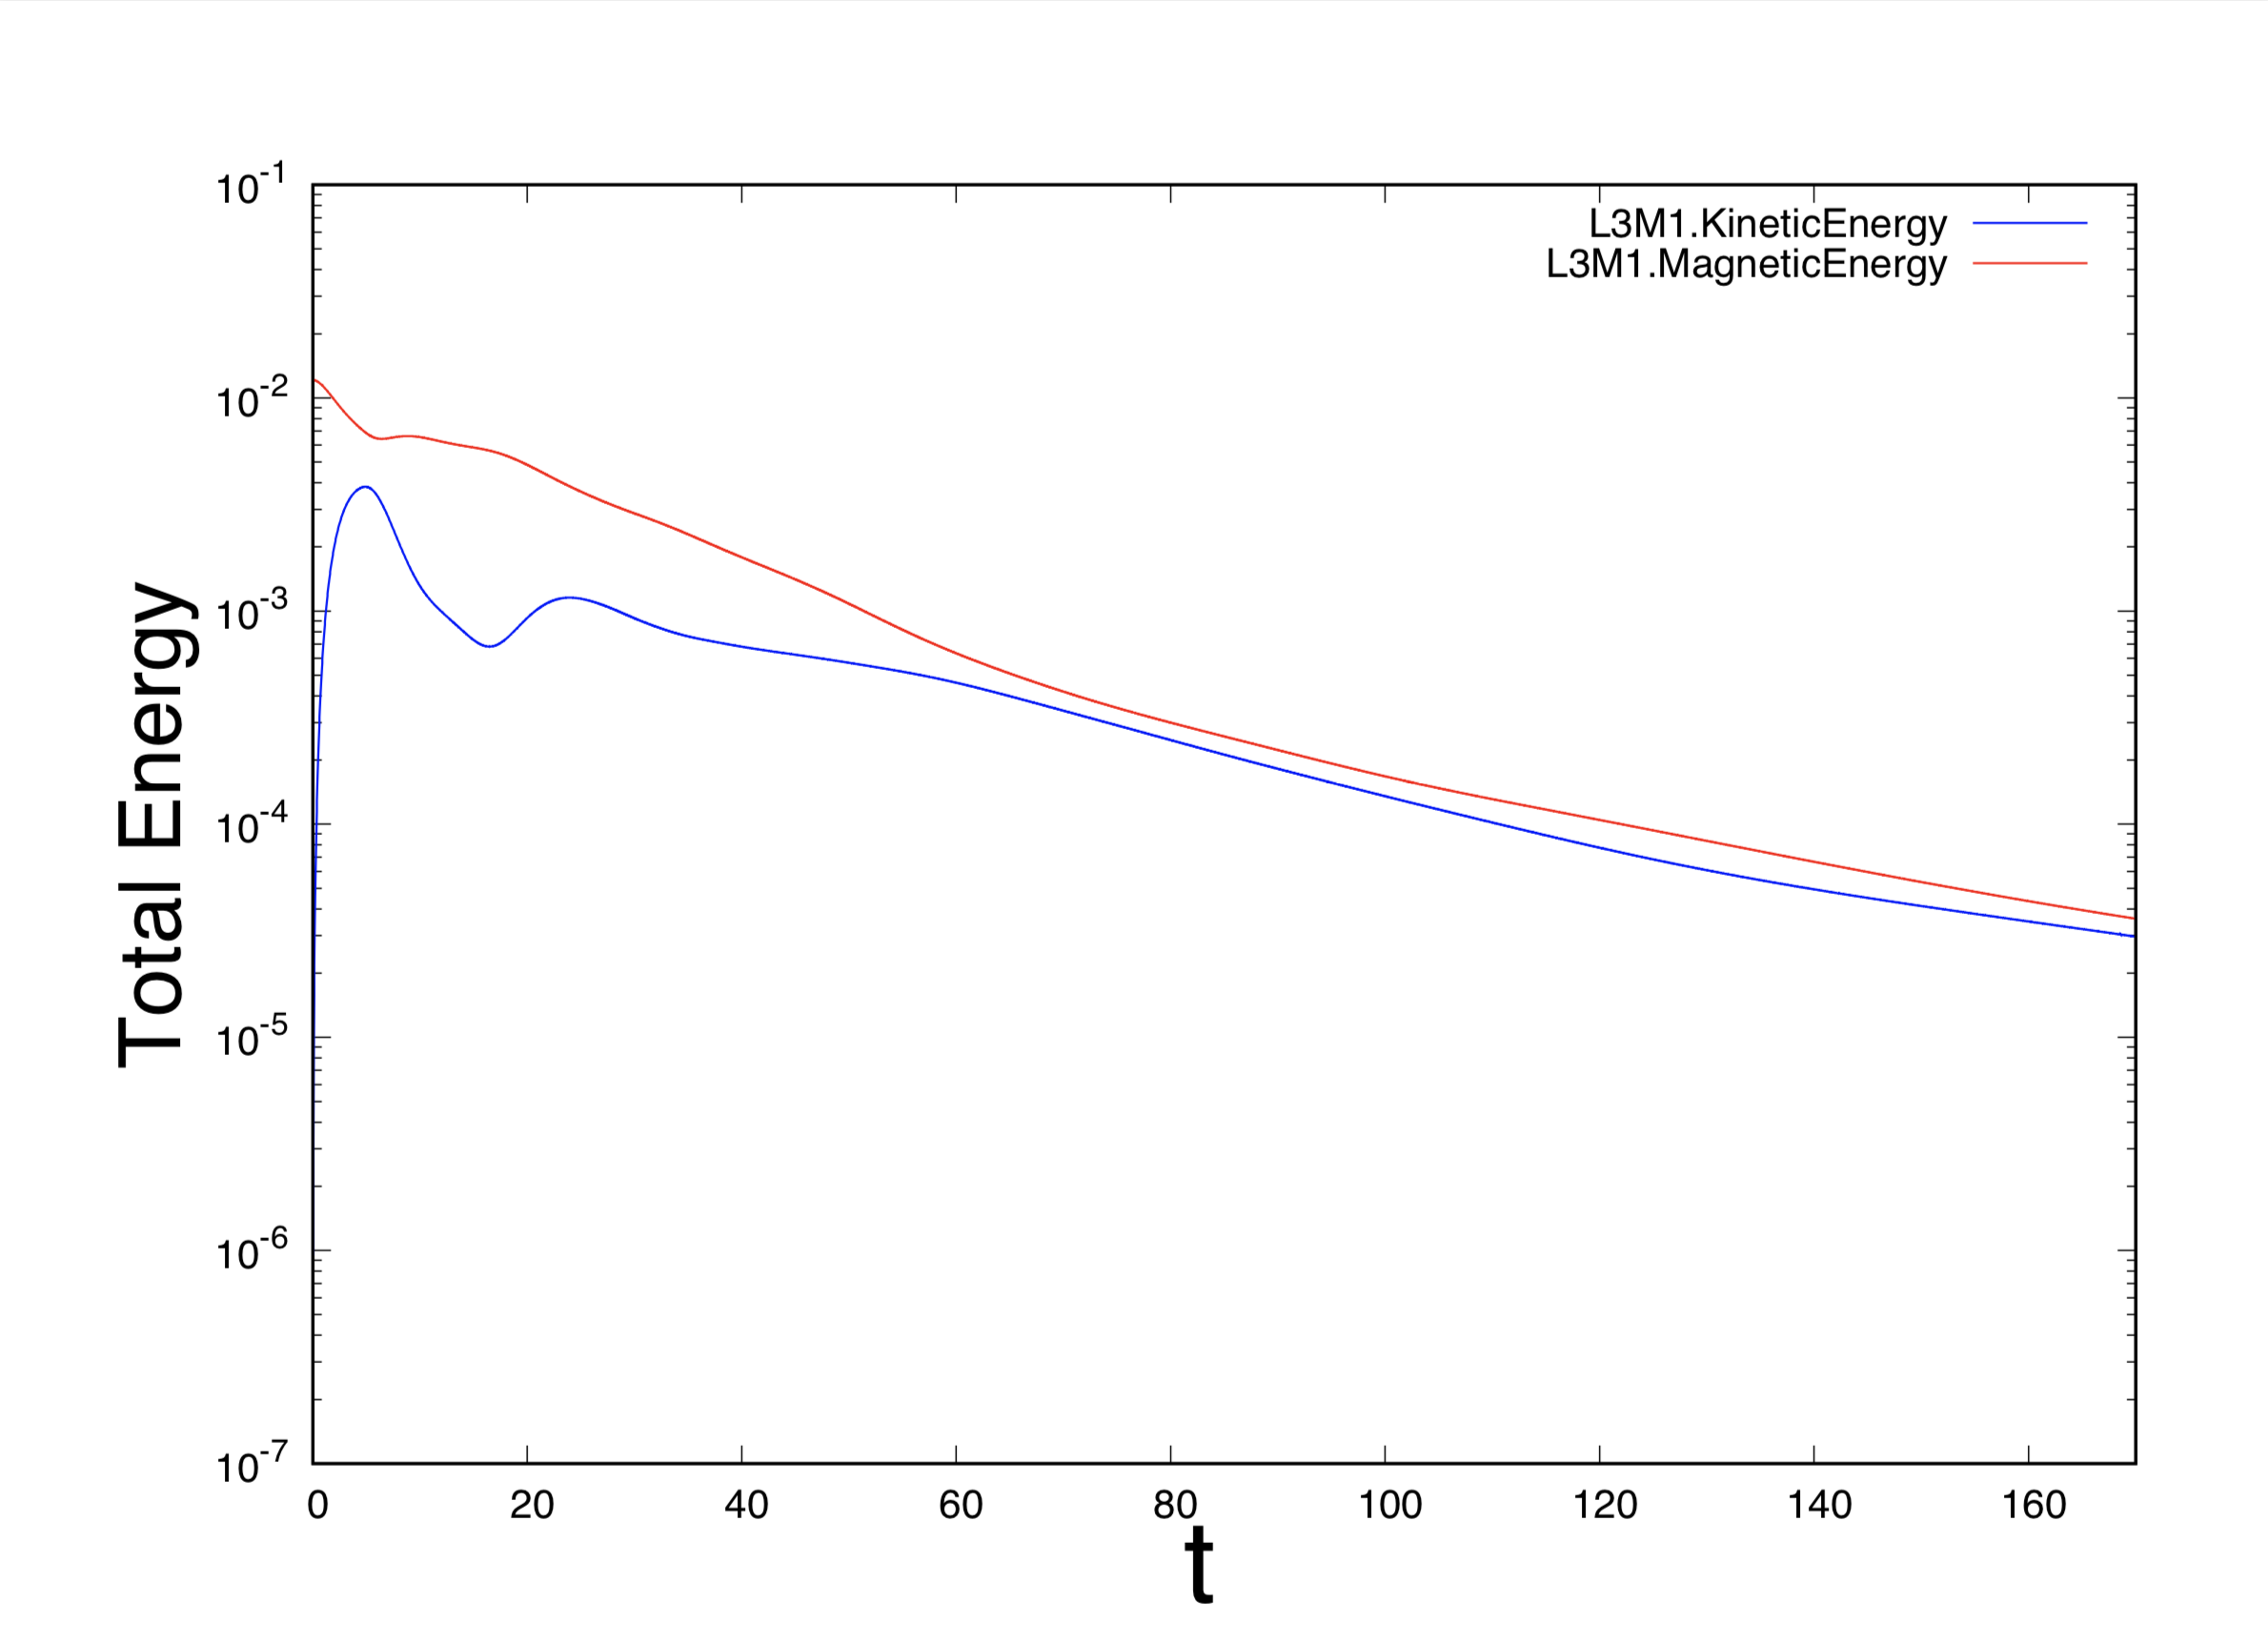
\includegraphics[height=0.5\textheight,width=0.7\hsize,angle=0,keepaspectratio]{./Image/L3M3_graph2.png}
\caption{Relaxation of total magnetic(red line) and flow(blue line) energy in $(l,m)=(3,3)$.} \label{L3M3_graph}
\end{figure}


いずれの場合も磁気エネルギーと運動エネルギーがお互いにエネルギーを交換しあい振動していることがわかる。そして最終的に振動は落ち着き、双方がゆっくりと減衰している。一番興味があるのはゆっくりと減衰しているこの時で、それぞれグラフがプロットしている時刻の最大値付近では系が十分緩和していると考えられる。


\subsection{緩和状態の三次元構造}
以下に緩和状態の磁力線および流線の3次元構造を示す(Fig.\ref{L3M1_relaxed}-\ref{L3M3_relaxed})。流線は流れのベクトル図に重ね合わせている。

\begin{figure}[H]
\centering
\includegraphics[height=0.5\textheight,width=1.0\hsize,angle=0,keepaspectratio]{./Image/relaxedL3M1.png}
\caption{Stream tracer of relaxed magnetic field(left), and flow(right) in $(l,m)=(3,1)$.} \label{L3M1_relaxed}
\end{figure}
\begin{figure}[H]
\centering
\includegraphics[height=0.5\textheight,width=1.0\hsize,angle=0,keepaspectratio]{./Image/relaxedL3M2.png}
\caption{Stream tracer of relaxed magnetic field(left), and flow(right) in $(l,m)=(3,2)$.} \label{L3M2_relaxed}
\end{figure}
\begin{figure}[H]
\centering
\includegraphics[height=0.5\textheight,width=1.0\hsize,angle=0,keepaspectratio]{./Image/relaxedL3M3.png}
\caption{Stream tracer of relaxed magnetic field(left), and flow(right) in $(l,m)=(3,3)$.}\label{L3M3_relaxed}
\end{figure}

これらのうち流れ場の構造の特徴が特に顕著だと思われる$(l,m)=(3,3)$を重点的に解析する。

\subsection{$(l,m)=(3,3)$の緩和状態}
以下に$(l,m)=(3,3)$の緩和時の速度場半径成分$v_r$(Fig.\ref{vr_L3M3})、および磁場経度成分$b_\phi$(Fig.\ref{bp_L3M3})それぞれの球面分布とその球面で球面調和関数展開したときの係数${|c|}^2$のグラフを示す。半径$r=0.9$とし、球面分布の可視化手法にモルワイデ図法を用いた。

\begin{figure}[H]
\centering
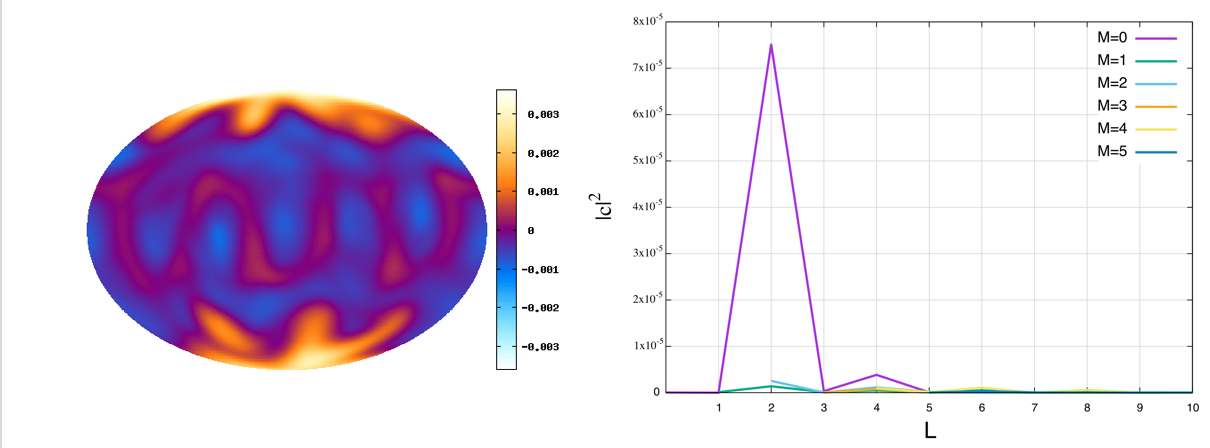
\includegraphics[height=0.5\textheight,width=1.0\hsize,angle=0,keepaspectratio]{./Image/vr_L3M3.png}
\caption{Snapshots in logitude-latitude Mollwide Projection of relaxed longitude magnetic field $v_r$ (left) and coefficients of spherical harmonics for surface of sphere $r=0.9$ (right) in $(l,m)=(3,3)$.}\label{vr_L3M3}
\end{figure}

\begin{figure}[H]
\centering
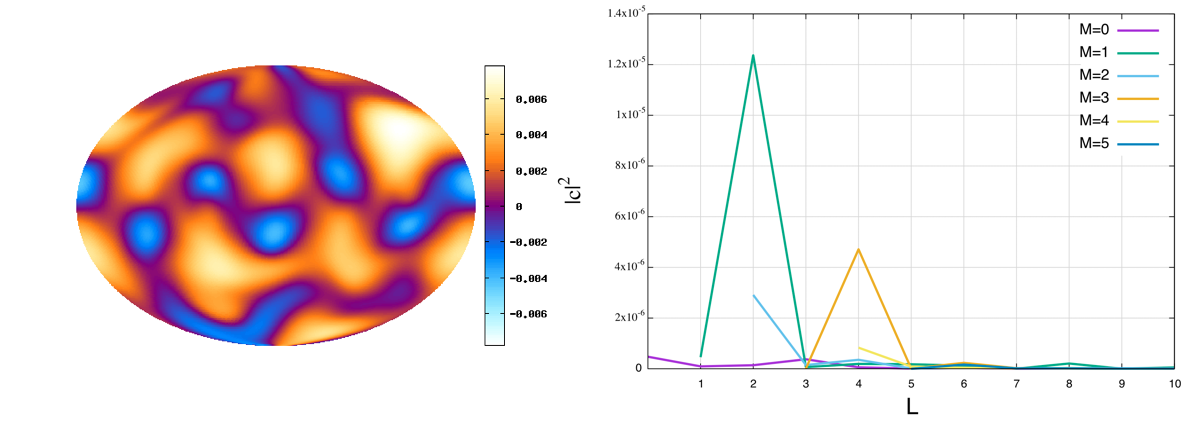
\includegraphics[height=0.5\textheight,width=1.0\hsize,angle=0,keepaspectratio]{./Image/bp_L3M3.png}
\caption{Snapshots in logitude-latitude Mollwide Projection of relaxed longitude magnetic field $b_\phi$ (left) and coefficients of spherical harmonics for surface of sphere $r=0.9$ (right) in $(l,m)=(3,3)$.}\label{bp_L3M3}
\end{figure}
%\begin{figure}[H]
%\centering
%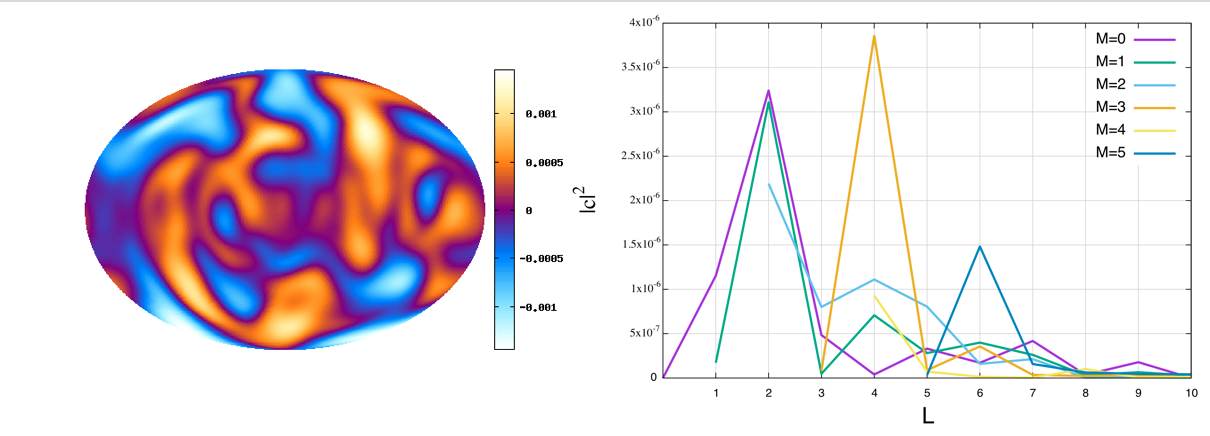
\includegraphics[height=0.5\textheight,width=1.0\hsize,angle=0,keepaspectratio]{./Image/br_L3M3.png}
%\caption{Equatonal plane(top), and meridian plane(bottom) of stream tracer: relaxed magnetic field(left) and flow(right) in $(l,m)=(3,3)$.}\label{br_L3M3}
%\end{figure}

Fig.\ref{vr_L3M3}より、緩和状態において表面付近の$v_r$の$Y_2^0$成分が強く、流れ場は四重極状に緩和していることがわかる。これは球の中心方向へ縮む初期磁力線に流体が凍りつき、両極から流れ出し、赤道付近でまた中心へ潜り込むという流れのサイクルが生まれたことを示唆している。

また初期の$b_\phi$(Fig.\ref{b0p_L3M3})と緩和前の$b_\phi$(Fig.\ref{bp_L3M3})を比べてみると、初期の$b_\phi$は$Y_4^3$成分が卓越していたのに対し、緩和後では$Y_2^1$成分が強くなっている。これは$Y_4^3$よりも$Y_2^1$のほうが構造的に安定しているからであり、系が自発的に緩和した結果である。

以下にFig.\ref{L3M3_relaxed}の赤道断面(Fig.\ref{clip_L3M3_xy}上)と子午断面(Fig.\ref{clip_L3M3_xy}下)を示す。
\begin{figure}[H]
\centering
\includegraphics[height=0.5\textheight,width=0.7\hsize,angle=0,keepaspectratio]{./Image/clip_L3M3_xy.png}
\includegraphics[height=0.5\textheight,width=0.7\hsize,angle=0,keepaspectratio]{./Image/clip_L3M3_xz.png}
\caption{Equatonal plane(top), and meridian plane(bottom) of stream tracer: relaxed magnetic field(left) and flow(right) in $(l,m)=(3,3)$.}\label{clip_L3M3_xy}
\end{figure}
この図より、上記に述べたように流体が6つの磁力線のリングの中心を通り、両極へ流れるというサイクルができていることがわかる。また磁力線は赤道付近で初期の6つの輪の構造を維持しつつ、中心から両極にかけては流れによって引き延ばされている。

以上より緩和状態の構造は以下のような模式図(Fig.\ref{L3M3_cartoon})で表される。赤色は磁力線、青色は流れ場を表している。

\begin{figure}[H]
\centering
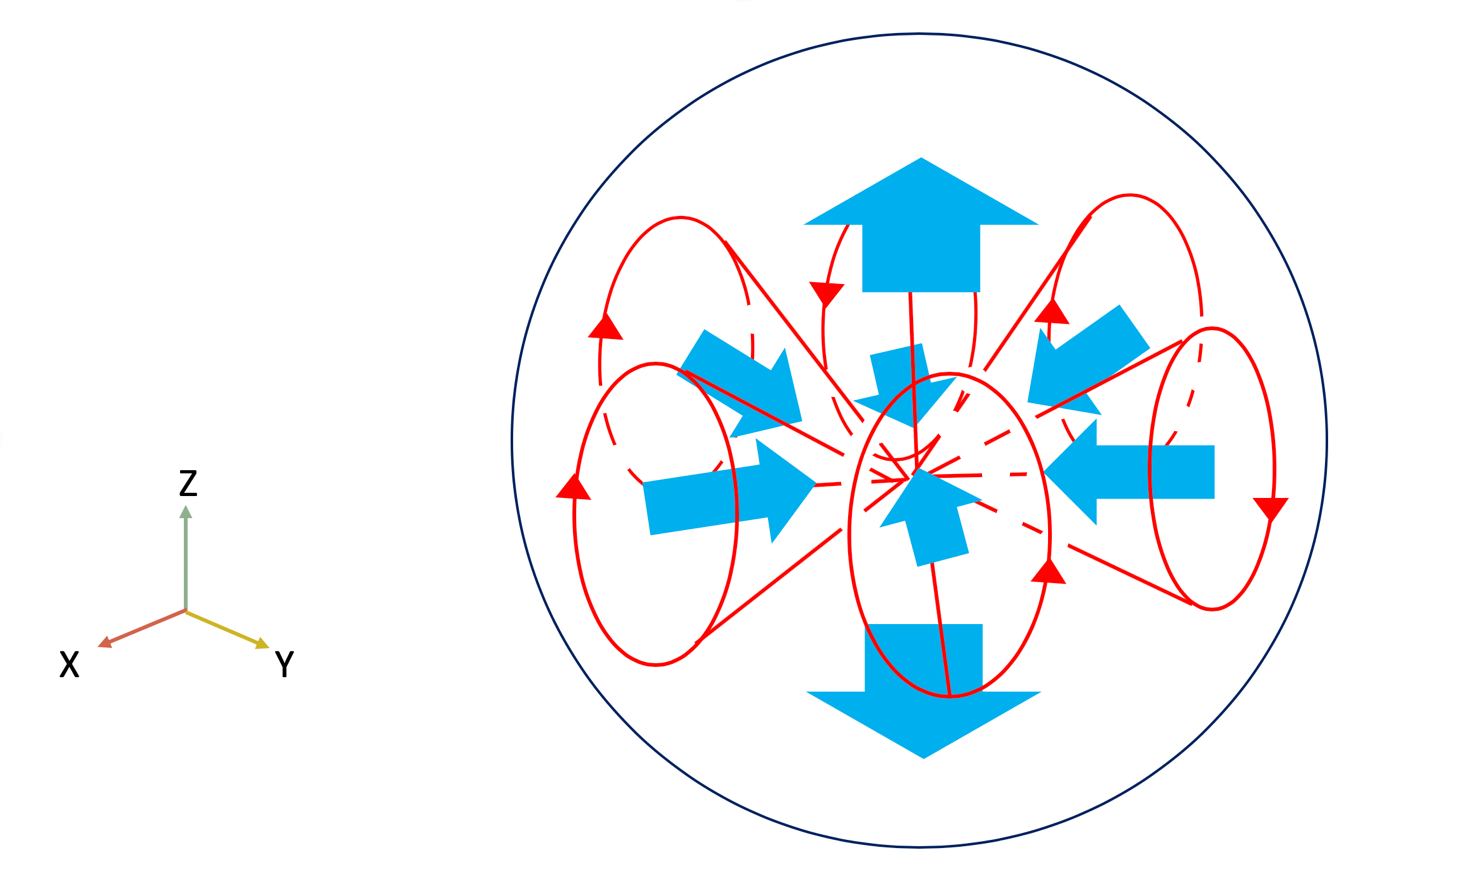
\includegraphics[height=0.5\textheight,width=1.0\hsize,angle=0,keepaspectratio]{./Image/relaxedL3M3_cartoon2.png}
\caption{3D structure of relaxed magnetic field(red), and flow(blue) in $(l,m)=(3,3)$.}\label{L3M3_cartoon}
\end{figure}

まとめると速度場の遷移は以下のようになる。
\begin{enumerate}
 % \renewcommand{\labelenumi}{(\arabic{enumi})}
\item 磁力線のリングから中心に向かう流れが起きる。
\item 球の中心付近で流れが衝突する。
\item 衝突した流れは両極方向へ向きが変わる。
\item 極にたどり着いた流れは境界に当たることで、また磁力線のリングの中心へ向かう(1に戻る)。
\end{enumerate}
また磁場の遷移は以下のようになる。
\begin{enumerate}
\item 球表面付近の磁力線のリングが縮まり流れの駆動力になる。
\item 縮んだ磁力線のリングは流れに運ばれ中心付近に集まる。
\item 集まった磁力線のリングは流れ場によって両極に引き伸ばされる。
\item 引き伸ばされた磁力線のリングは球の表面付近を通り、元の磁力線のリングの中心へ向かう(1に戻る)。
\end{enumerate}


%=============================================
\section{結論}
エネルギーが不安定な状態から安定な状態に落ち着くという緩和は自然界の多くに見られ、MHD流体も例外ではない。MHD流体の緩和状態は領域内で力が全く働かないforce-free状態であるというTaylor理論は多くの実験に適用されてきた。しかし、Taylor理論は運動エネルギーが無視され、緩和状態では流れが存在しないと仮定されている。そこで本研究では球ジオメトリ内部でのMHD流体の緩和についてスーパーコンピュータを用いた計算機シミュレーションで調べた。

本研究の設定として、完全導体かつ外部から力が働かない断熱の境界である球にMHD流体が入っている状況を想定した。また初期条件として球面調和関数を磁場を与えた。球面調和関数で表されるリング上の磁場は、磁場の輪が縮む方向にローレンツ力が働きそれが起動力となってMHD流体が動き出した。

計算機でシミュレートするにあたって球座標格子を用いた場合、格子点の集中が避けられないため計算にコストがかかってしまう。そこで本研究では重合格子であるYin--Yang--Zhong格子を用いることでコストがかからない計算を行うことができた。

本研究では弱い磁場を想定していたので、これからは強い磁場についても考察していく必要がある。


%=============================================
\section*{謝辞}
\addcontentsline{toc}{section}{謝辞}
本研究を進めるにあたって、熱心に指導していただいた陰山聡教授に深く感謝いたします。
%=============================================
\newpage
% 参考文献
%=============================================
%\section*{参考文献}
\addcontentsline{toc}{section}{参考文献}
\bibliographystyle{junsrt}
\bibliography{bibtex.bib}
\end{document}